\documentclass[12pt]{article}

\usepackage{fullpage}
\usepackage{graphicx}
\usepackage{graphics}
\usepackage{mdwlist}
\usepackage{float}

% christos: these look closer to NSF specs\dots
\setlength{\oddsidemargin}{0.0in}
\setlength{\evensidemargin}{0.0in}
\setlength{\textwidth}{6.5in}
\setlength{\headheight}{0.0in}
\setlength{\topmargin}{0.0in}
% \setlength{\textheight}{9.0in}
\setlength{\textheight}{9in}
\addtolength{\textheight}{-\topmargin}
\addtolength{\textheight}{-\headheight}
\addtolength{\textheight}{-\headsep}
\addtolength{\textheight}{-\footskip}



\begin{document}

\newcommand{\beq}{\begin{equation}}
\newcommand{\eeq}{\end{equation}}
\newcommand{\bit}{\begin{itemize*}}
\newcommand{\eit}{\end{itemize*}}
\newcommand{\goal}[1]{ {\noindent {$\Rightarrow$} \em {#1} } }
\newcommand{\hide}[1]{}
\newcommand{\comment}[1]{ {\footnotesize {#1} } }
\newtheorem{lemma}{Lemma}
\newtheorem{theorem}{Theorem}
\newtheorem{proof}{Proof}
\newtheorem{defn}{Definition}
\newtheorem{algo}{Algorithm}
\newtheorem{observation}{Observation}

\title{15-826 Project Report}


\author{ {\em Chengliang Lian} \\
	    Language Technologies Institute \\
	    CMU\\
	    {\tt clian@andrew.cmu.edu}
	 \and
	 {\em Rui Shen} \\
	     Language Technologies Institute \\
	     CMU\\
	     {\tt ruis@andrew.cmu.edu}
	     }


\maketitle

\section{Survey}
    \label{sec:survey}
    \subsection{Papers read by Chengliang Lian}
The first paper was the GBASE paper by U Kang et al.
\cite{Kang:2012:GEA:2387332.2387347}
\begin{itemize*}
\item {\em Main idea}: 
This paper proposed a efficient way to store, index and query graphs. The basic reasons to focus on this problem is because the precious value of conducting research on graphs like networks and the growing size of graph. The paper address graph mining in three aspects:  graph storage, graph search algorithm and query optimization. There are several features in this system which is very helpful. First, the system runs on distributed system based on hadoop model, which could be scaled out and in to fit in variant throughput and could support parallel query visit. Second, the system focus on both space and time saving. Several algorithms are presented as follows:

\begin{itemize}
\setlength\itemsep{-1.5mm}
  \item Graph Compression. the graph could be first partitioned and then reshuffled to make similar regions into same blocks represented by adjacent blocks, and then each block could be compressed using Zip compression or Gap Elias-$\gamma$. Finally, the graph should be placed on Hadoop using grid placement.
  \item Graph query is generalized to be matrix-vector model which could then be represented as SQL join form. 
\end{itemize}

\item {\em Shortcomings}:
The paper does not show the performance of GBASE on nested queries, which might not be represented in matrix-vector model
The paper does not give detail on block partition and didn't compare result of applying different block partition results. Applying different partition graphs might effect the result of compression and speed.
The paper does not do the parameter optimization on grid placement method, which could be done in future.
\end{itemize*}

The second paper was the K-core Decomposition paper by JI Alvarez-Hamelin et al.
\cite{DBLP:journals/corr/abs-cs-0504107}
\begin{itemize*}
\item {\em Main idea}: 
This paper presents a method of data visualization based on k-core decomposition for 2-dimensional large scale complex networks. The k-core decomposition was a cost efficient method to analyze the pattern and hierarchal structure of networks. The time complexity of k-core decomposition is O(n+e), where n is the size of the network and e is the number of edges. k-core decomposition is to strip off the vertices on the map that has degree lower than k. This is realized based on the idea of bin-sort and bin-index.

The paper then does experiments on simulated and real data sets. At last, it applies the visualization technology on the network feature analysis. Some features like number of clusters and hierarchy of the networks could be shown directly from the color, radius and layers of the graph. At last, the paper give some results between the computer generated networks on ER graph model and BA model, which shows a very intuitive result. The model also successfully represent and distinguish two very similar real world graph models, IR and IR\_CAIDA map.
\item {\em Shortcomings}:
The paper only gives the data visualization of two dimensional networks, which is to much space intense and sometimes too crowded. It might be convenient to convert the circle model to three dimensional graph, which might presents better user interaction. 
The paper has provided us with a general visualization method to present features of networks. Future works could be done on analyzing and representing some specific topological graphs like human brain.
\end{itemize*}

The third paper was the HADI paper by U Kang et al.
\cite{DBLP:journals/tkdd/KangTAFL11}
\begin{itemize*}
\item {\em Main idea}: 
This paper presents an open-source package called HADI that is capable of approximating effective radius and diameter of very large scale graphs and used it to observe important patterns of large-scale realistic and synthetic datasets.

There exists algorithm to compute exact effective radius and diameter but the space complexity is prohibitively high. This paper uses Flajolet-Martin algorithm to constitute an approximation algorithm since Flajolet-Martin algorithm has a tight space complexity bound and unbiased estimate. As for implementation, one naive version, one improved version and one further optimized version are implemented and examined. HADI-naive involves two stages of MAPREDUCE. HADI-plain improves the efficiency by directing only necessary input to each reducer so that both network traffic and reducer execution time improve. HADI-plain takes three major stages of MAPREDUCE and it enables the algorithm to handle much more data since inputs are evenly distributed on cluster of machines. It scales well given sufficient number of machines. HADI-optimized exploits block operations to decrease input size and thus the time spent in shuffling and sorting stage. Bit shuffle encoding strives to decrease the input size by compressing the bitstring. This paper also proposed a potential implementation of HADI in a RDBMS, the main idea is to define a user defined function to carry out BIT-OR operation of Flajolet-Martin bitstrings and iteratively executing a SQL statement to complete the algorithm.

The experiment result of HADI on large datasets such as LinkedIn and YahooWeb shows that HADI-optimized has great scalability and achieves much better performance than HADI-plain. The results also shows that block operation and bit shuffle encoding performs differently on different types of graphs. However, when these two optimizations are both adopted, it performs very well. The paper also reports some important observations, such as a small effective diameter of the large YahooWeb graph and the multi-modal structure of the radius distribution of the web graph.

\item {\em Shortcomings}:
Edge clustering may be carried out in data preprocessing stage to further improve the efficiency of block operation, thus further optimize the run time of HADI.
\end{itemize*}

\subsection{Papers read by Rui Shen}

The first paper was the PEGASUS paper by U Kang et al.
\cite{Kang09}
\begin{itemize*}
\item {\em Main idea}: 
This paper proposes PEGASUS, an open-source Graph Mining library which is able to perform typical graph mining tasks on Peta-Scale graph. This library is implemented on HADOOP platform and has a core primitive called Generalized Iterative Matrix-Vector multiplication (GIM-V). GIM-V is a generalization of normal matrix-vector multiplication, three operations needs to be defined to perform customized graph mining operations, such as PageRank, node proximity measurement, diameter estimation and connected components discovery. For connected components discovery, a new algorithm called HCC using the abstraction provided by GIM-V is proposed, and this algorithm is proved to have a maximum iteration number of the diameter of the graph.

Various optimization was proposed for GIM-V, including block multiplication, clustered edges, the combination of the former two, diagonal block iteration and node renumbering. Block multiplication accelerates the algorithm by saving sorting time and input size. Clustered edges can further exploit the advantage by decreasing the number of blocks when it is used with block multiplication. Diagonal block iteration and node renumbering both accelerate the algorithm by decreasing the number of iteration. 

GIM-V is then performed on synthetic Kronecker graphs to evaluate its performance. Among the first three optimizations, Block multiplication with clustered edges performs the best and it is observed that diagonal block iteration and node renumber can further improve its running time. GIM-V is performed on real worlds graphs such as LinkedIn and Wikipedia, where several observations were made and they agree with existing research results well.
\item {\em Shortcomings}:
Not really, PEGASUS can keep incorporating new tasks that conforms to GIM-V in the future.
\end{itemize*}

The second paper was the HEIGEN paper by U Kang et al.
\cite{DBLP:conf/pakdd/KangMF11}
\begin{itemize*}
\item {\em Main idea}: 
This paper proposes an eigensolver called HEIGEN for billion-scale, sparse symmetric matrices. This eigensolver overcomes limitation in scalability of existing eigensolvers. It is well optimized and is implemented on HADOOP platform to calculate top $k$ eigenvalues and eigenvectors, which can in turn be used to facilitate discovery of patterns in graphs, such as near-cliques and triangles. The paper reports several meaningful observations.

The HEIGEN algorithm is based on a sequential algorithm called Lanczos-SO, which produces no spurious eigenvalues and consists of operations suitable for MAPREDUCE framework. Several optimizations were proposed to port it to parallelized computing. First, simple tasks are put on a single machine to avoid overhead incurred by MAPREDUCE. Second, adjacency matrix and corresponding operand is divided into blocks to decrease input size and key space, thus saving time for shuffling and sorting. Third, distributed cache functionality in HADOOP enables skewness of data to be exploited by specialized cache-based matrix-vector and matrix-matrix multiplication implementations, which are significantly faster than their counterparts.
\item {\em Shortcomings}:
Not really, the algorithm could be extended to apply on multi-dimensional matrices on the future.
\end{itemize*}

The third paper was the FaBP paper by U Kang et al.
\cite{DBLP:conf/pkdd/KoutraKKCPF11}
\begin{itemize*}
\item {\em Main idea}: 
This paper proposes Fast Belief Propagation algorithm as a new approach for guilt-by-association problem(label propagation problem in graphs). Four algorithms, including Random Walk with Restart, Semi-Supervised Learning, Belief Propagation and proposed algorithm were first shown to be similar linear systems. These linear systems can be solved using matrix inverse and multiplication operations. It is further shown that RWR and SSL can produce identical results on a regular graph with carefully picked parameters.

In the model of FaBP, there is a "about-half" homophily factor, whose upper bound is the maximum between 1 norm and Frobenius norm of a derived matrix. The parameters of the linear system to be solved is calculated from this homophile factor. Convergence condition of FaBP and detailed steps are then given. 

Experiments with DBLP dataset shows that FaBP and BP exhibits same classification on nodes when ran with the same parameters and that the convergence bound of FaBP is consistent with high-accuracy regions. Results also imply that the accuracy is insensitive to the magnitude of the prior belief and the homophily factor, as long as this factor conforms to the convergence bound. Scalability is significant given billion-scale graphs, this paper presents performance results of FaBP on YahooWeb and synthetic Kronecker datasets. FaBP and BP are implemented on HADOOP and the experiment result shows that FaBP is linear on the number of edges and is about twice as fast as BP.
\item {\em Shortcomings}:
A framework using FaBP as core algorithm can be developed to facilitate discovering temporal and topological node label changing pattern.
\end{itemize*}


\section{K-Core Code}
    \label{sec:kcorecode}
    \begin{verbatim}
#Task 8
def gm_kcore(k):
    degreeTableName = GM_NODE_DEGREES
    tableName = GM_TABLE_UNDIRECT
    #connect to an existing database
    cur = db_conn.cursor()
    cntBefore = -1
    #loop deleting the edges
    #showTable(cur, tableName)
    while True:
        #see the degree
        cmd = "SELECT count(*) from {0}".format(tableName)
        t = execute(cur, cmd)
        cnt = t[0][0]
        if cnt == cntBefore or cnt == 0:
            print 'quit!'
            break
        else:
            print cnt
            cntBefore = cnt
        gm_node_degrees(True)
        #showTable(cur, degreeTableName)    
        #a = getTableCount(cur, tableName)
        tStr = "DROP VIEW IF EXISTS id;"
        str = "{2} CREATE TEMP VIEW id AS SELECT node_id FROM
             {0} WHERE in_degree < {1}".format(degreeTableName, k, tStr)
        cmd = "{1}; DELETE FROM {0} WHERE src_id in (select * from id)
             or dst_id in (select * from id);".format(tableName, str)
        cur.execute(cmd)
        #b = getTableCount(cur, tableName)
        #print 'the edge deleted is {0}'.format(int(a) - int(b))
        db_conn.commit()
        #showTable(cur, tableName)
        #showTable(cur, degreeTableName)
    tmpNode = 'tmpNode'
    gm_sql_table_drop_create(db_conn, tmpNode, "node_id integer")
    cmd = "INSERT INTO {0} SELECT DISTINCT src_id FROM {1}"
        .format(tmpNode, tableName)    
    cur.execute(cmd)
    getTableCount(cur, 'tmpNode')
    db_conn.commit()
    cur.close()
\end{verbatim}
    
\section{Unit Test}
    \label{sec:unittest}
    \input{030unittest}

\section{Results}
    \label{sec:results}
    We run the graphMiner code that includes k-core algorithm on WiKi-Vote and soc-Epinions1 from SNAP and report the results.

\subsection{radii}
Radius means that for every node r, find the node with longest distance from this distance. 
Namely, the max number of edge between two nodes.
Below we draw the distance histogram of the number of nodes that has distance r.

\begin{figure}[H]
\begin{center}
\begin{tabular}{cc}
     \includegraphics[width=0.5\textwidth]{FIG/soc-radius.png} 
     \includegraphics[width=0.5\textwidth]{FIG/radiusWiki.png} 
\end{tabular}
\caption{Radius of soc(left) and Wiki(right)}
\label{fig:results}
\end{center}
\end{figure}

\subsection{eigenvalues and eigenvectors}

The graph could be represented as a matrix, and the eigenvalue and its eigenvector has a special meaning that could indicate the features of the graph. We get the Eigenvalue and eigenvectors using QR decomposition.

SOC:
Eigen Value:
	1,241.29698881924
	2,18.8603144039429
	3,-13.5331106496658
Eigen Vector
	7115*4 vectors

WIKI:
	(1, 148.091823802481)
	(2, -21.9191359313477)
	(3, 5.77260254552437)
Eigen Vector:
	75879*3 vectors


\subsection{Node degree}

We view these graph as undirected graph. This is just a histogram of the degree and its number on log space. The results are as follows:

\begin{figure}[H]
\begin{center}
\begin{tabular}{cc}
     \includegraphics[width=0.5\textwidth]{FIG/socResDegree.png} 
     \includegraphics[width=0.5\textwidth]{FIG/wiki-Degree.png} 
\end{tabular}
\caption{Degree of soc(left) and Wiki(right)}
\label{fig:results}
\end{center}
\end{figure}

\subsection{PageRank}

We can plot PageRank in log space:

\begin{figure}[H]
\begin{center}
\begin{tabular}{cc}
     \includegraphics[width=0.5\textwidth]{FIG/soc-pageRank.png} 
     \includegraphics[width=0.5\textwidth]{FIG/wikiPageRank.png} 
\end{tabular}
\caption{PageRank of soc(left) and Wiki(right)}
\label{fig:results}
\end{center}
\end{figure}

\subsection{Connected Component}

\par Connected component before K-core decomposition: \\
\par \textbf{(a) soc-Epinions1}
\par Component Number: 2
\begin{itemize}
\item Component 1: 75877 nodes
\item Component 2: 2 nodes
\end{itemize}

\par \textbf{(b) wiki-Vote}
\par Component Number: 24
\begin{itemize}
\item 20 components of 2 nodes
\item 3 components of 3 nodes
\item 1 component of 7066 nodes
\end{itemize}

\subsection{KCore}

\par After running kcore, the results for the two datasets are: \\
\par \textbf{(a) soc-Epinions1}
\par Number of coreness=5 nodes : 19241
\par 1 weakly connected component in total Component 1: 19241 nodes\\

\par \textbf{(b) wiki-Vote}
\par Number of coreness=5 nodes : 3513
\par 1 weakly connected component in total Component 1: 3513 nodes

\section{Labor Division}
    \label{sec:labordivision}
    The team performed the following tasks:
\subsection{Chengliang Lian}
\begin{itemize}
\item 3 Literature surveys
\item K-Core implementation and test
\item Run graphMiner on soc and Wiki dataset
\end{itemize}

\subsection{Rui Shen}
\begin{itemize}
\item 3 Literature surveys
\item Unit test design and execution
\item Plot the result from mining on soc and Wiki test 
\end{itemize}
    
\section{Plan}
    \label{sec:plan}
    \begin{itemize*}
\item{Oct 14 - Oct 24}: Learn about advantages and disadvantages of various indexing options available in PostgreSQL. Look at potential preprocessing needs for certain indexing options, try them out on small graphs.
\item{Oct 25 - Nov 4}: Pick 2 to 3 preferable indexing options and run graphMiner on several large graphs, evaluate its performance and finalize the choice
\item{Nov 5 - Nov 8}: Write user-manual documentation for $k$-cores code. Package codes, unit tests and documentation, write makefile to automate plot generation and unit test execution.
\item{Nov 9 - Nov 25}: Run graphMiner on 15 graphs, summarize global patterns and identify anomaly behavior for various metrics.
\end{itemize*}

    
\section{Experiment on index}
    \label{sec:indexexp}
    \subsection{Experiment setting}
\par All experiments were carried out on GHC machine. To facilitate experiments, two parameters '--noindex' and '--hash' were added to the python script. Also, a make target is added for each graph algorithm in the makefile. Each make target runs corresponding algorithm with 3 different index settings on each of the 10 datasets: one with no index added, one with B-tree index(es) on certain columns and another with hash index(es) on the same columns. Three time is reported per setting per dataset per algorithm, namely index creation time, actual execution time and total time.
\par One problem in the experiment is that the execution time of PostgreSQL on GHC machine fluctuates much, thus the reported time is not very accurate, so we can only analyze these data to our best.

\subsection{General strategy}
\par For each algorithm, we analyzed the database operations involved and focused on improving performance of query statements on actual tables. In SELECT statements or sub statements, we identified the columns used in predicate of WHERE clause and columns used in GROUP BY clause and 
tried to create indices on these columns. We then analyze the index creation time, actual algorithm execution time and total time to learn the impact of each index setting.

\subsection{Result format}
\par In the following part, each index setting will report three tables contains the time spent on index creation, algorithm execution and overall execution for 10 datasets, each row represents the data for one dataset. The data in the first table is generated by not using index, the data in the second table is generated by using B-tree index, while the data in the third table is generated by using hash index.

\subsection{Degree distribution}
\begin{itemize*}
\item{Index setting 1}
\par Two Indices are created on \textit{in\_degree} and \textit{out\_degree} column of GM\_NODE\_DEGREES
\par \textbf{Reason:} When calculating indegree and outdegree distribution, \textit{in\_degree} and \textit{out\_degree} of GM\_NODE are being GROUP BY.

\begin{table}[H]
\begin{center}
\begin{tabular}{|l|l|l|}
\hline
index time & execution time & total time     \\ \hline
0.0        & 0.867686033249 & 0.867686033249 \\ \hline
0.0        & 1.02176308632  & 1.02176308632  \\ \hline
0.0        & 0.767207860947 & 0.767207860947 \\ \hline
0.0        & 0.827111005783 & 0.827111005783 \\ \hline
0.0        & 0.713253974915 & 0.713253974915 \\ \hline
0.0        & 0.494801998138 & 0.494801998138 \\ \hline
0.0        & 0.533752918243 & 0.533752918243 \\ \hline
0.0        & 0.442493915558 & 0.442493915558 \\ \hline
0.0        & 2.51926088333  & 2.51926088333  \\ \hline
0.0        & 0.900128126144 & 0.900128126144 \\ \hline
\end{tabular}
\end{center}
\caption{No index}
\end{table}

\begin{table}[H]
\begin{center}
\begin{tabular}{|l|l|l|}
\hline
index time & execution time & total time                \\ \hline
0.417484045029 & 0.64460682869  & 1.06209087372  \\ \hline
0.27437710762  & 0.8284471035   & 1.10282421112  \\ \hline
0.224936962128 & 0.628791093826 & 0.853728055954 \\ \hline
0.320138931274 & 0.725708961487 & 1.04584789276  \\ \hline
0.284078121185 & 0.529224872589 & 0.813302993774 \\ \hline
0.155172109604 & 0.407509088516 & 0.56268119812  \\ \hline
0.320702075958 & 0.444779872894 & 0.765481948853 \\ \hline
0.176054954529 & 0.506334066391 & 0.68238902092  \\ \hline
0.861346006393 & 1.59847903252  & 2.45982503891  \\ \hline
0.37973690033  & 0.86762213707  & 1.2473590374  \\ \hline
\end{tabular}
\end{center}
\caption{B-tree index}
\end{table}

\begin{table}[H]
\begin{center}
\begin{tabular}{|l|l|l|}
\hline
index time & execution time & total time     \\ \hline
1.50094389915  & 0.667493104935 & 2.16843700409  \\ \hline
1.06772017479  & 0.713443756104 & 1.78116393089  \\ \hline
0.342041015625 & 0.644665956497 & 0.986706972122 \\ \hline
1.48191595078  & 0.715909957886 & 2.19782590866  \\ \hline
0.300587177277 & 1.40450978279  & 1.70509696007  \\ \hline
0.203923940659 & 0.429293870926 & 0.633217811584 \\ \hline
1.15403413773  & 0.482345819473 & 1.6363799572   \\ \hline
0.141180992126 & 0.419744968414 & 0.560925960541 \\ \hline
21.5436880589  & 1.91516280174  & 23.4588508606  \\ \hline
2.16881895065  & 0.80144906044  & 2.97026801109 \\ \hline
\end{tabular}
\end{center}
\caption{Hash index}
\end{table}

\par \textbf{Result:} Actual execution time typically decreased by less than 0.1s, for email-EuAll dataset it decreased by more than 0.5s. B-tree index creation took less than 1s to create, hash generally took longer time, for email-EuAll dataset hash index took very long time to be created, possibly due to performance fluctuation or high collision ratio. Total time generally got worse.
\item{Index setting 2}
\par Two Indices are created on \textit{src\_id} and \textit{dst\_id} column of GM\_TABLE
\par \textbf{Reason:} When calculating degree for each node, \textit{src\_id} and \textit{dst\_id} of GM\_TABLE are being GROUP BY.

\begin{table}[H]
\begin{center}
\begin{tabular}{|l|l|l|}
\hline
index time & execution time & total time     \\ \hline
0.0 & 0.753366947174 & 0.753366947174 \\ \hline
0.0 & 0.815385103226 & 0.815385103226 \\ \hline
0.0 & 0.672690153122 & 0.672690153122 \\ \hline
0.0 & 0.827233076096 & 0.827233076096 \\ \hline
0.0 & 0.518471002579 & 0.518471002579 \\ \hline
0.0 & 0.457283973694 & 0.457283973694 \\ \hline
0.0 & 0.526257038116 & 0.526257038116 \\ \hline
0.0 & 0.4239320755   & 0.4239320755   \\ \hline
0.0 & 1.97471809387  & 1.97471809387  \\ \hline
0.0 & 0.894823074341 & 0.894823074341 \\ \hline
\end{tabular}
\end{center}
\caption{No index}
\end{table}

\begin{table}[H]
\begin{center}
\begin{tabular}{|l|l|l|}
\hline
index time & execution time & total time                \\ \hline
0.917823076248 & 0.748728990555 & 1.6665520668   \\ \hline
1.1605989933   & 0.803061008453 & 1.96366000175  \\ \hline
2.07692098618  & 0.682420969009 & 2.75934195518  \\ \hline
1.31239795685  & 0.81650185585  & 2.1288998127   \\ \hline
1.32120704651  & 0.552256822586 & 1.87346386909  \\ \hline
0.950473070145 & 0.44274687767  & 1.39321994781  \\ \hline
0.298612117767 & 0.55607175827  & 0.854683876038 \\ \hline
1.09411096573  & 0.425616025925 & 1.51972699165  \\ \hline
0.87889790535  & 1.56364917755  & 2.4425470829   \\ \hline
1.42035579681  & 1.14886808395  & 2.56922388077  \\ \hline
\end{tabular}
\end{center}
\caption{B-tree index}
\end{table}

\begin{table}[H]
\begin{center}
\begin{tabular}{|l|l|l|}
\hline
index time & execution time & total time     \\ \hline
1.62976384163  & 0.84555721283  & 2.47532105446 \\ \hline
1.63454008102  & 0.749039888382 & 2.38357996941 \\ \hline
2.89627790451  & 1.18275499344  & 4.07903289795 \\ \hline
1.95272684097  & 0.869928121567 & 2.82265496254 \\ \hline
1.44564700127  & 0.542240858078 & 1.98788785934 \\ \hline
1.28948116302  & 0.47912979126  & 1.76861095428 \\ \hline
0.472094774246 & 0.530766248703 & 1.00286102295 \\ \hline
1.40184593201  & 0.440148115158 & 1.84199404716 \\ \hline
1.68305516243  & 1.87773370743  & 3.56078886986 \\ \hline
1.97763586044  & 0.953025102615 & 2.93066096306 \\ \hline
\end{tabular}
\end{center}
\caption{Hash index}
\end{table}

\par \textbf{Result:} Actual execution time typically decreased by less than 0.1s. B-tree index creation took about 1s, hash index creation typically took longer. Total time got worse because of index creation overhead.
\item{Index setting 3}
\par Combination of index setting 1 and 2
\par \textbf{Reason:} Take all three GROUP BY operations into consideration.

\begin{table}[H]
\begin{center}
\begin{tabular}{|l|l|l|}
\hline
index time & execution time & total time     \\ \hline
0.0 & 0.78427195549  & 0.78427195549  \\ \hline
0.0 & 1.00386404991  & 1.00386404991  \\ \hline
0.0 & 0.835872173309 & 0.835872173309 \\ \hline
0.0 & 0.775317907333 & 0.775317907333 \\ \hline
0.0 & 0.547129869461 & 0.547129869461 \\ \hline
0.0 & 0.571069955826 & 0.571069955826 \\ \hline
0.0 & 0.554712057114 & 0.554712057114 \\ \hline
0.0 & 0.511794090271 & 0.511794090271 \\ \hline
0.0 & 1.72979998589  & 1.72979998589  \\ \hline
0.0 & 0.887785196304 & 0.887785196304 \\ \hline
\end{tabular}
\end{center}
\caption{No index}
\end{table}

\begin{table}[H]
\begin{center}
\begin{tabular}{|l|l|l|}
\hline
index time & execution time & total time                \\ \hline
1.90397715569  & 0.644155740738 & 2.54813289642 \\ \hline
1.46847486496  & 0.754679203033 & 2.22315406799 \\ \hline
1.81622600555  & 0.614567041397 & 2.43079304695 \\ \hline
1.34598302841  & 0.69282412529  & 2.0388071537  \\ \hline
1.14092302322  & 0.47061085701  & 1.61153388023 \\ \hline
0.920672893524 & 0.408421039581 & 1.32909393311 \\ \hline
0.673263072968 & 0.449928045273 & 1.12319111824 \\ \hline
0.998409032822 & 0.394019126892 & 1.39242815971 \\ \hline
2.24583506584  & 1.74598002434  & 3.99181509018 \\ \hline
2.27737474442  & 0.769682168961 & 3.04705691338 \\ \hline
\end{tabular}
\end{center}
\caption{B-tree index}
\end{table}

\begin{table}[H]
\begin{center}
\begin{tabular}{|l|l|l|}
\hline
index time & execution time & total time     \\ \hline
2.91201210022 & 0.693827867508 & 3.60583996773 \\ \hline
2.71065497398 & 0.717912912369 & 3.42856788635 \\ \hline
3.46059608459 & 0.637848854065 & 4.09844493866 \\ \hline
2.59664607048 & 0.694824934006 & 3.29147100449 \\ \hline
1.9903087616  & 0.473518133163 & 2.46382689476 \\ \hline
1.47401213646 & 0.407760858536 & 1.881772995   \\ \hline
1.57795500755 & 0.448374032974 & 2.02632904053 \\ \hline
1.5974957943  & 0.392230987549 & 1.98972678185 \\ \hline
23.7348630428 & 1.57277297974  & 25.3076360226 \\ \hline
2.86491703987 & 0.809113025665 & 3.67403006554 \\ \hline
\end{tabular}
\end{center}
\caption{Hash index}
\end{table}

\par \textbf{Result:} Actual execution time typically decreased by less than 0.2s. B-tree index creation took about 1.5s, hash index creation typically took longer, especially for email-EuAll dataset. Total time got worse than previous settings.
\end{itemize*}
\par \textbf{Conclusion:} Indices experimented has no obvious improvement on execution time of degree distribution algorithm, instead they introduced index creation overhead, resulting in generally longer total time.

\subsection{PageRank}
\begin{itemize*}
\item{Index setting 1}
\par Two Indices are created on \textit{src\_id} and \textit{dst\_id} column of GM\_PR\_NORM
\par \textbf{Reason:} When iteratively computing next pagerank, \textit{src\_id} column is used in the predicate for WHERE clause and the result is GROUP BY \textit{dst\_id}

\begin{table}[H]
\begin{center}
\begin{tabular}{|l|l|l|}
\hline
index time & execution time & total time     \\ \hline
0.0 & 8.16970705986 & 8.16970705986 \\ \hline
0.0 & 4.60245299339 & 4.60245299339 \\ \hline
0.0 & 17.3100450039 & 17.3100450039 \\ \hline
0.0 & 4.76032590866 & 4.76032590866 \\ \hline
0.0 & 3.36004400253 & 3.36004400253 \\ \hline
0.0 & 4.16558504105 & 4.16558504105 \\ \hline
0.0 & 2.82403898239 & 2.82403898239 \\ \hline
0.0 & 2.84652590752 & 2.84652590752 \\ \hline
0.0 & 18.7245819569 & 18.7245819569 \\ \hline
0.0 & 5.48126101494 & 5.48126101494 \\ \hline
\end{tabular}
\end{center}
\caption{No index}
\end{table}

\begin{table}[H]
\begin{center}
\begin{tabular}{|l|l|l|}
\hline
index time & execution time & total time                \\ \hline
1.06586194038  & 9.15924310684 & 10.2251050472 \\ \hline
1.03601503372  & 4.36292886734 & 5.39894390106 \\ \hline
1.85396504402  & 10.5428318977 & 12.3967969418 \\ \hline
1.13496112823  & 4.7205748558  & 5.85553598404 \\ \hline
1.35942006111  & 2.55752801895 & 3.91694808006 \\ \hline
1.03311300278  & 2.64255094528 & 3.67566394806 \\ \hline
0.487318992615 & 1.93936800957 & 2.42668700218 \\ \hline
1.16596794128  & 2.23020005226 & 3.39616799355 \\ \hline
2.78629899025  & 22.298584938  & 25.0848839283 \\ \hline
1.44422078133  & 5.07064819336 & 6.51486897469 \\ \hline
\end{tabular}
\end{center}
\caption{B-tree index}
\end{table}

\begin{table}[H]
\begin{center}
\begin{tabular}{|l|l|l|}
\hline
index time & execution time & total time     \\ \hline
1.46908688545  & 9.31383490562 & 10.7829217911 \\ \hline
1.42353510857  & 5.32989883423 & 6.75343394279 \\ \hline
3.18277287483  & 19.1130039692 & 22.295776844  \\ \hline
1.58406305313  & 5.15041780472 & 6.73448085785 \\ \hline
1.77340602875  & 3.30386590958 & 5.07727193832 \\ \hline
1.56962394714  & 3.52230787277 & 5.09193181992 \\ \hline
0.617800951004 & 1.92969799042 & 2.54749894142 \\ \hline
1.64908313751  & 2.46087789536 & 4.10996103287 \\ \hline
1.86981511116  & 19.077753067  & 20.9475681782 \\ \hline
2.50930404663  & 5.35069108009 & 7.85999512672 \\ \hline
\end{tabular}
\end{center}
\caption{Hash index}
\end{table}

\par \textbf{Result:} With B-tree index, actual execution time typically decreased by less than 1.5s, but for the 3rd dataset(email-Enron.ungraph.txt), B-tree index saved 7s. With hash index, there is no obvious improvement. Total time for some dataset increased with index added, others report very close total time, with the exception of the 3rd dataset, which saves 5s in total time.
\item{Index setting 2}
\par One Index is created on \textit{node\_id} column of GM\_PAGERANK in each iteration, since in each iteration the GM\_PAGERANK table is dropped and recreated
\par \textbf{Reason:} When iteratively computing next pagerank, \textit{node\_id} column is used in the predicate for WHERE clause

\begin{table}[H]
\begin{center}
\begin{tabular}{|l|l|l|}
\hline
index time & execution time & total time     \\ \hline
0.0 & 13.3857541084 & 13.3857541084 \\ \hline
0.0 & 7.0582549572  & 7.0582549572  \\ \hline
0.0 & 27.1763269901 & 27.1763269901 \\ \hline
0.0 & 8.13012695312 & 8.13012695312 \\ \hline
0.0 & 7.30693697929 & 7.30693697929 \\ \hline
0.0 & 9.10567712784 & 9.10567712784 \\ \hline
0.0 & 8.56551599503 & 8.56551599503 \\ \hline
0.0 & 5.31632399559 & 5.31632399559 \\ \hline
0.0 & 29.3611290455 & 29.3611290455 \\ \hline
0.0 & 11.602725029  & 11.602725029  \\ \hline
\end{tabular}
\end{center}
\caption{No index}
\end{table}

\begin{table}[H]
\begin{center}
\begin{tabular}{|l|l|l|}
\hline
index time & execution time & total time                \\ \hline
2.07670521736  & 11.3106749058 & 13.3873801231 \\ \hline
0.324162006378 & 11.3255209923 & 11.6496829987 \\ \hline
1.8661031723   & 34.5354337692 & 36.4015369415 \\ \hline
0.349702835083 & 9.0914812088  & 9.44118404388 \\ \hline
0.230880022049 & 6.13280701637 & 6.36368703842 \\ \hline
0.432542085648 & 6.14354276657 & 6.57608485222 \\ \hline
0.792043924332 & 3.52645301819 & 4.31849694252 \\ \hline
0.187338829041 & 5.66240000725 & 5.84973883629 \\ \hline
4.81246113777  & 26.6171627045 & 31.4296238422 \\ \hline
0.500017166138 & 10.6331877708 & 11.133204937  \\ \hline
\end{tabular}
\end{center}
\caption{B-tree index}
\end{table}

\begin{table}[H]
\begin{center}
\begin{tabular}{|l|l|l|}
\hline
index time & execution time & total time     \\ \hline
0.901167154312 & 15.0812077522 & 15.9823749065 \\ \hline
1.74805617332  & 9.56452894211 & 11.3125851154 \\ \hline
2.52183938026  & 28.094537735  & 30.6163771152 \\ \hline
0.48451590538  & 7.8874399662  & 8.37195587158 \\ \hline
1.32894492149  & 7.75238108635 & 9.08132600784 \\ \hline
0.735337018967 & 7.05858278275 & 7.79391980171 \\ \hline
0.436217784882 & 4.4778072834  & 4.91402506828 \\ \hline
0.141181230545 & 5.484405756   & 5.62558698654 \\ \hline
7.90106272697  & 32.7417871952 & 40.6428499222 \\ \hline
0.483888864517 & 10.6769151688 & 11.1608040333 \\ \hline
\end{tabular}
\end{center}
\caption{Hash index}
\end{table}


\par \textbf{Result:} With B-tree index, actual execution time typically decreased by less than 1.5s, but for the 3rd dataset(email-Enron.ungraph.txt), B-tree index saved about 5s. With hash index, it outperformed B-tree index in actual execution time on 4 of 10 datasets and also saved 4s for the 3rd dataset, so it has similar impact with B-tree index. As for the total time, with 0.5 to 1s index creation time, it generally got no better.
\item{Index setting 3}
\par One index is created on \textit{src\_id} column of GM\_TABLE
\par \textbf{Reason:} This column is in GROUP BY clause when initializing GM\_PR\_NORM

\begin{table}[H]
\begin{center}
\begin{tabular}{|l|l|l|}
\hline
index time & execution time & total time     \\ \hline
0.0 & 8.48970293999 & 8.48970293999 \\ \hline
0.0 & 4.20733189583 & 4.20733189583 \\ \hline
0.0 & 18.0136229992 & 18.0136229992 \\ \hline
0.0 & 5.58543205261 & 5.58543205261 \\ \hline
0.0 & 4.68983197212 & 4.68983197212 \\ \hline
0.0 & 7.29451107979 & 7.29451107979 \\ \hline
0.0 & 4.43062901497 & 4.43062901497 \\ \hline
0.0 & 3.29117894173 & 3.29117894173 \\ \hline
0.0 & 30.9081058502 & 30.9081058502 \\ \hline
0.0 & 8.45999908447 & 8.45999908447 \\ \hline
\end{tabular}
\end{center}
\caption{No index}
\end{table}

\begin{table}[H]
\begin{center}
\begin{tabular}{|l|l|l|}
\hline
index time & execution time & total time                \\ \hline
0.643212080002 & 10.3474459648 & 10.9906580448 \\ \hline
0.675513029099 & 4.60444307327 & 5.27995610237 \\ \hline
1.39585804939  & 23.199960947  & 24.5958189964 \\ \hline
1.4354159832   & 7.95812988281 & 9.39354586601 \\ \hline
0.759212970734 & 4.43862700462 & 5.19783997536 \\ \hline
0.523647785187 & 5.91296219826 & 6.43660998344 \\ \hline
0.412537097931 & 2.45005297661 & 2.86259007454 \\ \hline
0.417973041534 & 4.76785302162 & 5.18582606316 \\ \hline
0.506491184235 & 33.6868348122 & 34.1933259964 \\ \hline
1.10710096359  & 7.11225295067 & 8.21935391426 \\ \hline
\end{tabular}
\end{center}
\caption{B-tree index}
\end{table}

\begin{table}[H]
\begin{center}
\begin{tabular}{|l|l|l|}
\hline
index time & execution time & total time     \\ \hline
0.938196897507 & 8.61002397537 & 9.54822087288 \\ \hline
1.06628799438  & 5.04011106491 & 6.1063990593  \\ \hline
1.80171489716  & 19.5762870312 & 21.3780019283 \\ \hline
1.77461194992  & 9.68028402328 & 11.4548959732 \\ \hline
1.23351311684  & 4.34171485901 & 5.57522797585 \\ \hline
0.740954875946 & 5.06519603729 & 5.80615091324 \\ \hline
0.301889896393 & 3.13942623138 & 3.44131612778 \\ \hline
1.67935705185  & 5.64326405525 & 7.3226211071  \\ \hline
1.07131314278  & 30.5689768791 & 31.6402900219 \\ \hline
1.6165189743   & 7.49897885323 & 9.11549782753 \\ \hline
\end{tabular}
\end{center}
\caption{Hash index}
\end{table}

\par \textbf{Result:} B-tree index improved total time for 3 out of 10 datasets, while hash index improved total time for 2 out of 10 datasets.
\end{itemize*}
\par \textbf{Conclusion:} We believe all three index settings could improve the total have since they have low index creation overhead. The improvement was not so obvious possibly due to machine performance fluctuation.

\subsection{Weakly connected components}
\begin{itemize*}
\item{Index setting 1}
\par One Index is created on \textit{node\_id} column of GM\_CON\_COMP
\par \textbf{Reason:} This column is used in predicate for WHERE clause in component id setting operation, which is in the while loop

\begin{table}[H]
\begin{center}
\begin{tabular}{|l|l|l|}
\hline
index time & execution time & total time     \\ \hline
0.0 & 42.4273688793 & 42.4273688793 \\ \hline
0.0 & 90.9801189899 & 90.9801189899 \\ \hline
0.0 & 15.2410218716 & 15.2410218716 \\ \hline
0.0 & 33.2461659908 & 33.2461659908 \\ \hline
0.0 & 14.0290648937 & 14.0290648937 \\ \hline
0.0 & 18.4817960262 & 18.4817960262 \\ \hline
0.0 & 18.5660660267 & 18.5660660267 \\ \hline
0.0 & 14.8996710777 & 14.8996710777 \\ \hline
0.0 & 51.3975040913 & 51.3975040913 \\ \hline
0.0 & 22.3177161217 & 22.3177161217 \\ \hline
\end{tabular}
\end{center}
\caption{No index}
\end{table}

\begin{table}[H]
\begin{center}
\begin{tabular}{|l|l|l|}
\hline
index time & execution time & total time                \\ \hline
0.194999217987  & 46.4173877239 & 46.6123869419 \\ \hline
0.143002986908  & 91.1860618591 & 91.329064846  \\ \hline
0.0828580856323 & 15.6300768852 & 15.7129349709 \\ \hline
0.152755975723  & 31.389603138  & 31.5423591137 \\ \hline
0.0816287994385 & 15.9821462631 & 16.0637750626 \\ \hline
0.104055166245  & 17.1984307766 & 17.3024859428 \\ \hline
0.249214887619  & 14.3215351105 & 14.5707499981 \\ \hline
0.0555460453033 & 15.2888638973 & 15.3444099426 \\ \hline
0.570801019669  & 51.6992959976 & 52.2700970173 \\ \hline
0.205101966858  & 26.250756979  & 26.4558589458 \\ \hline
\end{tabular}
\end{center}
\caption{B-tree index}
\end{table}

\begin{table}[H]
\begin{center}
\begin{tabular}{|l|l|l|}
\hline
index time & execution time & total time     \\ \hline
0.485673904419  & 49.7186911106 & 50.204365015  \\ \hline
0.151340007782  & 88.2362158298 & 88.3875558376 \\ \hline
0.103756904602  & 15.2081902027 & 15.3119471073 \\ \hline
0.17901802063   & 35.9993109703 & 36.1783289909 \\ \hline
0.0965700149536 & 18.1883888245 & 18.2849588394 \\ \hline
0.104353904724  & 17.7764430046 & 17.8807969093 \\ \hline
0.758735895157  & 16.0040380955 & 16.7627739906 \\ \hline
0.0645368099213 & 15.4509062767 & 15.5154430866 \\ \hline
0.51621389389   & 51.2104642391 & 51.726678133  \\ \hline
0.845285177231  & 26.6971457005 & 27.5424308777 \\ \hline
\end{tabular}
\end{center}
\caption{Hash index}
\end{table}

\par \textbf{Result:} The machine performance fluctuation results in longer execution time with index than without index, we can roughly infer that there is no obvious improvement when using index. Index creation time is about 0.2s for B-tree and about 0.5s for hash, resulting in longer total time
\item{Index setting 2}
\par Two Indices are created on \textit{src\_id} and \textit{dst\_id} column of GM\_TABLE\_UNDIRECT
\par \textbf{Reason:} \textit{dst\_id} column is used in predicate for WHERE clause and \textit{src\_id} is used in GROUP BY, both in component id setting operation

\begin{table}[H]
\begin{center}
\begin{tabular}{|l|l|l|}
\hline
index time & execution time & total time     \\ \hline
0.0 & 48.8278520107 & 48.8278520107 \\ \hline
0.0 & 138.129408836 & 138.129408836 \\ \hline
0.0 & 21.6155359745 & 21.6155359745 \\ \hline
0.0 & 57.2101700306 & 57.2101700306 \\ \hline
0.0 & 21.4811058044 & 21.4811058044 \\ \hline
0.0 & 14.3971810341 & 14.3971810341 \\ \hline
0.0 & 12.187030077  & 12.187030077  \\ \hline
0.0 & 17.0354208946 & 17.0354208946 \\ \hline
0.0 & 59.2211260796 & 59.2211260796 \\ \hline
0.0 & 26.2529358864 & 26.2529358864 \\ \hline
\end{tabular}
\end{center}
\caption{No index}
\end{table}

\begin{table}[H]
\begin{center}
\begin{tabular}{|l|l|l|}
\hline
index time & execution time & total time                \\ \hline
1.3989470005  & 40.1503250599 & 41.5492720604 \\ \hline
1.40141797066 & 115.993578196 & 117.394996166 \\ \hline
2.28206896782 & 12.8158710003 & 15.0979399681 \\ \hline
3.37188792229 & 46.8317911625 & 50.2036790848 \\ \hline
2.36850190163 & 9.46006512642 & 11.828567028  \\ \hline
1.69551491737 & 9.17523097992 & 10.8707458973 \\ \hline
1.0583782196  & 10.0006577969 & 11.0590360165 \\ \hline
1.89204216003 & 9.15340280533 & 11.0454449654 \\ \hline
2.25670695305 & 54.3993570805 & 56.6560640335 \\ \hline
4.13491988182 & 21.0746963024 & 25.2096161842 \\ \hline
\end{tabular}
\end{center}
\caption{B-tree index}
\end{table}

\begin{table}[H]
\begin{center}
\begin{tabular}{|l|l|l|}
\hline
index time & execution time & total time     \\ \hline
2.03111505508 & 50.2024419308 & 52.2335569859 \\ \hline
2.73358488083 & 126.323264122 & 129.056849003 \\ \hline
4.93744397163 & 21.0810961723 & 26.018540144  \\ \hline
2.43547606468 & 44.6491470337 & 47.0846230984 \\ \hline
4.25929808617 & 18.3731310368 & 22.6324291229 \\ \hline
2.61362504959 & 15.9232668877 & 18.5368919373 \\ \hline
1.17853999138 & 13.2150909901 & 14.3936309814 \\ \hline
3.03792405128 & 15.0728280544 & 18.1107521057 \\ \hline
4.2000181675  & 71.1422617435 & 75.342279911  \\ \hline
6.21699786186 & 20.1445431709 & 26.3615410328 \\ \hline
\end{tabular}
\end{center}
\caption{Hash index}
\end{table}

\par \textbf{Result:} The actual execution time obviously decreased for all the datasets with B-tree index, with a maximum 13s time saving, total time also all decreased in this setting, with a maximum 11s time saving. As for hash index, the saving on actual execution was not as good as that for B-tree index. On top of this, hash index generally took longer time to be created regarding these 10 datasets.
\item{Index setting 3}
\par Combination of index setting 1 and 2
\par \textbf{Reason:} Examine the combined effect of previous settings

\begin{table}[H]
\begin{center}
\begin{tabular}{|l|l|l|}
\hline
index time & execution time & total time     \\ \hline
0.0 & 40.0196828842 & 40.0196828842 \\ \hline
0.0 & 104.239109039 & 104.239109039 \\ \hline
0.0 & 27.0230789185 & 27.0230789185 \\ \hline
0.0 & 67.3719148636 & 67.3719148636 \\ \hline
0.0 & 33.4237420559 & 33.4237420559 \\ \hline
0.0 & 16.8990008831 & 16.8990008831 \\ \hline
0.0 & 14.9459700584 & 14.9459700584 \\ \hline
0.0 & 18.9459750652 & 18.9459750652 \\ \hline
0.0 & 69.8383669853 & 69.8383669853 \\ \hline
0.0 & 31.4427428246 & 31.4427428246 \\ \hline
\end{tabular}
\end{center}
\caption{No index}
\end{table}

\begin{table}[H]
\begin{center}
\begin{tabular}{|l|l|l|}
\hline
index time & execution time & total time                \\ \hline
1.89051508904  & 33.5174589157 & 35.4079740047 \\ \hline
2.13387918472  & 104.657018661 & 106.790897846 \\ \hline
5.12122678757  & 17.226164341  & 22.3473911285 \\ \hline
3.08556389809  & 40.2287070751 & 43.3142709732 \\ \hline
2.57473993301  & 9.32097911835 & 11.8957190514 \\ \hline
2.17794680595  & 12.5906791687 & 14.7686259747 \\ \hline
0.843038082123 & 11.6907548904 & 12.5337929726 \\ \hline
3.88633394241  & 10.3336830139 & 14.2200169563 \\ \hline
2.80027294159  & 55.6285111904 & 58.428784132  \\ \hline
4.60844182968  & 18.4836230278 & 23.0920648575 \\ \hline
\end{tabular}
\end{center}
\caption{B-tree index}
\end{table}

\begin{table}[H]
\begin{center}
\begin{tabular}{|l|l|l|}
\hline
index time & execution time & total time     \\ \hline
1.8853521347  & 45.1611039639 & 47.0464560986 \\ \hline
3.67753219604 & 143.416714668 & 147.094246864 \\ \hline
4.19212889671 & 23.6429102421 & 27.8350391388 \\ \hline
2.33601689339 & 54.029499054  & 56.3655159473 \\ \hline
3.62389183044 & 13.3035042286 & 16.927396059  \\ \hline
2.86498093605 & 13.516985178  & 16.381966114  \\ \hline
1.56828904152 & 15.3297290802 & 16.8980181217 \\ \hline
5.17717409134 & 20.4112150669 & 25.5883891582 \\ \hline
8.01846885681 & 82.0200870037 & 90.0385558605 \\ \hline
7.99094820023 & 27.6705067158 & 35.661454916  \\ \hline
\end{tabular}
\end{center}
\caption{Hash index}
\end{table}

\par \textbf{Result:}  The actual execution time obviously decreased for all the datasets with B-tree index, with a maximum 22s time saving, total time also all decreased in this setting, with a maximum 19s time saving. As for hash index, the saving on actual execution was smaller.
\end{itemize*}
\par \textbf{Conclusion:} Taking machine performance fluctuation into account, index setting 2 and 3 both boost the algorithm, indicating indices on \textit{src\_id} and \textit{dst\_id} column of GM\_TABLE\_UNDIRECT are effective. Since index setting 1 introduces similar performance and little index creation overhead, which one of setting 2 and 3 is better needs a more stable environment to test in.

\subsection{Radius}
\begin{itemize*}
\item{Index setting 1}
\par Two Indices are created on \textit{src\_id} and \textit{dst\_id} column of GM\_TABLE\_UNDIRECT
\par \textbf{Reason:} \textit{dst\_id} column is used in predicate for WHERE clause and \textit{src\_id} is used in GROUP BY, both in the hop for loop

\begin{table}[H]
\begin{center}
\begin{tabular}{|l|l|l|}
\hline
index time & execution time & total time     \\ \hline
0.0 & 108.977967024 & 108.977967024 \\ \hline
0.0 & 179.066157818 & 179.066157818 \\ \hline
0.0 & 37.124437809 & 37.124437809 \\ \hline
0.0 & 107.553048134 & 107.553048134 \\ \hline
0.0 & 35.466947794 & 35.466947794 \\ \hline
0.0 & 29.3498549461 & 29.3498549461 \\ \hline
0.0 & 56.5235929489 & 56.5235929489 \\ \hline
0.0 & 24.8540248871 & 24.8540248871 \\ \hline
0.0 & 181.580824852 & 181.580824852 \\ \hline
0.0 & 66.4325470924 & 66.4325470924 \\ \hline
\end{tabular}
\end{center}
\caption{No index}
\end{table}

\begin{table}[H]
\begin{center}
\begin{tabular}{|l|l|l|}
\hline
index time & execution time & total time                \\ \hline
0.910337924957 & 111.208249092 & 112.118587017 \\ \hline
0.99288892746 & 159.807571888 & 160.800460815 \\ \hline
2.42779493332 & 28.5699501038 & 30.9977450371 \\ \hline
1.35980391502 & 100.655540228 & 102.015344143 \\ \hline
3.44522690773 & 28.6011440754 & 32.0463709831 \\ \hline
1.54517292976 & 21.9226989746 & 23.4678719044 \\ \hline
0.696001052856 & 51.9503669739 & 52.6463680267 \\ \hline
1.73636484146 & 17.3770601749 & 19.1134250164 \\ \hline
2.7853910923 & 179.122601748 & 181.90799284 \\ \hline
4.18289685249 & 57.1497690678 & 61.3326659203 \\ \hline
\end{tabular}
\end{center}
\caption{B-tree index}
\end{table}

\begin{table}[H]
\begin{center}
\begin{tabular}{|l|l|l|}
\hline
index time & execution time & total time     \\ \hline
2.01820802689 & 109.543612003 & 111.56182003 \\ \hline
1.71383881569 & 181.479685068 & 183.193523884 \\ \hline
5.03392195702 & 34.8929419518 & 39.9268639088 \\ \hline
1.791492939 & 96.98174119 & 98.773234129 \\ \hline
2.85025000572 & 35.5193879604 & 38.3696379662 \\ \hline
3.04404497147 & 28.0400869846 & 31.0841319561 \\ \hline
1.13799095154 & 53.636152029 & 54.7741429806 \\ \hline
2.80629515648 & 25.1171658039 & 27.9234609604 \\ \hline
8.56472182274 & 197.953647137 & 206.518368959 \\ \hline
6.10471916199 & 67.1107897758 & 73.2155089378 \\ \hline
\end{tabular}
\end{center}
\caption{Hash index}
\end{table}

\par \textbf{Result:} B-tree index improved actual execution time and total time for 8 out of 10 datasets, with a maximum saving of 19 seconds in total time. Hash index, in contrast, only improved total time for 2 of 10 datasets.
\item{Index setting 2}
\par Indices on \textit{node\_id} column of each hop table, plus index on expression(0.9*value) on max\_neighbourhood\_table
\par \textbf{Reason:} This column is used in predicate for WHERE clause in component id setting operation, which is in the hop for loop

\begin{table}[H]
\begin{center}
\begin{tabular}{|l|l|l|}
\hline
index time & execution time & total time     \\ \hline
0.0 & 123.807217121 & 123.807217121 \\ \hline
0.0 & 221.378819942 & 221.378819942 \\ \hline
0.0 & 41.8885428905 & 41.8885428905 \\ \hline
0.0 & 110.986824989 & 110.986824989 \\ \hline
0.0 & 69.9166650772 & 69.9166650772 \\ \hline
0.0 & 46.8870561123 & 46.8870561123 \\ \hline
0.0 & 68.6847147942 & 68.6847147942 \\ \hline
0.0 & 44.4376628399 & 44.4376628399 \\ \hline
0.0 & 210.669512033 & 210.669512033 \\ \hline
0.0 & 80.7408599854 & 80.7408599854 \\ \hline
\end{tabular}
\end{center}
\caption{No index}
\end{table}

\begin{table}[H]
\begin{center}
\begin{tabular}{|l|l|l|}
\hline
index time & execution time & total time                \\ \hline
5.84804010391 & 117.320168972 & 123.168209076 \\ \hline
13.7203652859 & 194.784194708 & 208.504559994 \\ \hline
3.56116080284 & 43.0236883163 & 46.5848491192 \\ \hline
6.00714325905 & 103.770130873 & 109.777274132 \\ \hline
3.26570701599 & 50.8095519543 & 54.0752589703 \\ \hline
3.94210195541 & 37.0511720181 & 40.9932739735 \\ \hline
6.11537313461 & 71.662173748 & 77.7775468826 \\ \hline
2.06081986427 & 33.811658144 & 35.8724780083 \\ \hline
15.9756708145 & 210.58022809 & 226.555898905 \\ \hline
4.4201130867 & 77.6754367352 & 82.0955498219 \\ \hline
\end{tabular}
\end{center}
\caption{B-tree index}
\end{table}

\begin{table}[H]
\begin{center}
\begin{tabular}{|l|l|l|}
\hline
index time & execution time & total time     \\ \hline
11.6406061649 & 128.491201639 & 140.131807804 \\ \hline
25.1743762493 & 245.13818574 & 270.312561989 \\ \hline
5.92890310287 & 42.2032518387 & 48.1321549416 \\ \hline
11.9068391323 & 129.38831687 & 141.295156002 \\ \hline
5.40587687492 & 52.6384091377 & 58.0442860126 \\ \hline
4.10979914665 & 38.1566958427 & 42.2664949894 \\ \hline
9.87143063545 & 72.9669892788 & 82.8384199142 \\ \hline
6.67084002495 & 50.9811291695 & 57.6519691944 \\ \hline
29.5996508598 & 256.521536112 & 286.121186972 \\ \hline
8.35479545593 & 81.6244635582 & 89.9792590141 \\ \hline
\end{tabular}
\end{center}
\caption{Hash index}
\end{table}

\par \textbf{Result:} B-tree index improved total time for 5 out of 10 datasets, while hash index improved only 3 datasets.
\end{itemize*}
\par \textbf{Conclusion:} Creating index on \textit{src\_id} and \textit{dst\_id} column of GM\_TABLE\_UNDIRECT table gives greatest boost for radius algorithm.

\subsection{Eigenvector and Eigenvalue}
\begin{itemize*}
\item{Index setting 1}
\par One Index is created on \textit{dst\_id} column of GM\_TABLE\_UNDIRECT
\par \textbf{Reason:} In gm\_sql\_adj\_vect\_multiply() function called in each iteration, \textit{dst\_id} column is in the predicate of WHERE clause

\begin{table}[H]
\begin{center}
\begin{tabular}{|l|l|l|}
\hline
index time & execution time & total time     \\ \hline
0.0 & 106.780755997 & 106.780755997 \\ \hline
0.0 & 101.792185068 & 101.792185068 \\ \hline
0.0 & 31.7329630852 & 31.7329630852 \\ \hline
0.0 & 50.4383649826 & 50.4383649826 \\ \hline
0.0 & 62.4386210442 & 62.4386210442 \\ \hline
0.0 & 34.0834949017 & 34.0834949017 \\ \hline
0.0 & 196.327862978 & 196.327862978 \\ \hline
0.0 & 38.2049548626 & 38.2049548626 \\ \hline
0.0 & 81.6852099895 & 81.6852099895 \\ \hline
0.0 & 49.3062980175 & 49.3062980175 \\ \hline
\end{tabular}
\end{center}
\caption{No index}
\end{table}

\begin{table}[H]
\begin{center}
\begin{tabular}{|l|l|l|}
\hline
index time & execution time & total time                \\ \hline
0.742781162262 & 100.848787069 & 101.591568232 \\ \hline
0.472593069077 & 172.649678946 & 173.122272015 \\ \hline
2.53734707832 & 34.8459129333 & 37.3832600117 \\ \hline
0.530086994171 & 32.5580170155 & 33.0881040096 \\ \hline
1.41369104385 & 41.8064310551 & 43.2201220989 \\ \hline
1.88567900658 & 32.6921710968 & 34.5778501034 \\ \hline
0.826993942261 & 231.829766989 & 232.656760931 \\ \hline
1.65216207504 & 24.5802659988 & 26.2324280739 \\ \hline
1.4128010273 & 75.0978519917 & 76.510653019 \\ \hline
2.9490249157 & 47.0811121464 & 50.0301370621 \\ \hline
\end{tabular}
\end{center}
\caption{B-tree index}
\end{table}

\begin{table}[H]
\begin{center}
\begin{tabular}{|l|l|l|}
\hline
index time & execution time & total time     \\ \hline
1.85002684593 & 86.0964422226 & 87.9464690685 \\ \hline
1.0109500885 & 115.67916584 & 116.690115929 \\ \hline
1.52344608307 & 28.9560000896 & 30.4794461727 \\ \hline
0.928526163101 & 33.052729845 & 33.9812560081 \\ \hline
1.50397706032 & 46.8315598965 & 48.3355369568 \\ \hline
1.40377306938 & 33.2757918835 & 34.6795649529 \\ \hline
0.748214960098 & 308.052156925 & 308.800371885 \\ \hline
2.50306010246 & 29.1776819229 & 31.6807420254 \\ \hline
2.6498260498 & 90.6412799358 & 93.2911059856 \\ \hline
2.35984611511 & 44.854834795 & 47.2146809101 \\ \hline
\end{tabular}
\end{center}
\caption{Hash index}
\end{table}

\par \textbf{Result:} Ignoring two obvious large actual execution caused by machine performance fluctuation, B-tree index improved actual execution time and total time relatively well on 6 of the remaining 8 datasets, with maximum time saving of 20 seconds. Hash index only outperformed B-tree index on 3 of the 8 datasets. Index creation for both type takes 1.5s on average, which can be generally ignored compared to the actual execution time.
\item{Index setting 2}
\par Two Indices are created on \textit{id} column of basis\_vect\_0 and basis\_vect\_1
\par \textbf{Reason:} When orthogonalizing with previous two basis vectors, these two \textit{id} columns are used in predicate of WHERE clause

\begin{table}[H]
\begin{center}
\begin{tabular}{|l|l|l|}
\hline
index time & execution time & total time     \\ \hline
0.0 & 173.686869144 & 173.686869144 \\ \hline
0.0 & 103.65713191 & 103.65713191 \\ \hline
0.0 & 28.6614971161 & 28.6614971161 \\ \hline
0.0 & 66.3230578899 & 66.3230578899 \\ \hline
0.0 & 60.7116260529 & 60.7116260529 \\ \hline
0.0 & 36.5386137962 & 36.5386137962 \\ \hline
0.0 & 159.426079988 & 159.426079988 \\ \hline
0.0 & 46.9529840946 & 46.9529840946 \\ \hline
0.0 & 87.3267428875 & 87.3267428875 \\ \hline
0.0 & 96.2773649693 & 96.2773649693 \\ \hline
\end{tabular}
\end{center}
\caption{No index}
\end{table}

\begin{table}[H]
\begin{center}
\begin{tabular}{|l|l|l|}
\hline
index time & execution time & total time                \\ \hline
2.44906592369 & 155.437628984 & 157.886694908 \\ \hline
3.08548283577 & 115.234088182 & 118.319571018 \\ \hline
0.68520116806 & 31.9392976761 & 32.6244988441 \\ \hline
1.53564596176 & 50.3460872173 & 51.8817331791 \\ \hline
0.523681640625 & 48.7193593979 & 49.2430410385 \\ \hline
0.482509851456 & 37.8812103271 & 38.3637201786 \\ \hline
2.61067795753 & 176.514411211 & 179.125089169 \\ \hline
1.60616588593 & 33.1179900169 & 34.7241559029 \\ \hline
2.75349712372 & 72.3393397331 & 75.0928368568 \\ \hline
1.48595261574 & 102.058318377 & 103.544270992 \\ \hline
\end{tabular}
\end{center}
\caption{B-tree index}
\end{table}

\begin{table}[H]
\begin{center}
\begin{tabular}{|l|l|l|}
\hline
index time & execution time & total time     \\ \hline
2.34171390533 & 137.213088989 & 139.554802895 \\ \hline
2.98442912102 & 216.078497887 & 219.062927008 \\ \hline
0.763364076614 & 28.9473240376 & 29.7106881142 \\ \hline
2.12160277367 & 46.267821312 & 48.3894240856 \\ \hline
1.2812333107 & 50.3914728165 & 51.6727061272 \\ \hline
4.03906297684 & 50.7458808422 & 54.784943819 \\ \hline
3.62666201591 & 266.632308006 & 270.258970022 \\ \hline
0.510004043579 & 28.8302619457 & 29.3402659893 \\ \hline
7.8885819912 & 121.489140034 & 129.377722025 \\ \hline
4.08264088631 & 106.269903183 & 110.352544069 \\ \hline
\end{tabular}
\end{center}
\caption{Hash index}
\end{table}

\par \textbf{Result:} Both B-tree and hash index improves performance on 5 of the 10 datasets, with maximum saving of 18 seconds and 36 seconds, respectively, performance on other datasets were likely to be affected on fluctuation.
\item{Index setting 3}
\par Combination of index setting 1 and 2
\par \textbf{Reason:} Examine the combined performance of previous settings

\begin{table}[H]
\begin{center}
\begin{tabular}{|l|l|l|}
\hline
index time & execution time & total time     \\ \hline
0.0 & 94.5745999813 & 94.5745999813 \\ \hline
0.0 & 60.8002090454 & 60.8002090454 \\ \hline
0.0 & 21.7724900246 & 21.7724900246 \\ \hline
0.0 & 34.0050630569 & 34.0050630569 \\ \hline
0.0 & 63.4514269829 & 63.4514269829 \\ \hline
0.0 & 24.9151091576 & 24.9151091576 \\ \hline
0.0 & 126.692725897 & 126.692725897 \\ \hline
0.0 & 22.2012560368 & 22.2012560368 \\ \hline
0.0 & 66.3233919144 & 66.3233919144 \\ \hline
0.0 & 67.5096390247 & 67.5096390247 \\ \hline
\end{tabular}
\end{center}
\caption{No index}
\end{table}

\begin{table}[H]
\begin{center}
\begin{tabular}{|l|l|l|}
\hline
index time & execution time & total time                \\ \hline
1.7111389637 & 96.9163019657 & 98.6274409294 \\ \hline
1.29985570908 & 64.0770082474 & 65.3768639565 \\ \hline
1.81354212761 & 22.3445260525 & 24.1580681801 \\ \hline
1.7091178894 & 35.9547231197 & 37.6638410091 \\ \hline
1.70855998993 & 50.0008399487 & 51.7093999386 \\ \hline
1.69935965538 & 22.9089474678 & 24.6083071232 \\ \hline
1.18282628059 & 188.092096806 & 189.274923086 \\ \hline
2.47734880447 & 19.875297308 & 22.3526461124 \\ \hline
5.57457947731 & 76.8116314411 & 82.3862109184 \\ \hline
2.78957653046 & 63.4677844048 & 66.2573609352 \\ \hline
\end{tabular}
\end{center}
\caption{B-tree index}
\end{table}

\begin{table}[H]
\begin{center}
\begin{tabular}{|l|l|l|}
\hline
index time & execution time & total time     \\ \hline
2.93389773369 & 101.228903294 & 104.162801027 \\ \hline
1.96153688431 & 86.6849901676 & 88.6465270519 \\ \hline
2.44956207275 & 21.6410269737 & 24.0905890465 \\ \hline
2.48751330376 & 39.6391768456 & 42.1266901493 \\ \hline
2.95541810989 & 50.1343758106 & 53.0897939205 \\ \hline
2.63032817841 & 25.0017197132 & 27.6320478916 \\ \hline
1.76643705368 & 666.49397397 & 668.260411024 \\ \hline
2.4456641674 & 24.5841226578 & 27.0297868252 \\ \hline
6.68676733971 & 89.4847238064 & 96.1714911461 \\ \hline
5.43049001694 & 56.8734591007 & 62.3039491177 \\ \hline
\end{tabular}
\end{center}
\caption{Hash index}
\end{table}

\par \textbf{Result:} The fluctuation was quite severe in this run, since the index creation time of previous two settings is ignorable for most datasets, we think the combination will yield a better performance in a more stable environment.
\end{itemize*}
\par \textbf{Conclusion:} All 3 index setting can improve the performance of eigenvector and eigenvalue algorithm, the 3rd setting is likely to have the best performance.

\subsection{KCore}
\begin{itemize*}
\item{Index setting 1}
\par Two Indices are created on \textit{src\_id} and \textit{dst\_id} column of GM\_TABLE\_UNDIRECT
\par \textbf{Reason:} When deleting edges from GM\_TABLE\_UNDIRECT, these two columns are used in predicate of WHERE clause.

\begin{table}[H]
\begin{center}
\begin{tabular}{|l|l|l|}
\hline
index time & execution time & total time     \\ \hline
0.0 & 13.0151941776 & 13.0151941776 \\ \hline
0.0 & 15.3730781078 & 15.3730781078 \\ \hline
0.0 & 6.80472683907 & 6.80472683907 \\ \hline
0.0 & 14.3751399517 & 14.3751399517 \\ \hline
0.0 & 11.4804251194 & 11.4804251194 \\ \hline
0.0 & 8.50935292244 & 8.50935292244 \\ \hline
0.0 & 2.8074259758 & 2.8074259758 \\ \hline
0.0 & 3.70654892921 & 3.70654892921 \\ \hline
0.0 & 7.88838386536 & 7.88838386536 \\ \hline
0.0 & 5.70872879028 & 5.70872879028 \\ \hline
\end{tabular}
\end{center}
\caption{No index}
\end{table}

\begin{table}[H]
\begin{center}
\begin{tabular}{|l|l|l|}
\hline
index time & execution time & total time                \\ \hline
2.744399786 & 13.3576750755 & 16.1020748615 \\ \hline
3.30520796776 & 13.5166149139 & 16.8218228817 \\ \hline
2.68750405312 & 10.7135739326 & 13.4010779858 \\ \hline
1.40237593651 & 12.7322149277 & 14.1345908642 \\ \hline
4.90984582901 & 11.4421710968 & 16.3520169258 \\ \hline
5.09712314606 & 10.4027490616 & 15.4998722076 \\ \hline
0.97057390213 & 1.89380812645 & 2.86438202858 \\ \hline
2.06430912018 & 2.74274301529 & 4.80705213547 \\ \hline
3.55366587639 & 7.65550208092 & 11.2091679573 \\ \hline
2.81454491615 & 6.69617509842 & 9.51072001457 \\ \hline
\end{tabular}
\end{center}
\caption{B-tree index}
\end{table}

\begin{table}[H]
\begin{center}
\begin{tabular}{|l|l|l|}
\hline
index time & execution time & total time     \\ \hline
3.12887501717 & 10.3158729076 & 13.4447479248 \\ \hline
4.38102793694 & 17.1706900597 & 21.5517179966 \\ \hline
4.89480996132 & 10.4900631905 & 15.3848731518 \\ \hline
3.0066139698 & 20.7432792187 & 23.7498931885 \\ \hline
5.81036806107 & 6.25301504135 & 12.0633831024 \\ \hline
4.82793593407 & 4.6158220768 & 9.44375801086 \\ \hline
0.974078178406 & 2.71766376495 & 3.69174194336 \\ \hline
6.21540188789 & 2.6539311409 & 8.86933302879 \\ \hline
4.64723300934 & 8.58629488945 & 13.2335278988 \\ \hline
5.77788496017 & 7.38871312141 & 13.1665980816 \\ \hline
\end{tabular}
\end{center}
\caption{Hash index}
\end{table}

\par \textbf{Result:} No obvious improvement on actual execution time, index creation overhead for most datasets are 2 to 3 seconds, resulted in longer total time.
\item{Index setting 2}
\par One Index is created on \textit{in\_degree} column of GM\_NODE\_DEGREES in each iteration
\par \textbf{Reason:} When selecting a subset of nodes whose indegree is less than K, the \textit{in\_degree} column is used in predicate of WHERE clause

\begin{table}[H]
\begin{center}
\begin{tabular}{|l|l|l|}
\hline
index time & execution time & total time     \\ \hline
0.0 & 7.02941989899 & 7.02941989899 \\ \hline
0.0 & 9.26622009277 & 9.26622009277 \\ \hline
0.0 & 6.78056287766 & 6.78056287766 \\ \hline
0.0 & 14.4319739342 & 14.4319739342 \\ \hline
0.0 & 6.89545702934 & 6.89545702934 \\ \hline
0.0 & 6.59408211708 & 6.59408211708 \\ \hline
0.0 & 3.09517288208 & 3.09517288208 \\ \hline
0.0 & 2.78741693497 & 2.78741693497 \\ \hline
0.0 & 8.26882505417 & 8.26882505417 \\ \hline
0.0 & 10.7140419483 & 10.7140419483 \\ \hline
\end{tabular}
\end{center}
\caption{No index}
\end{table}

\begin{table}[H]
\begin{center}
\begin{tabular}{|l|l|l|}
\hline
index time & execution time & total time                \\ \hline
3.19004058838 & 7.81448531151 & 11.0045258999 \\ \hline
2.01198935509 & 5.866345644 & 7.87833499908 \\ \hline
0.71210193634 & 5.77787804604 & 6.48997998238 \\ \hline
5.41932010651 & 10.4894149303 & 15.9087350368 \\ \hline
0.356395959854 & 8.7489991188 & 9.10539507866 \\ \hline
0.423686027527 & 3.50496411324 & 3.92865014076 \\ \hline
0.606405973434 & 3.9532699585 & 4.55967593193 \\ \hline
0.577037811279 & 3.15097117424 & 3.72800898552 \\ \hline
1.60675096512 & 10.8629519939 & 12.4697029591 \\ \hline
0.86515212059 & 11.0869028568 & 11.9520549774 \\ \hline
\end{tabular}
\end{center}
\caption{B-tree index}
\end{table}

\begin{table}[H]
\begin{center}
\begin{tabular}{|l|l|l|}
\hline
index time & execution time & total time     \\ \hline
3.12255644798 & 5.84627461433 & 8.96883106232 \\ \hline
3.09395003319 & 7.15184783936 & 10.2457978725 \\ \hline
1.50997614861 & 6.1160929203 & 7.62606906891 \\ \hline
5.6780564785 & 11.9266245365 & 17.604681015 \\ \hline
0.40024805069 & 4.31626987457 & 4.71651792526 \\ \hline
1.09384202957 & 4.96927785873 & 6.06311988831 \\ \hline
1.15333199501 & 2.8902130127 & 4.04354500771 \\ \hline
1.68882107735 & 4.33876395226 & 6.0275850296 \\ \hline
21.6950731277 & 8.04393076897 & 29.7390038967 \\ \hline
1.72285580635 & 8.56181120872 & 10.2846670151 \\ \hline
\end{tabular}
\end{center}
\caption{Hash index}
\end{table}

\par \textbf{Result:} No obvious improvement on actual execution time, index creation overhead for most datasets are 1 to 2 seconds, resulted in longer total time. B-tree index performed better than hash on 5 datasets, the hash index creation time on email-EuAll dataset was 21 seconds, which is highly possible caused by machine performance fluctuation.
\item{Index setting 3}
\par Combination of index setting 1 and 2
\par \textbf{Reason:} Examine the combined performance of previous settings

\begin{table}[H]
\begin{center}
\begin{tabular}{|l|l|l|}
\hline
index time & execution time & total time     \\ \hline
0.0 & 9.74536800385 & 9.74536800385 \\ \hline
0.0 & 9.33070707321 & 9.33070707321 \\ \hline
0.0 & 8.25277900696 & 8.25277900696 \\ \hline
0.0 & 10.0374398232 & 10.0374398232 \\ \hline
0.0 & 9.67239689827 & 9.67239689827 \\ \hline
0.0 & 8.46644902229 & 8.46644902229 \\ \hline
0.0 & 5.58389401436 & 5.58389401436 \\ \hline
0.0 & 7.73931884766 & 7.73931884766 \\ \hline
0.0 & 14.8336601257 & 14.8336601257 \\ \hline
0.0 & 11.8204469681 & 11.8204469681 \\ \hline
\end{tabular}
\end{center}
\caption{No index}
\end{table}

\begin{table}[H]
\begin{center}
\begin{tabular}{|l|l|l|}
\hline
index time & execution time & total time                \\ \hline
4.16359734535 & 7.75501775742 & 11.9186151028 \\ \hline
9.49475383759 & 9.47974419594 & 18.9744980335 \\ \hline
3.51320934296 & 6.68372559547 & 10.1969349384 \\ \hline
6.9039144516 & 7.89033341408 & 14.7942478657 \\ \hline
3.45664286613 & 9.2408323288 & 12.6974751949 \\ \hline
5.14944911003 & 9.61592388153 & 14.7653729916 \\ \hline
3.05835700035 & 4.82923388481 & 7.88759088516 \\ \hline
4.72668623924 & 6.25277662277 & 10.979462862 \\ \hline
6.37335991859 & 16.2109332085 & 22.5842931271 \\ \hline
4.4637029171 & 9.83539700508 & 14.2990999222 \\ \hline
\end{tabular}
\end{center}
\caption{B-tree index}
\end{table}

\begin{table}[H]
\begin{center}
\begin{tabular}{|l|l|l|}
\hline
index time & execution time & total time     \\ \hline
8.45067071915 & 5.34892320633 & 13.7995939255 \\ \hline
7.81081938744 & 10.9343936443 & 18.7452130318 \\ \hline
5.28141403198 & 5.75287294388 & 11.0342869759 \\ \hline
7.70799970627 & 9.01225233078 & 16.720252037 \\ \hline
5.72128820419 & 6.08519077301 & 11.8064789772 \\ \hline
9.56959199905 & 5.63927102089 & 15.2088630199 \\ \hline
4.96367478371 & 5.01261925697 & 9.97629404068 \\ \hline
11.0155501366 & 5.31594395638 & 16.3314940929 \\ \hline
31.6374187469 & 16.5454092026 & 48.1828279495 \\ \hline
10.1222219467 & 11.6477169991 & 21.7699389458 \\ \hline
\end{tabular}
\end{center}
\caption{Hash index}
\end{table}

\par \textbf{Result:} No obvious improvement on actual execution time, the total index creation overhead of previous two settings resulted in even longer total time.
\end{itemize*}
\par \textbf{Conclusion:} Indices experimented has no obvious improvement on execution time of KCore algorithm, instead they introduced index creation overhead, resulting in generally longer total time.

\subsection{Conclusion}
\par From the experiment results above, we can see index boost graph algorithms mentioned except for degree distribution and KCore. Degree distribution usually takes little time so we guess index may have better effect for degree distribution calculation on larger datasets. We are not very clear why index does not boost KCore at least in our experiment.
\par For the other four algorithms, the most popular and effective indices seem to be indices on \textit{src\_id} or \textit{dst\_id} column of GM\_TABLE\_UNDIRECT table. We think it is because this table effectively stores edge information and is used by almost every algorithm. Among all the columns, 
\textit{src\_id} or \textit{dst\_id} column is mostly used in WHERE or GROUP BY clause where index has potential impact. Also, since GROUP BY is essentially a range query, B-tree indexes would outperform hash index in such settings, which is supported by our experiment results.

\section{Graph plots}
    \label{sec:tengraphplots}
    \subsection{Degree distribution}
We can plot Degree vs. Count in log space:

\begin{figure}[H]
\begin{center}
\begin{tabular}{ccc}
     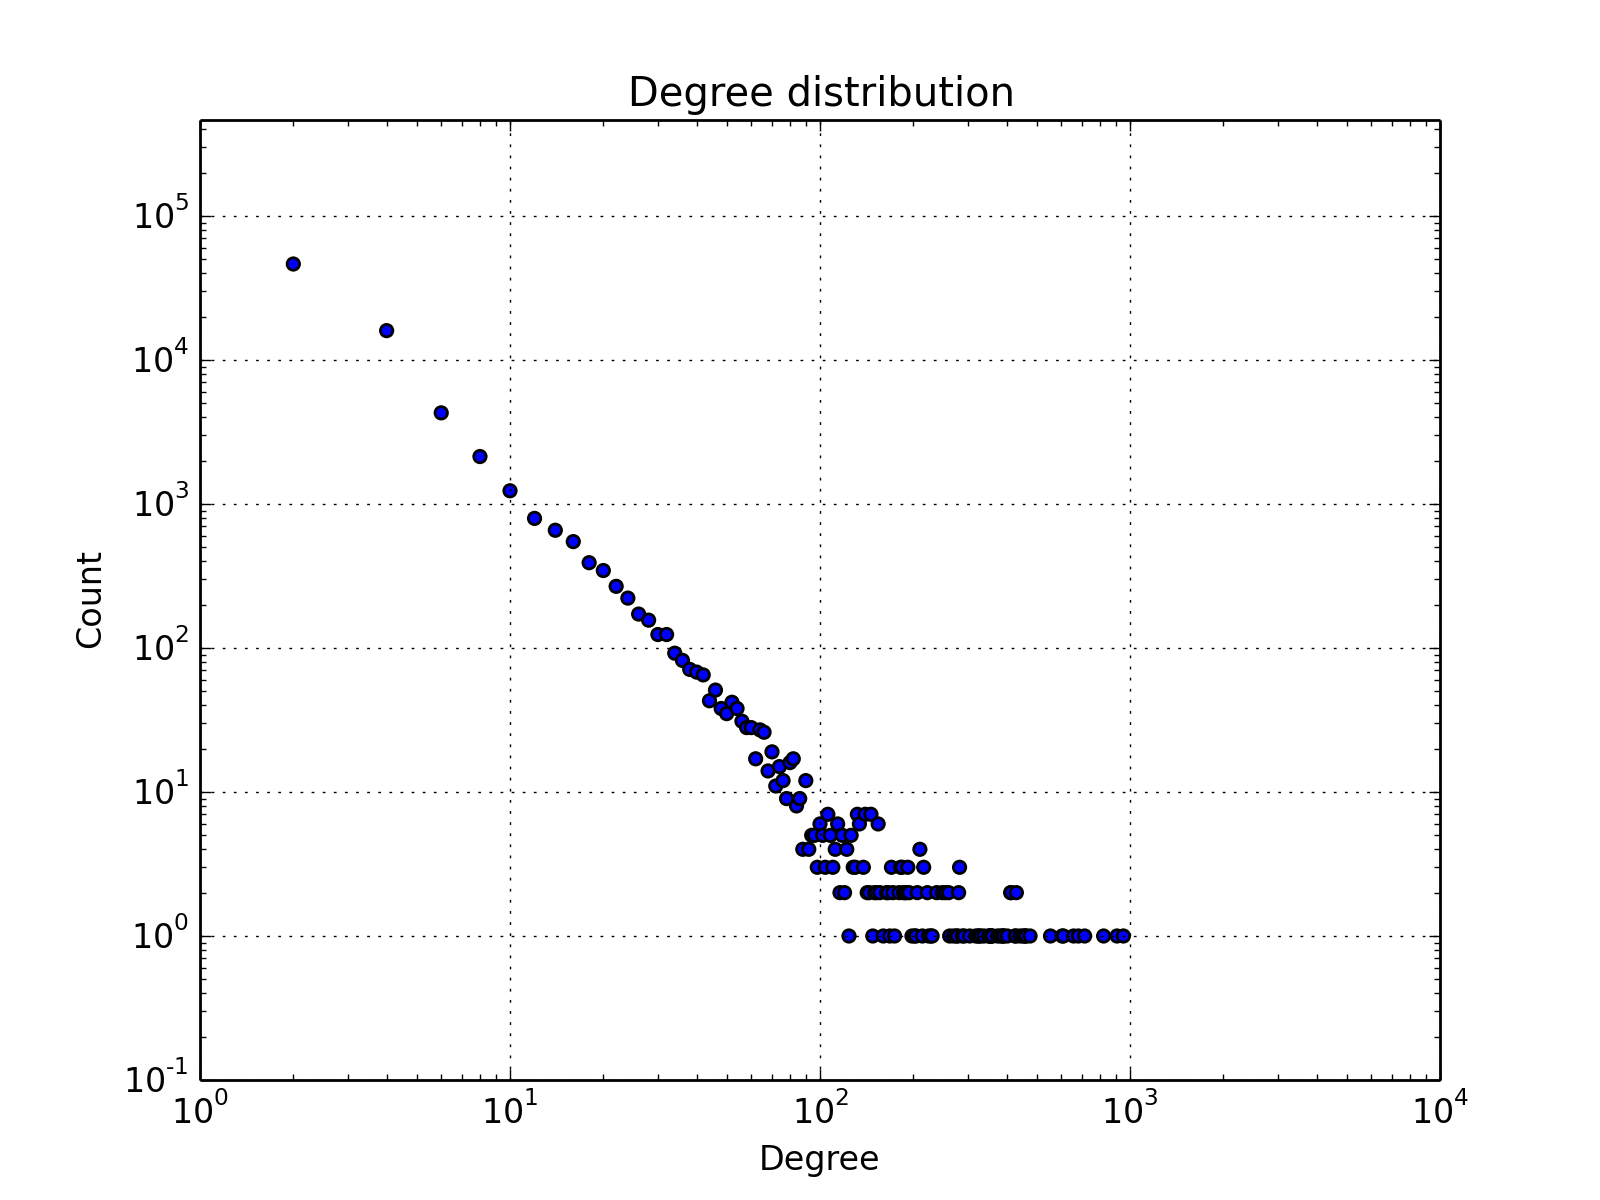
\includegraphics[width=0.35\textwidth]{FIG/DegreeDistoutput_as-skitter.png} 
     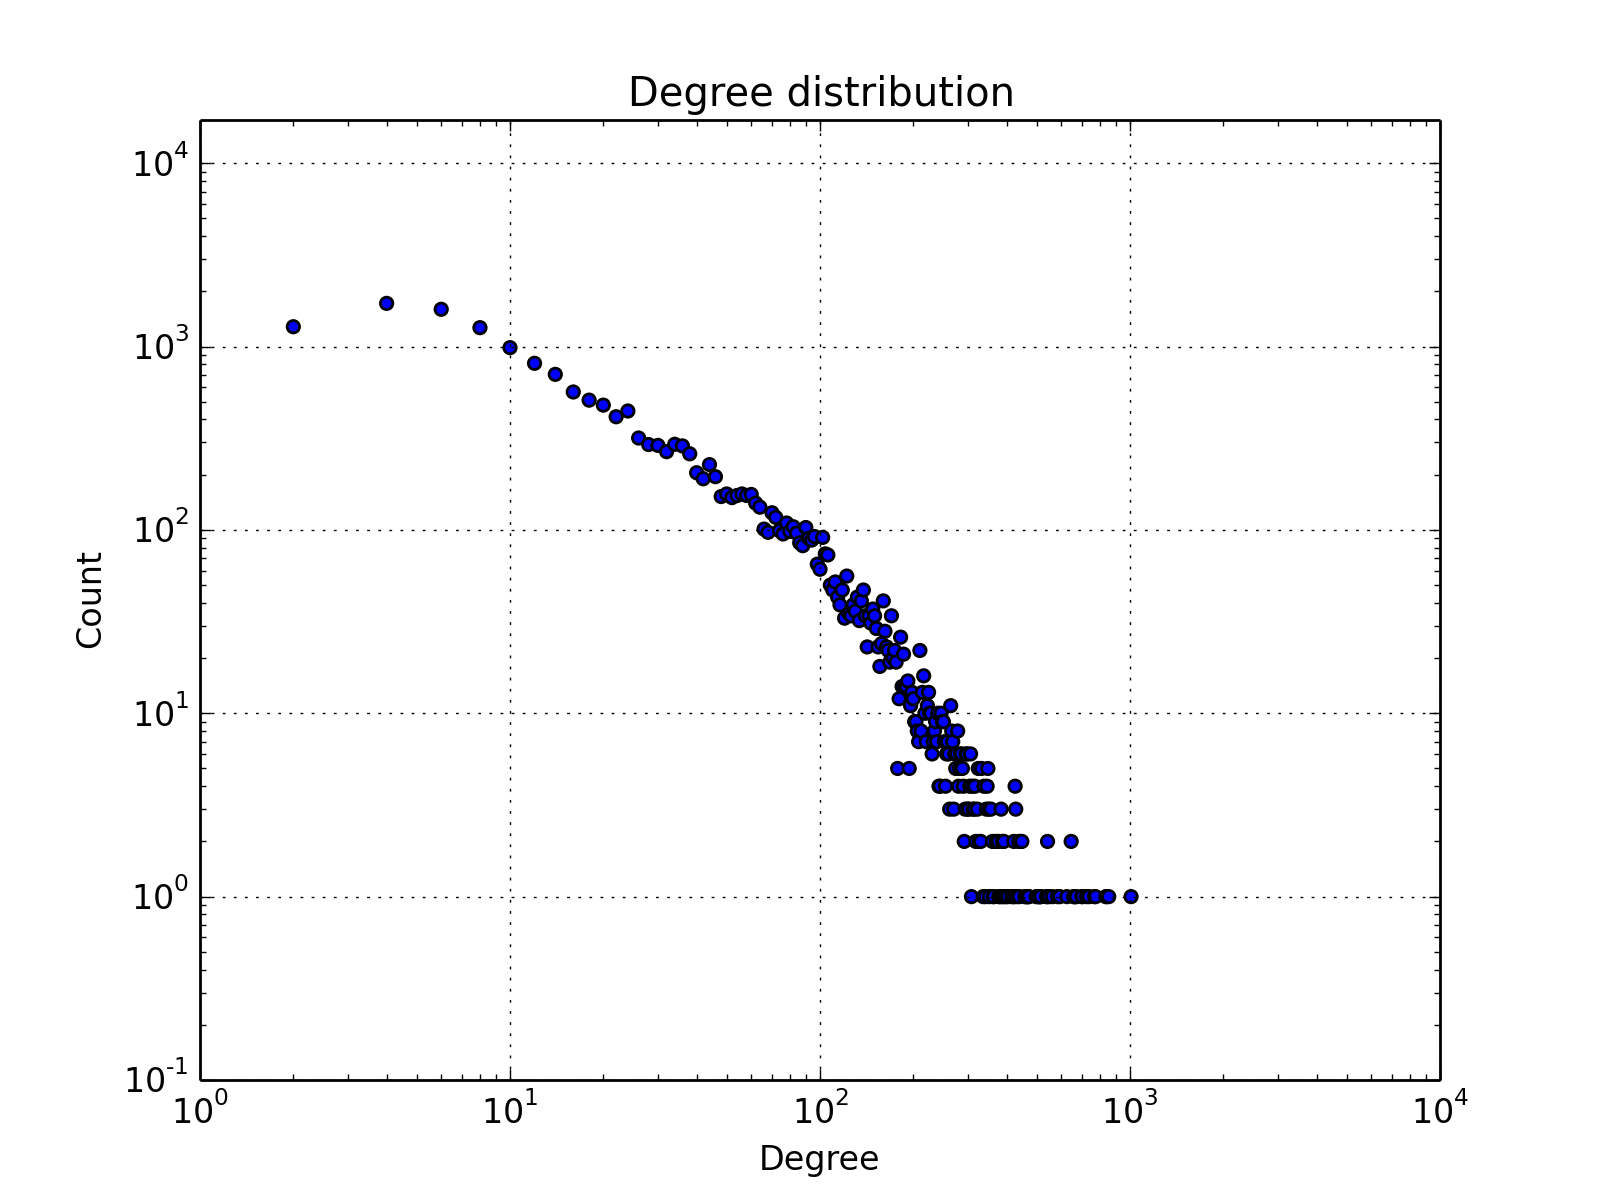
\includegraphics[width=0.35\textwidth]{FIG/DegreeDistoutput_ca-AstroPh.png}
     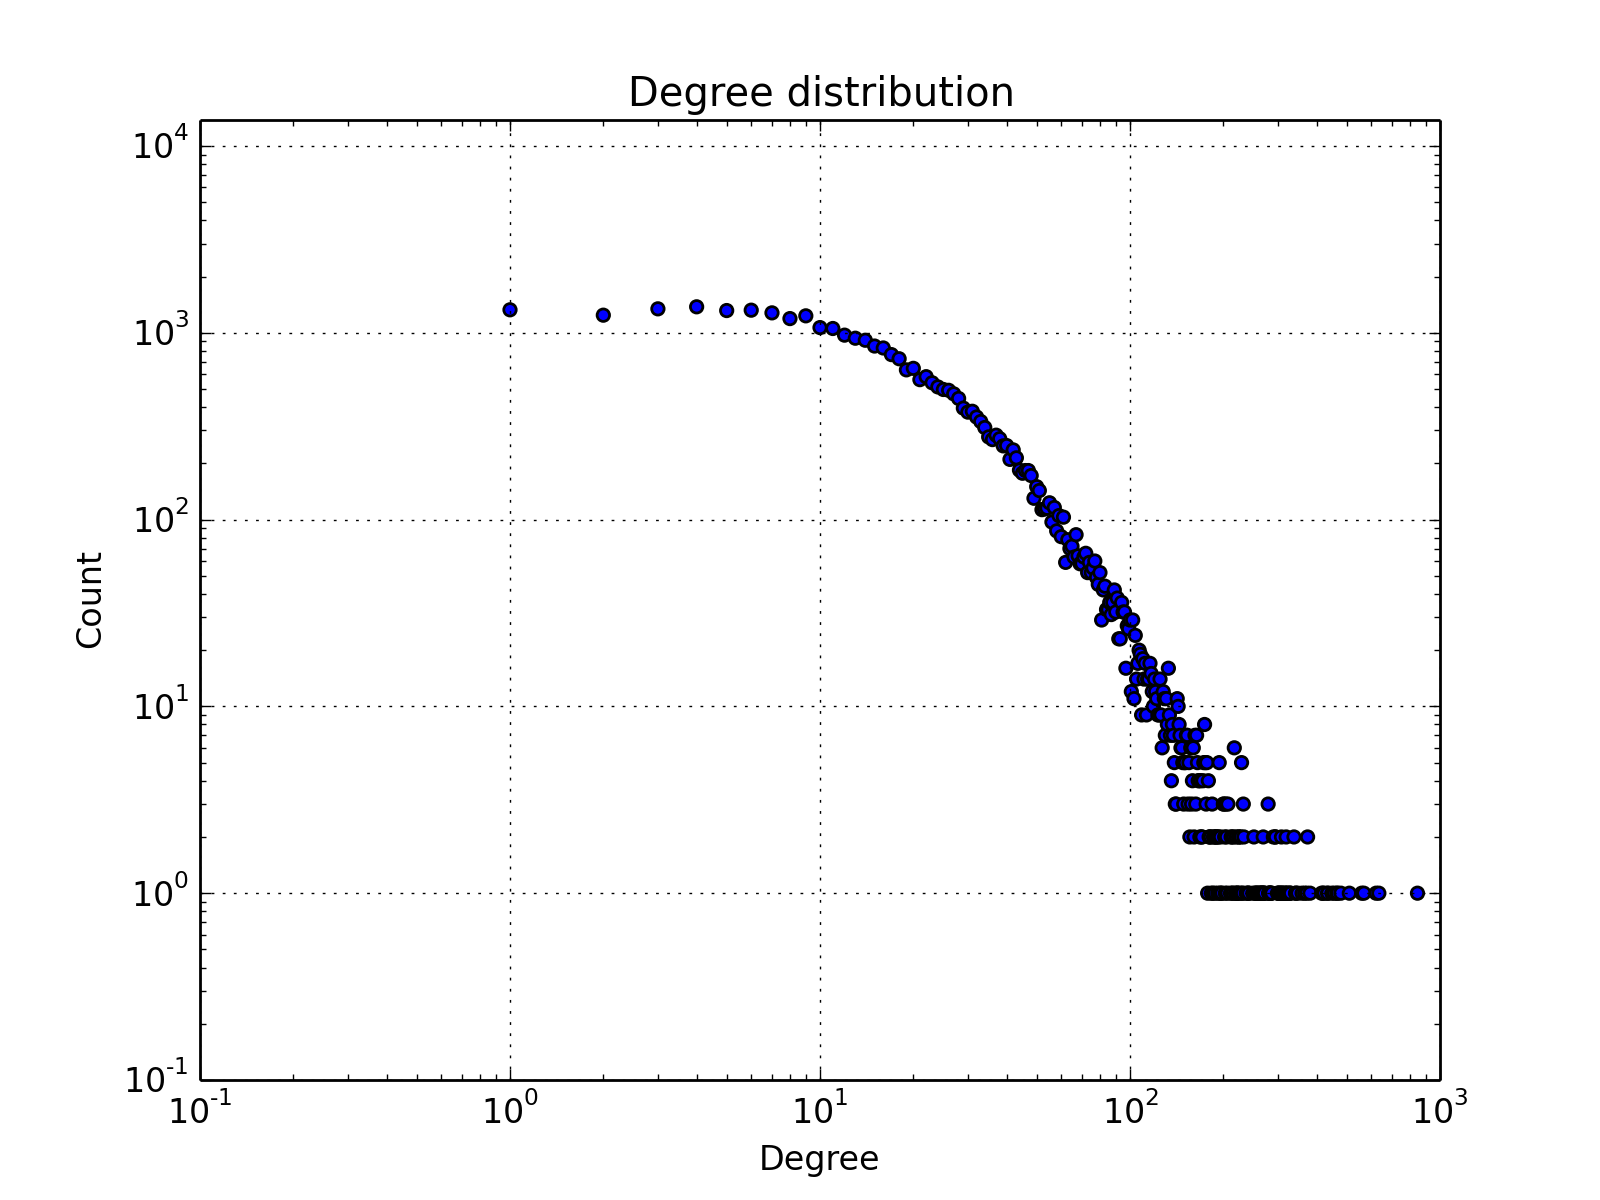
\includegraphics[width=0.35\textwidth]{FIG/DegreeDistoutput_cit-HepPh.png} \\
     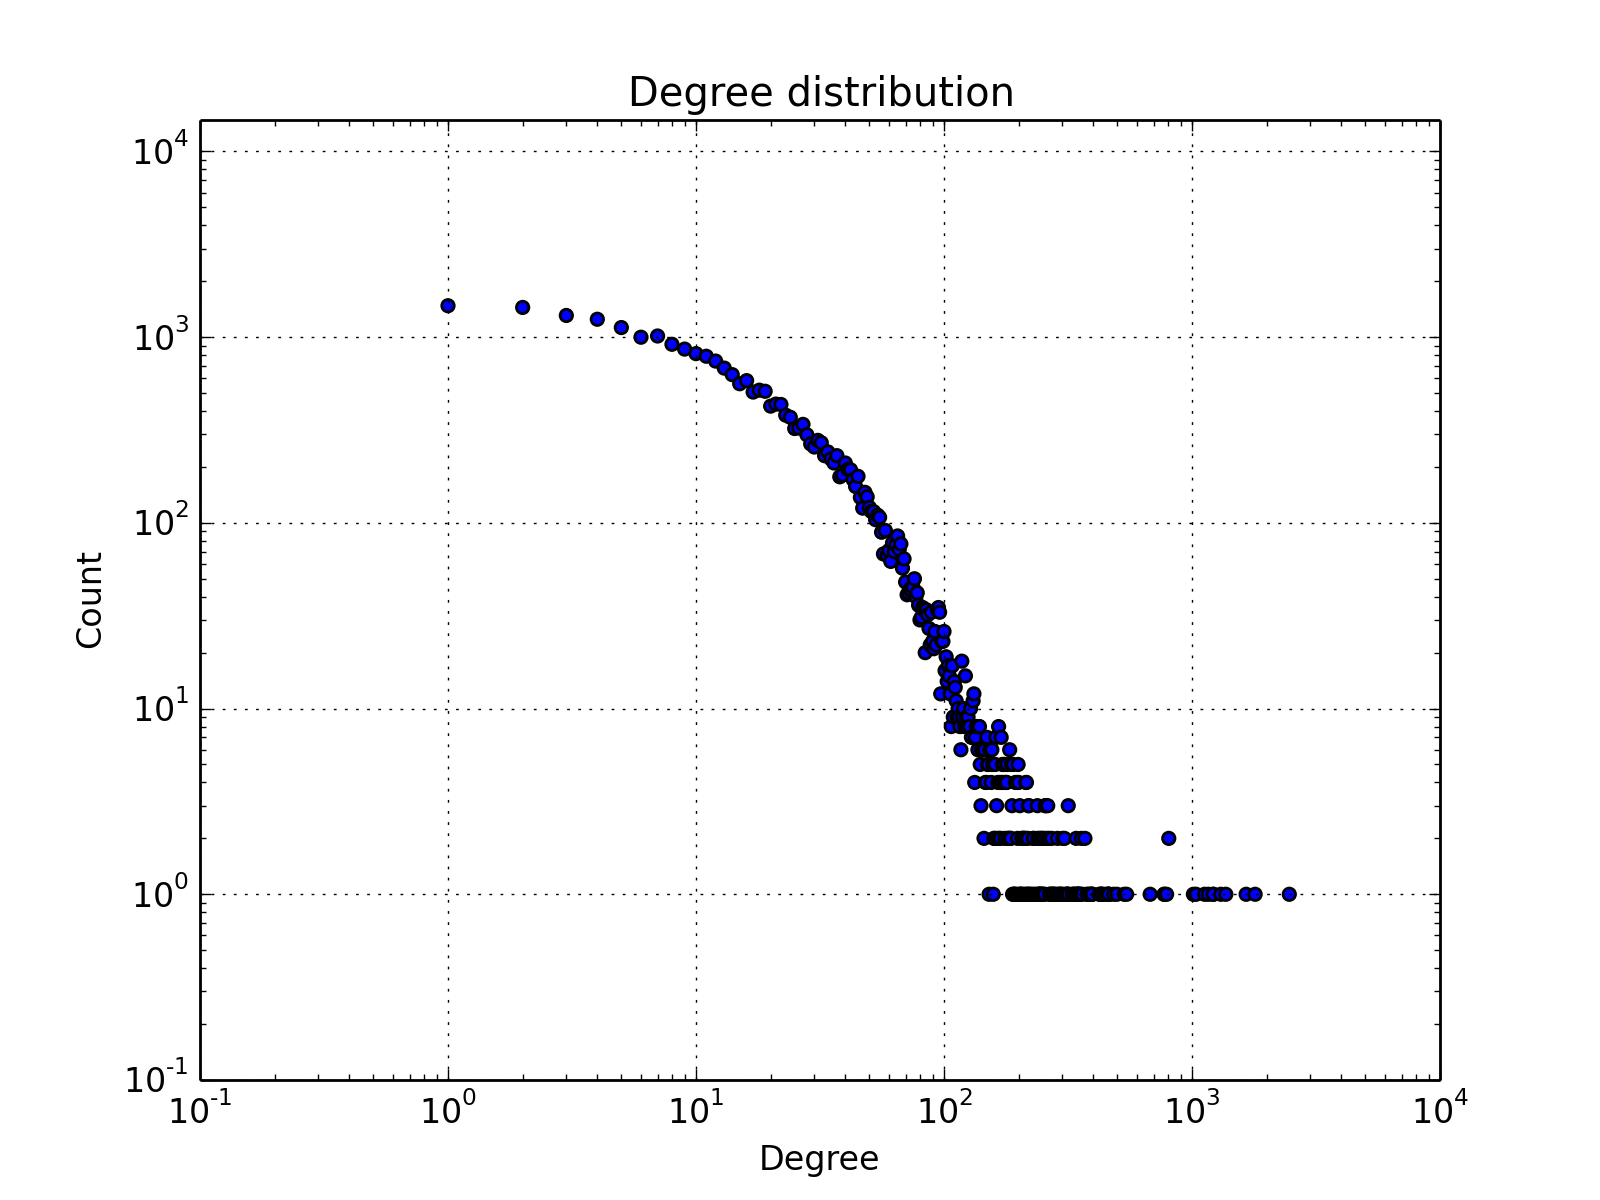
\includegraphics[width=0.35\textwidth]{FIG/DegreeDistoutput_cit-HepTh.png} 
     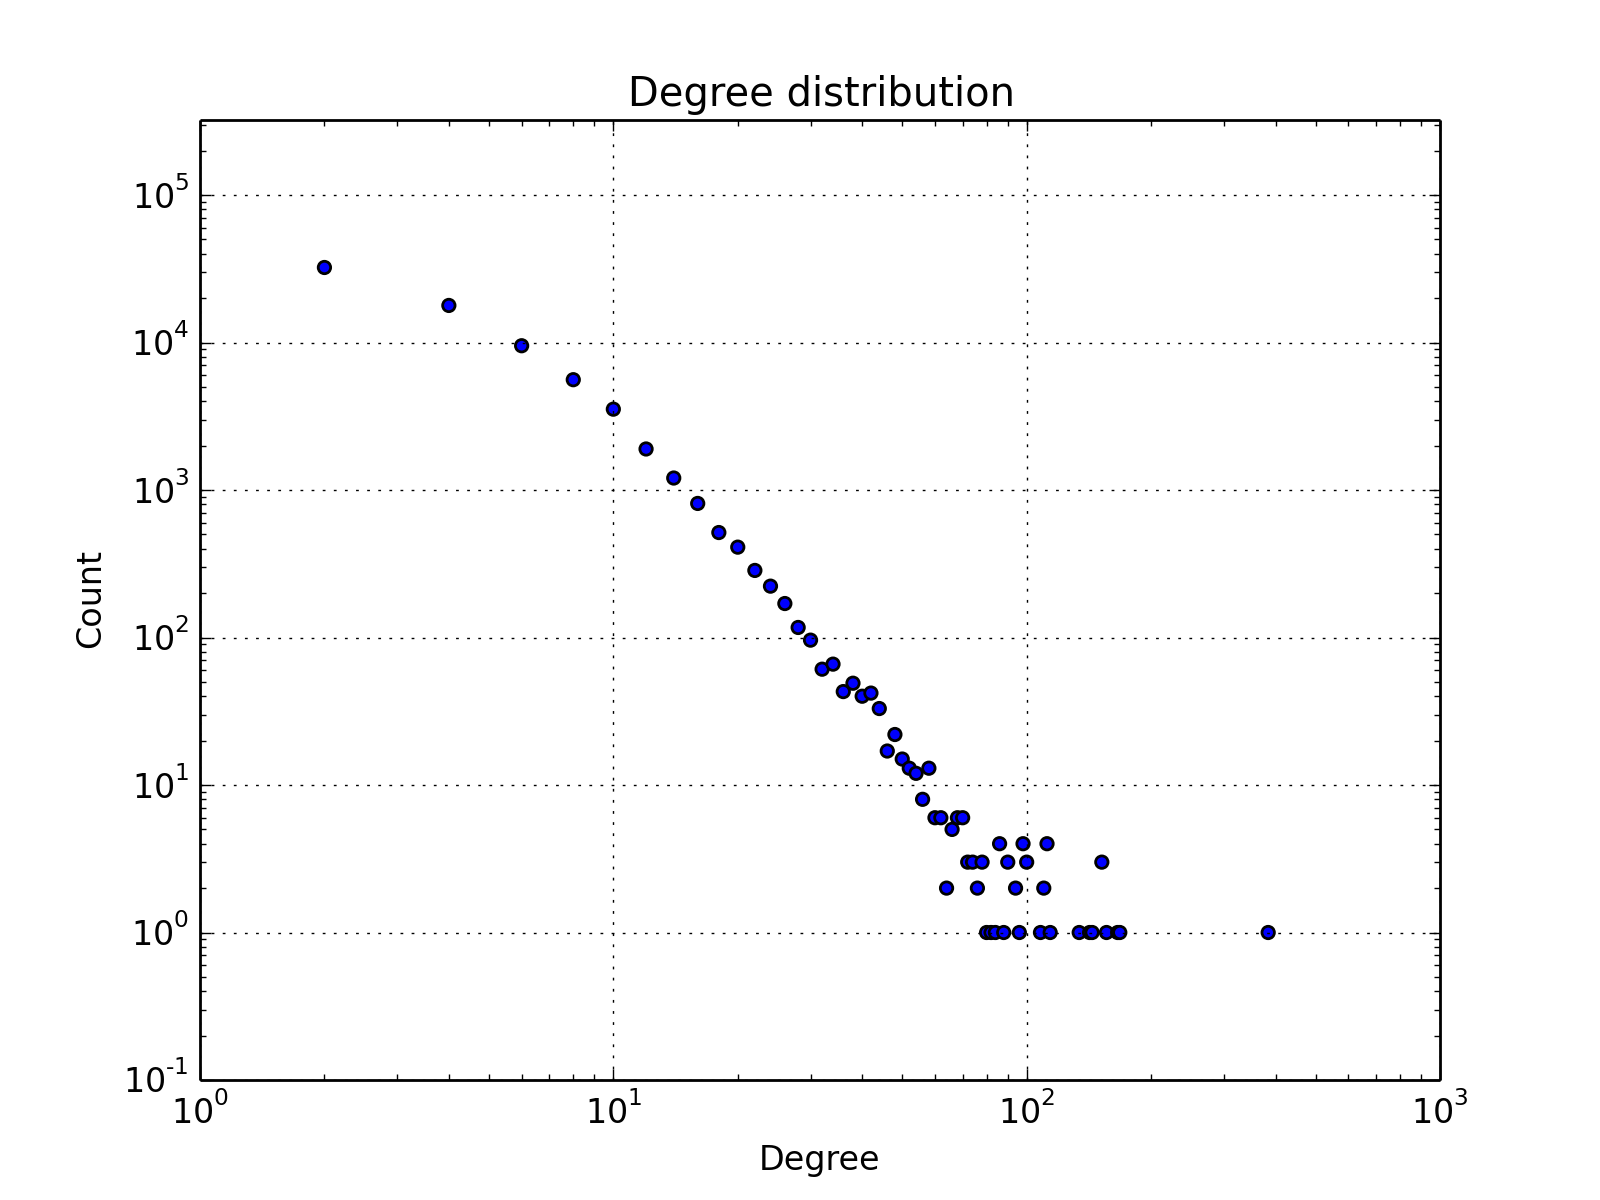
\includegraphics[width=0.35\textwidth]{FIG/DegreeDistoutput_com-amazon.png} 
     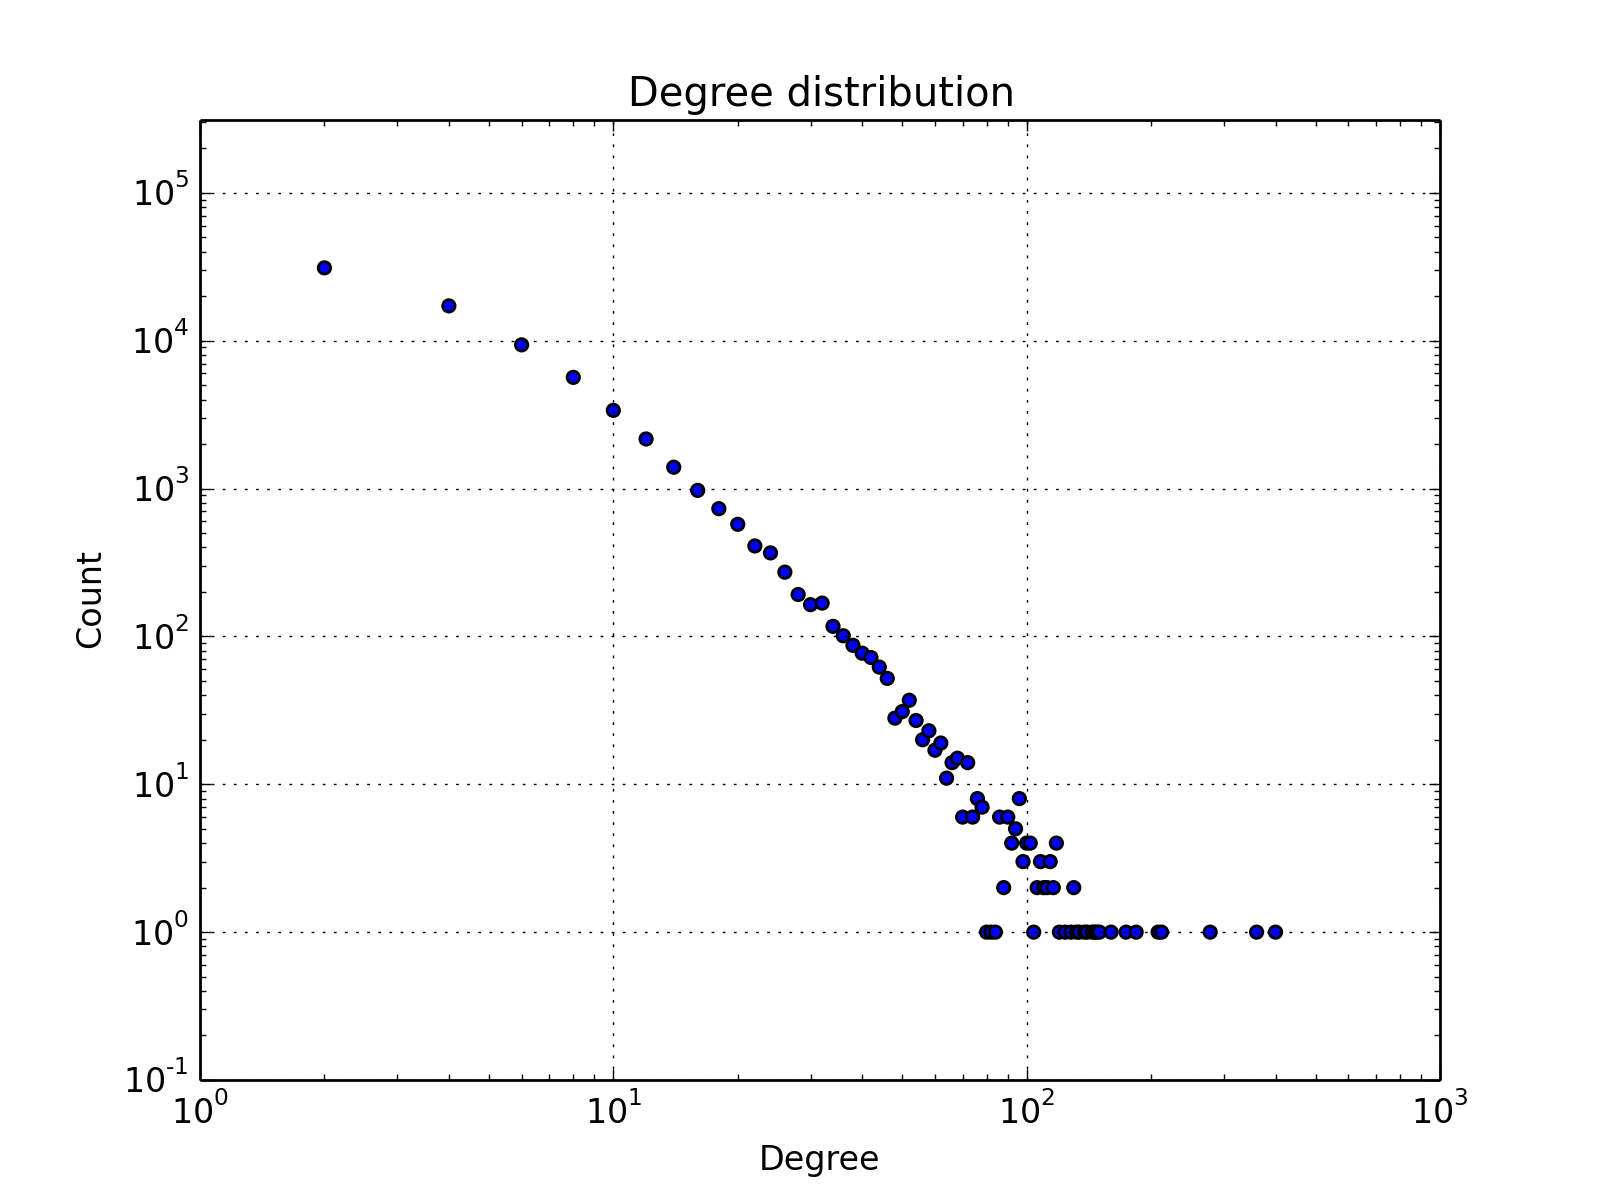
\includegraphics[width=0.35\textwidth]{FIG/DegreeDistoutput_com-dblp.png} \\
     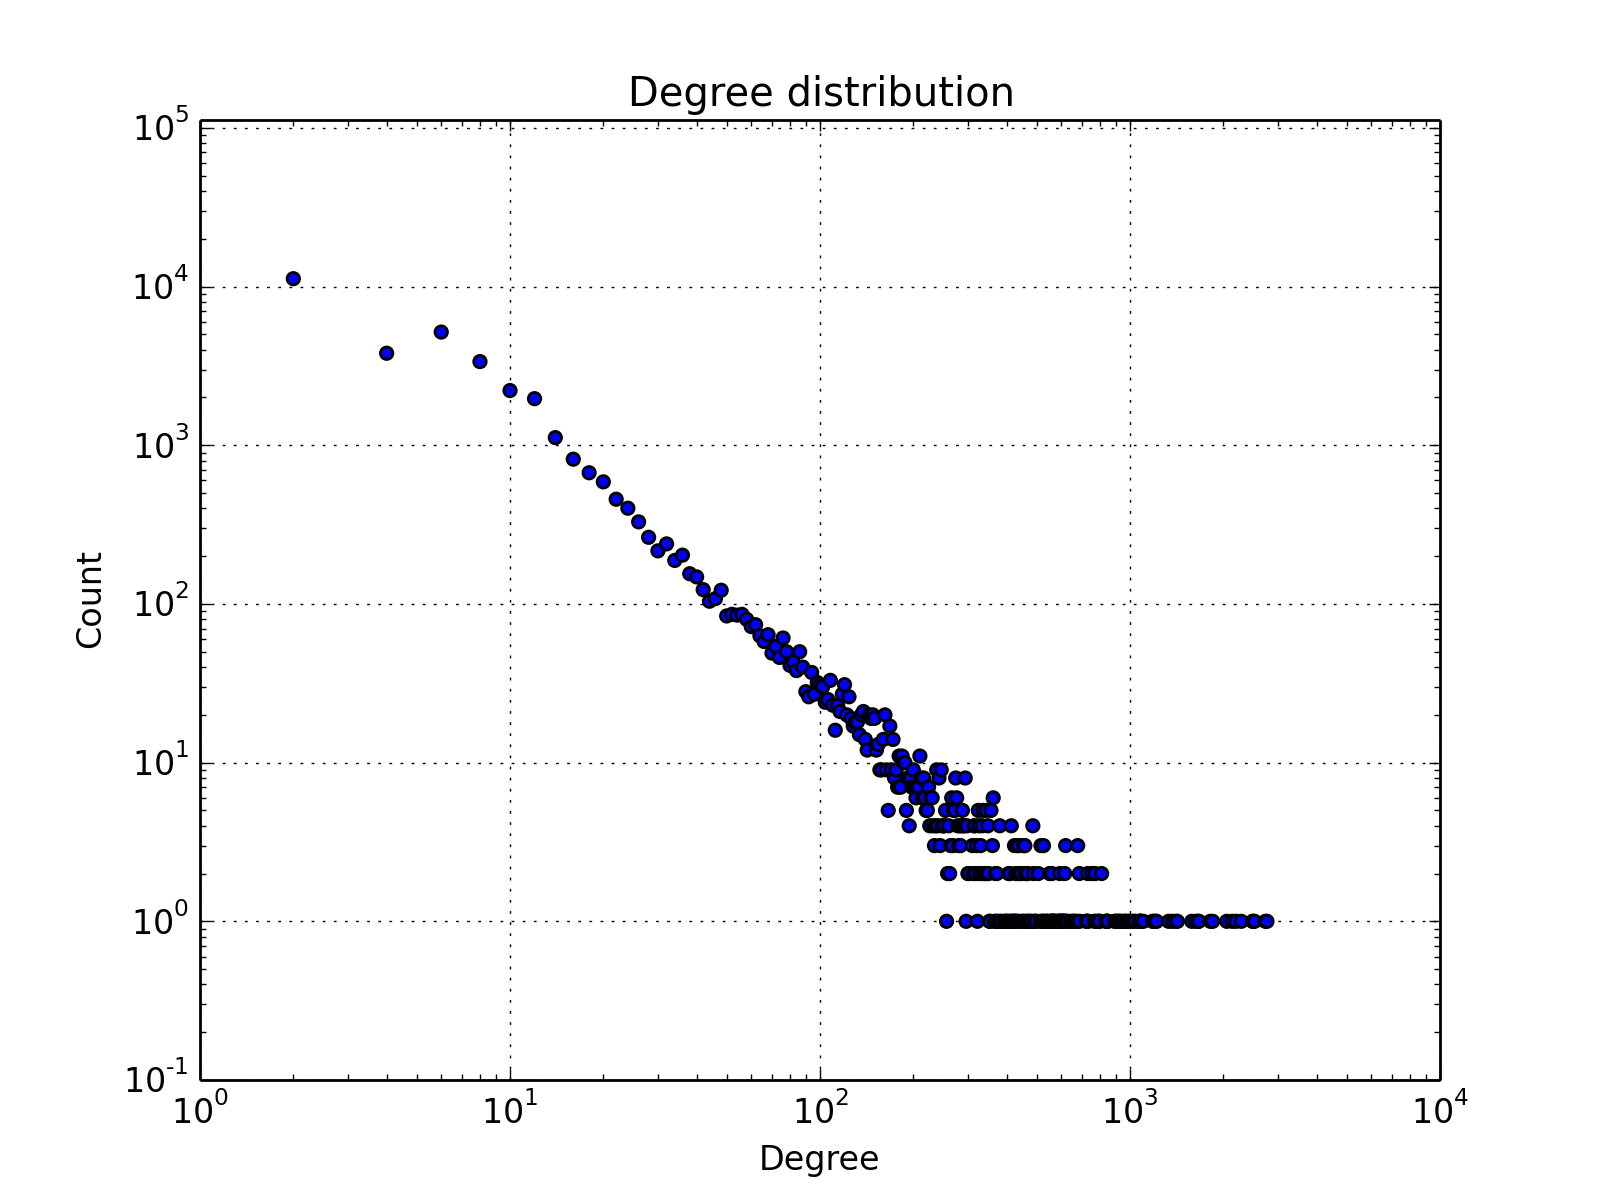
\includegraphics[width=0.35\textwidth]{FIG/DegreeDistoutput_email-Enron.png} 
     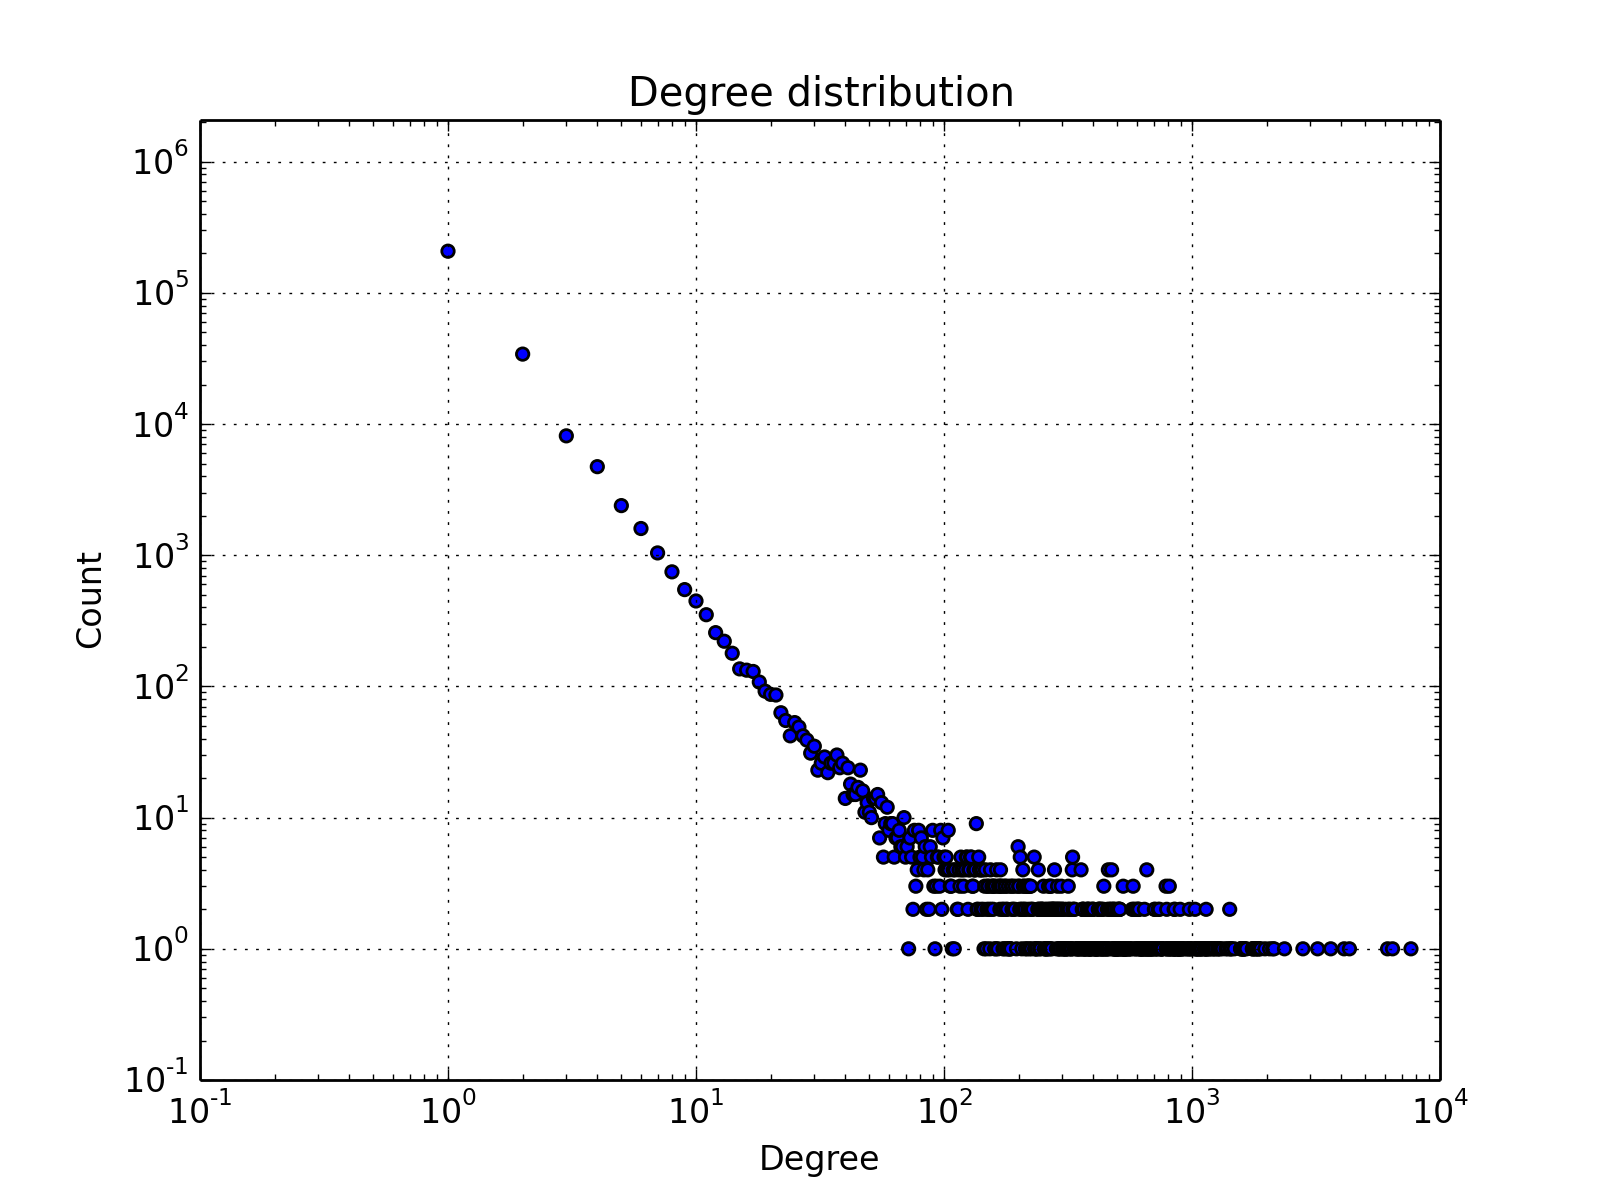
\includegraphics[width=0.35\textwidth]{FIG/DegreeDistoutput_email-EuAll.png} 
     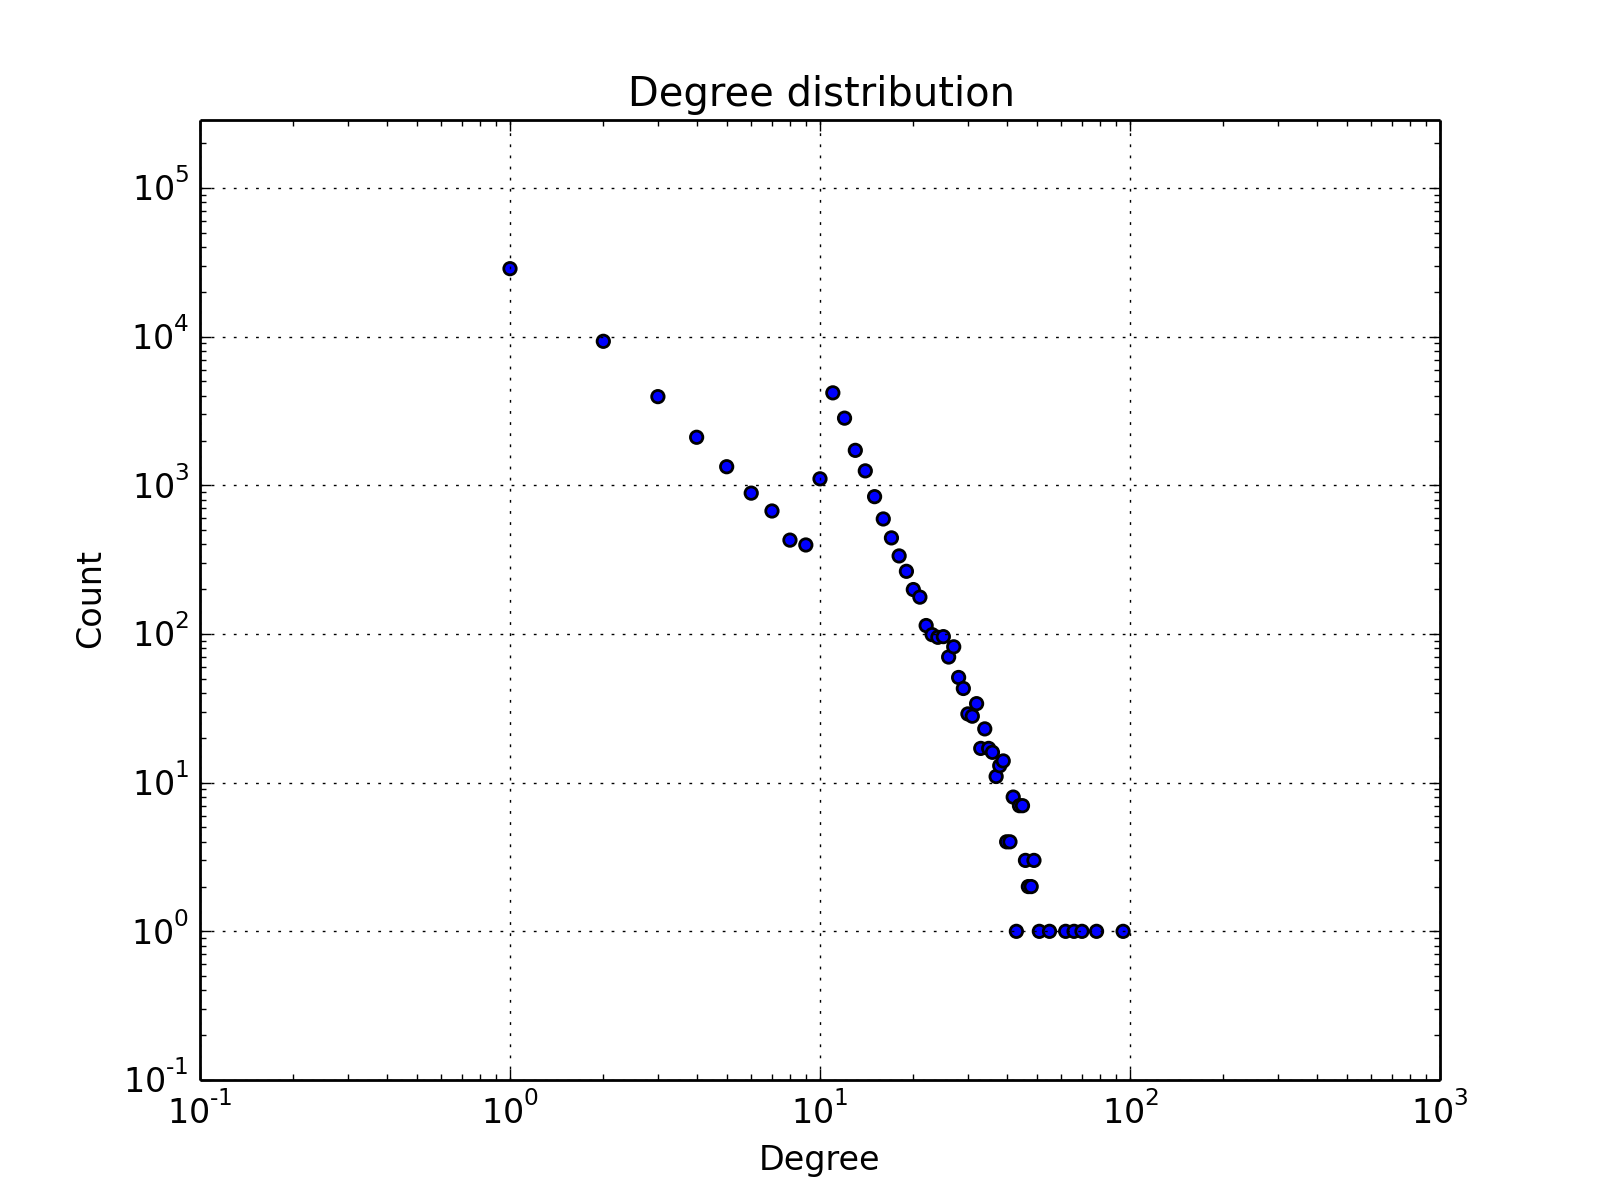
\includegraphics[width=0.35\textwidth]{FIG/DegreeDistoutput_p2p-Gnutella31.png} \\
     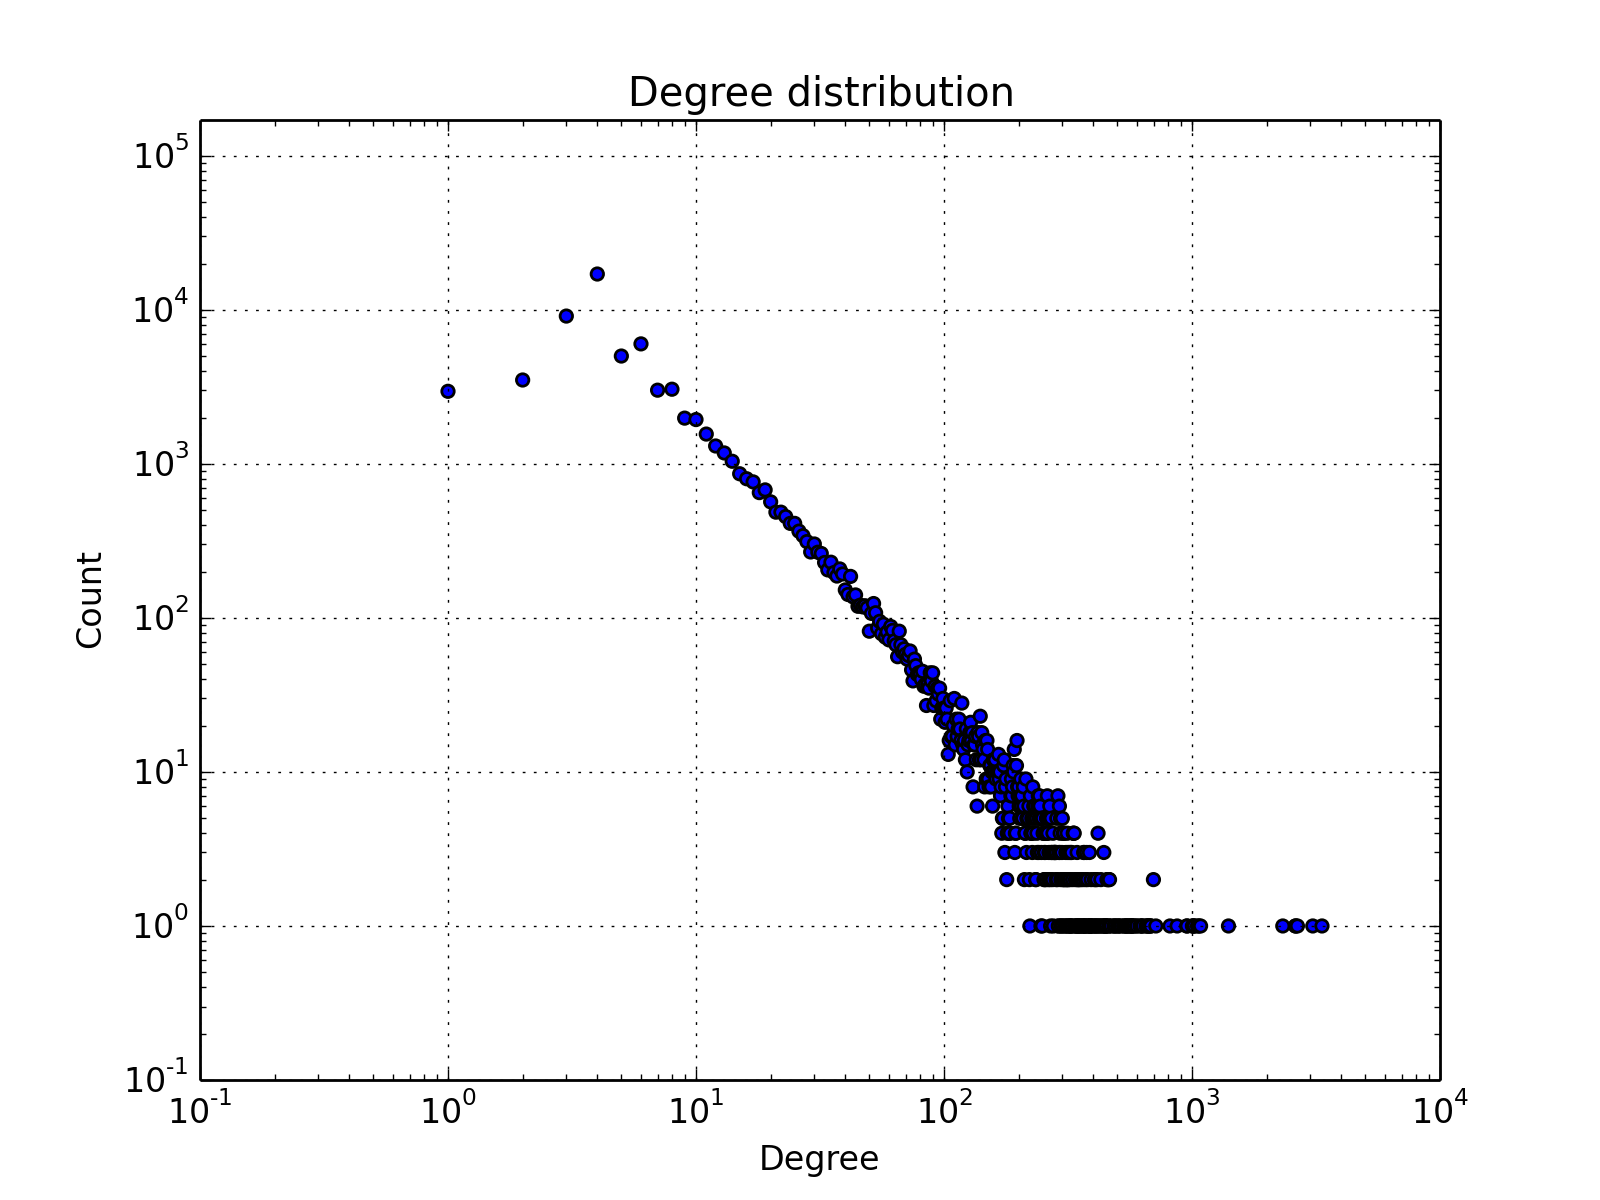
\includegraphics[width=0.35\textwidth]{FIG/DegreeDistoutput_soc-Slashdot0811-75000.png} 
\end{tabular}
\caption{Degree distribution plots of 10 graphs}
\label{fig:results}
\end{center}
\end{figure}

For 6 directed graphs out of all 10 graphs, we can also plot Indegree vs. Count and Outdegree vs. Count in log space

\begin{figure}[H]
\begin{center}
\begin{tabular}{ccc}
     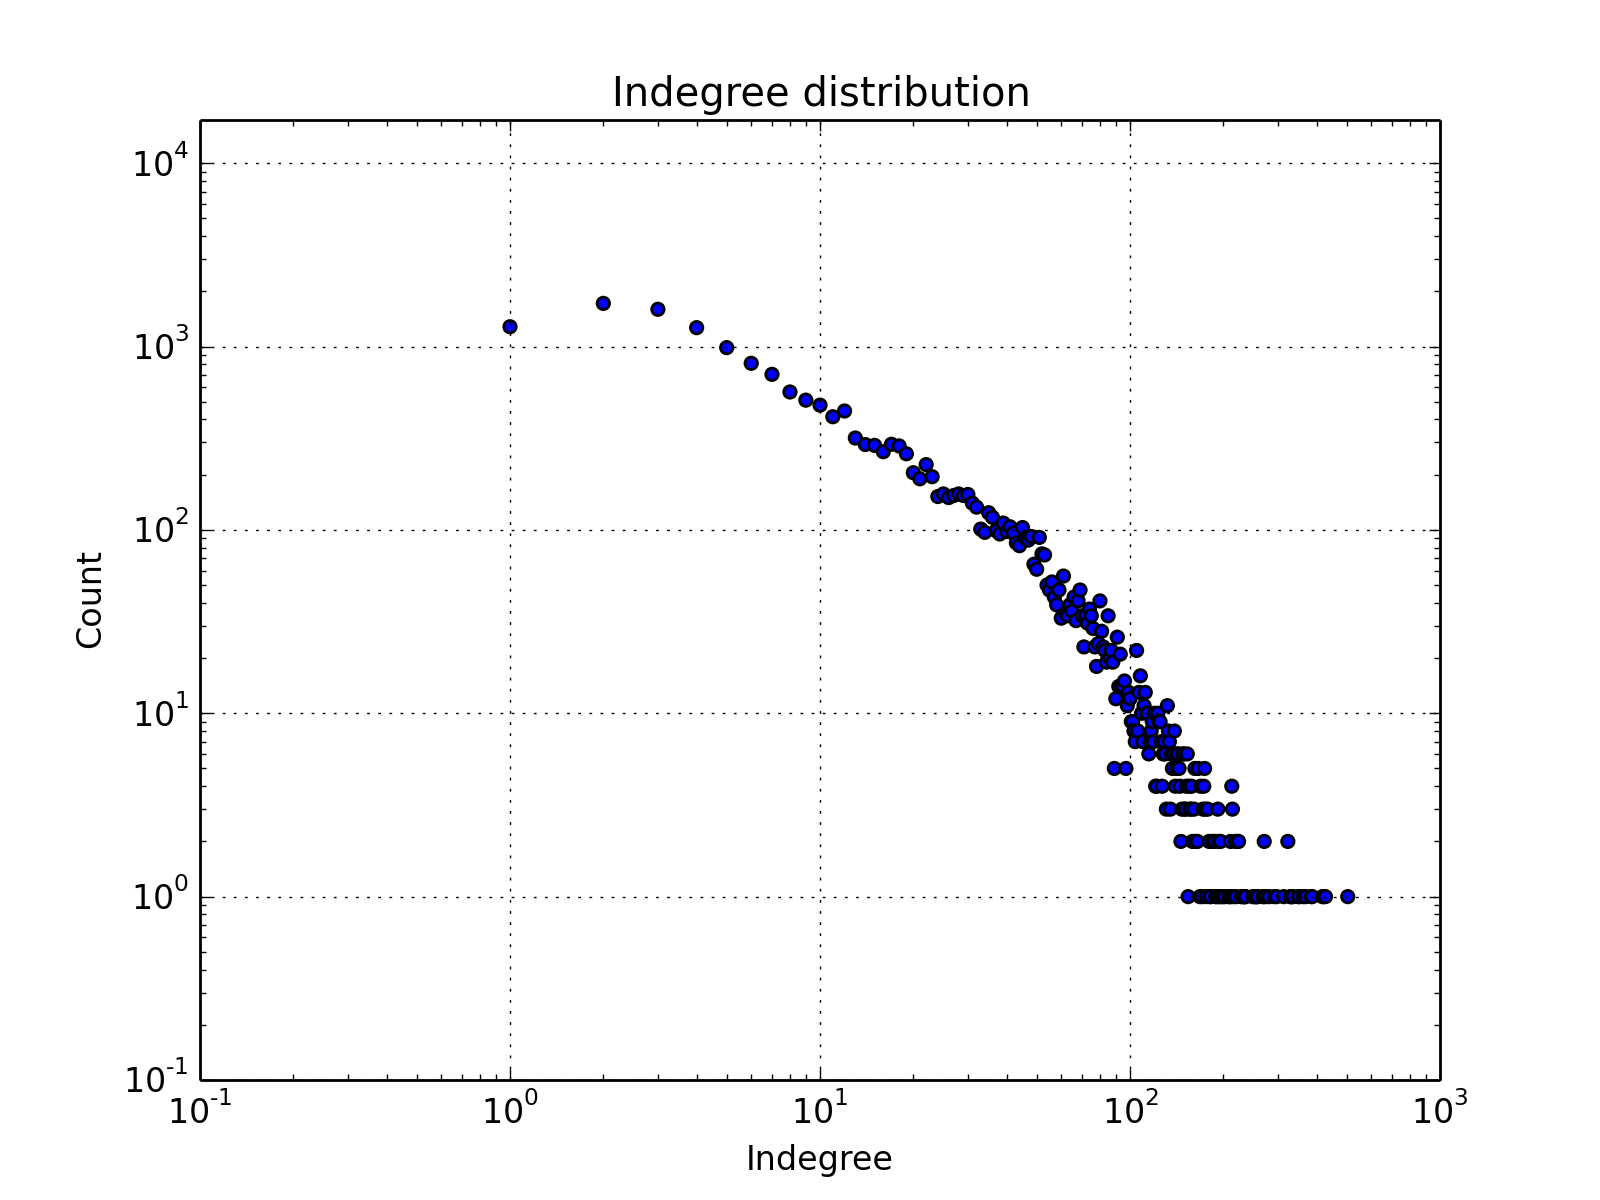
\includegraphics[width=0.35\textwidth]{FIG/IndegreeDistoutput_ca-AstroPh.png}
     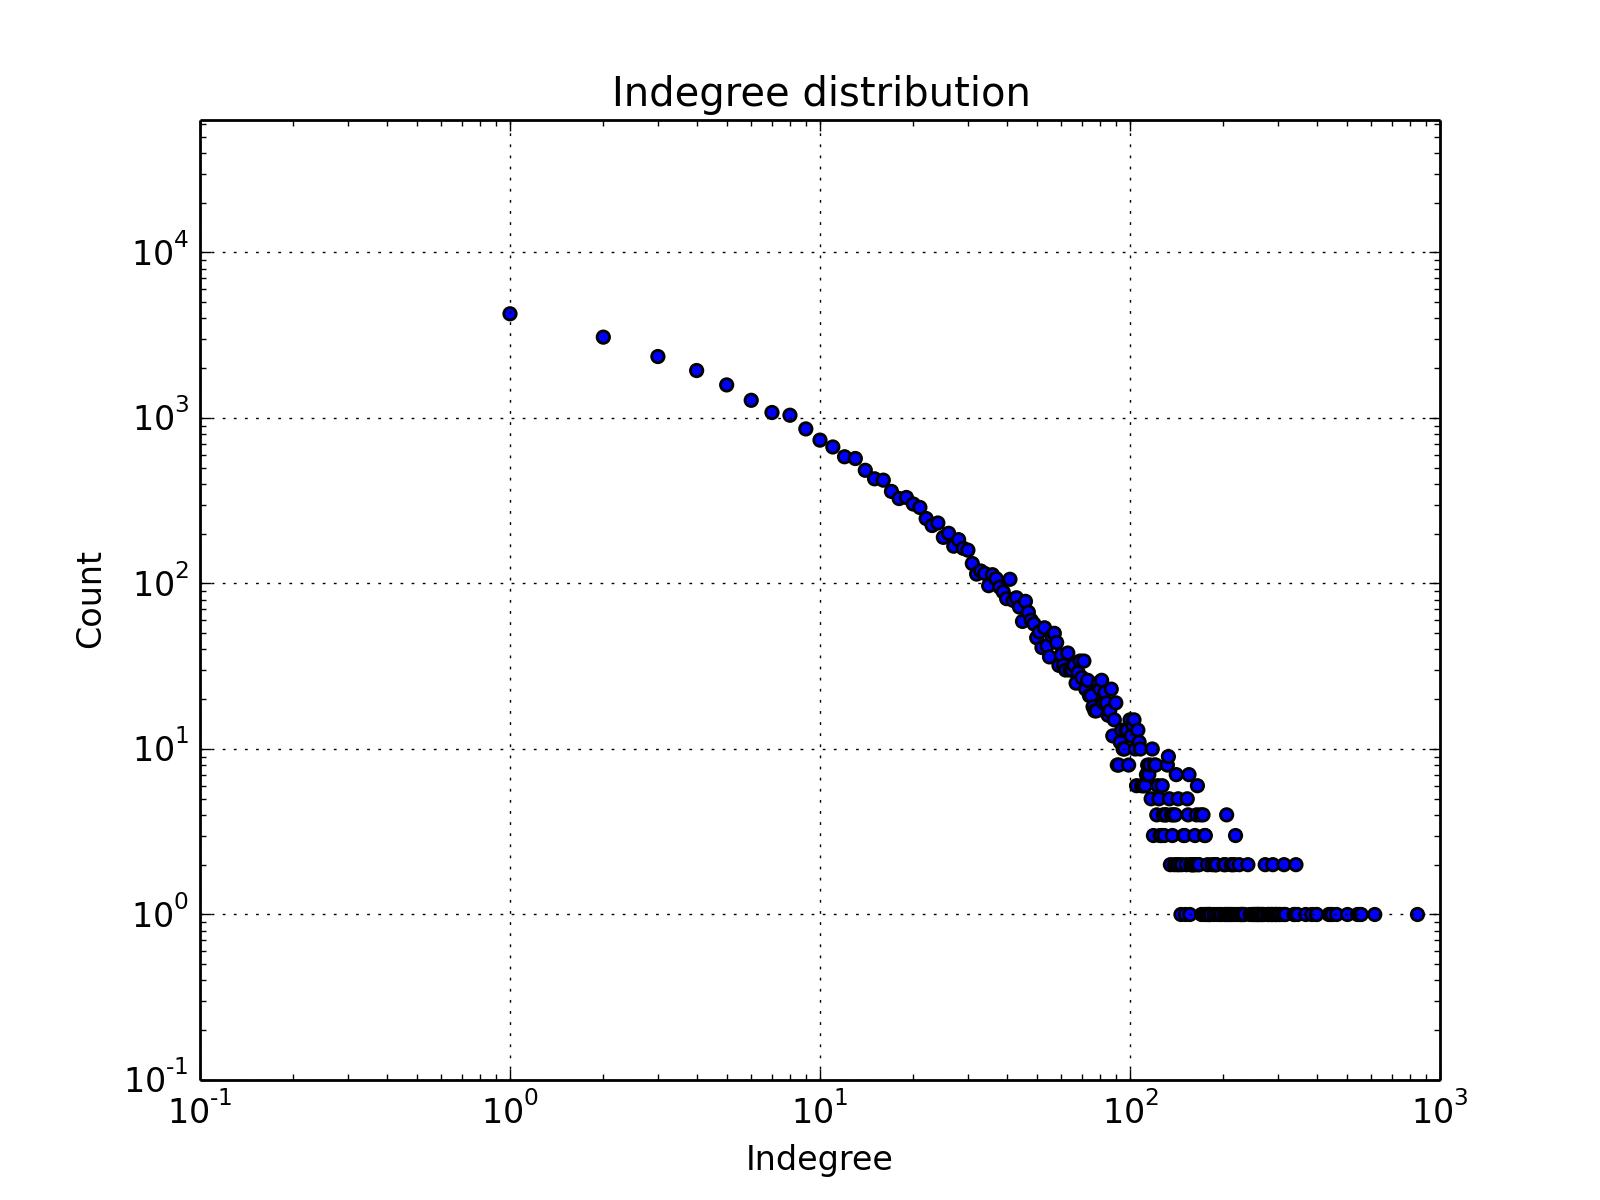
\includegraphics[width=0.35\textwidth]{FIG/IndegreeDistoutput_cit-HepPh.png} 
     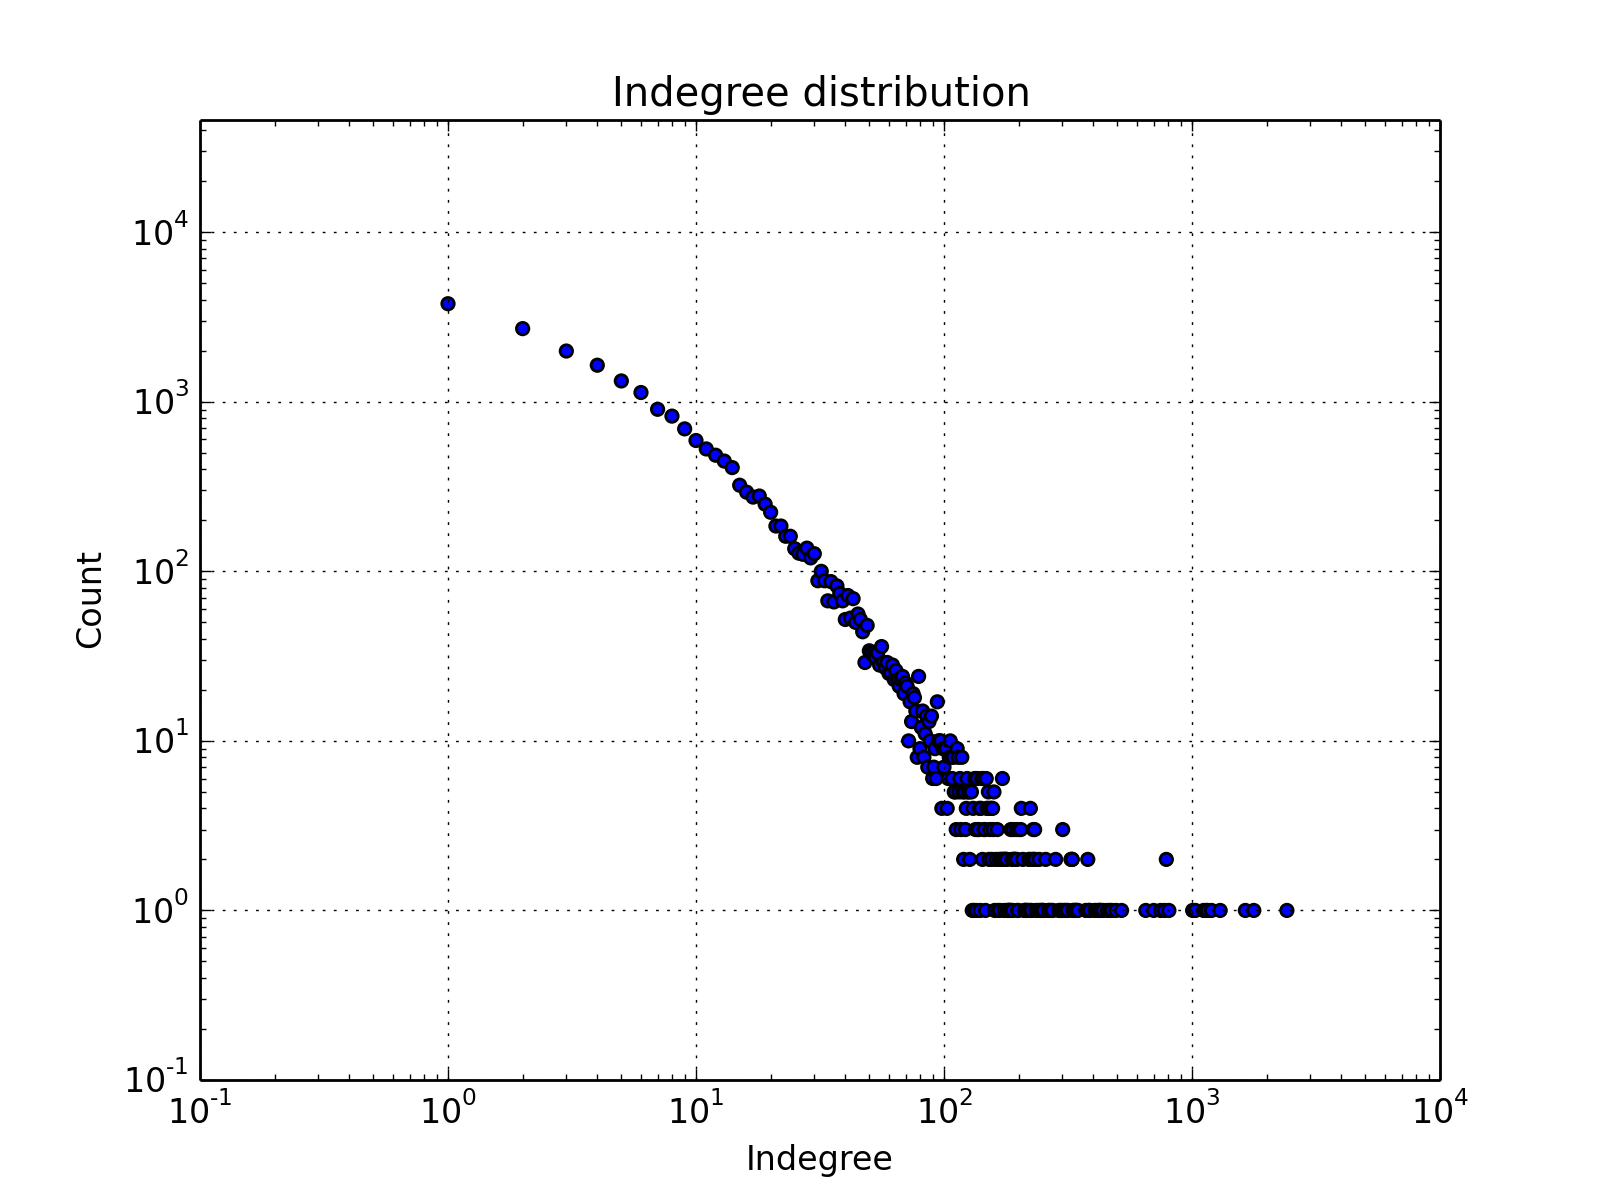
\includegraphics[width=0.35\textwidth]{FIG/IndegreeDistoutput_cit-HepTh.png} \\
     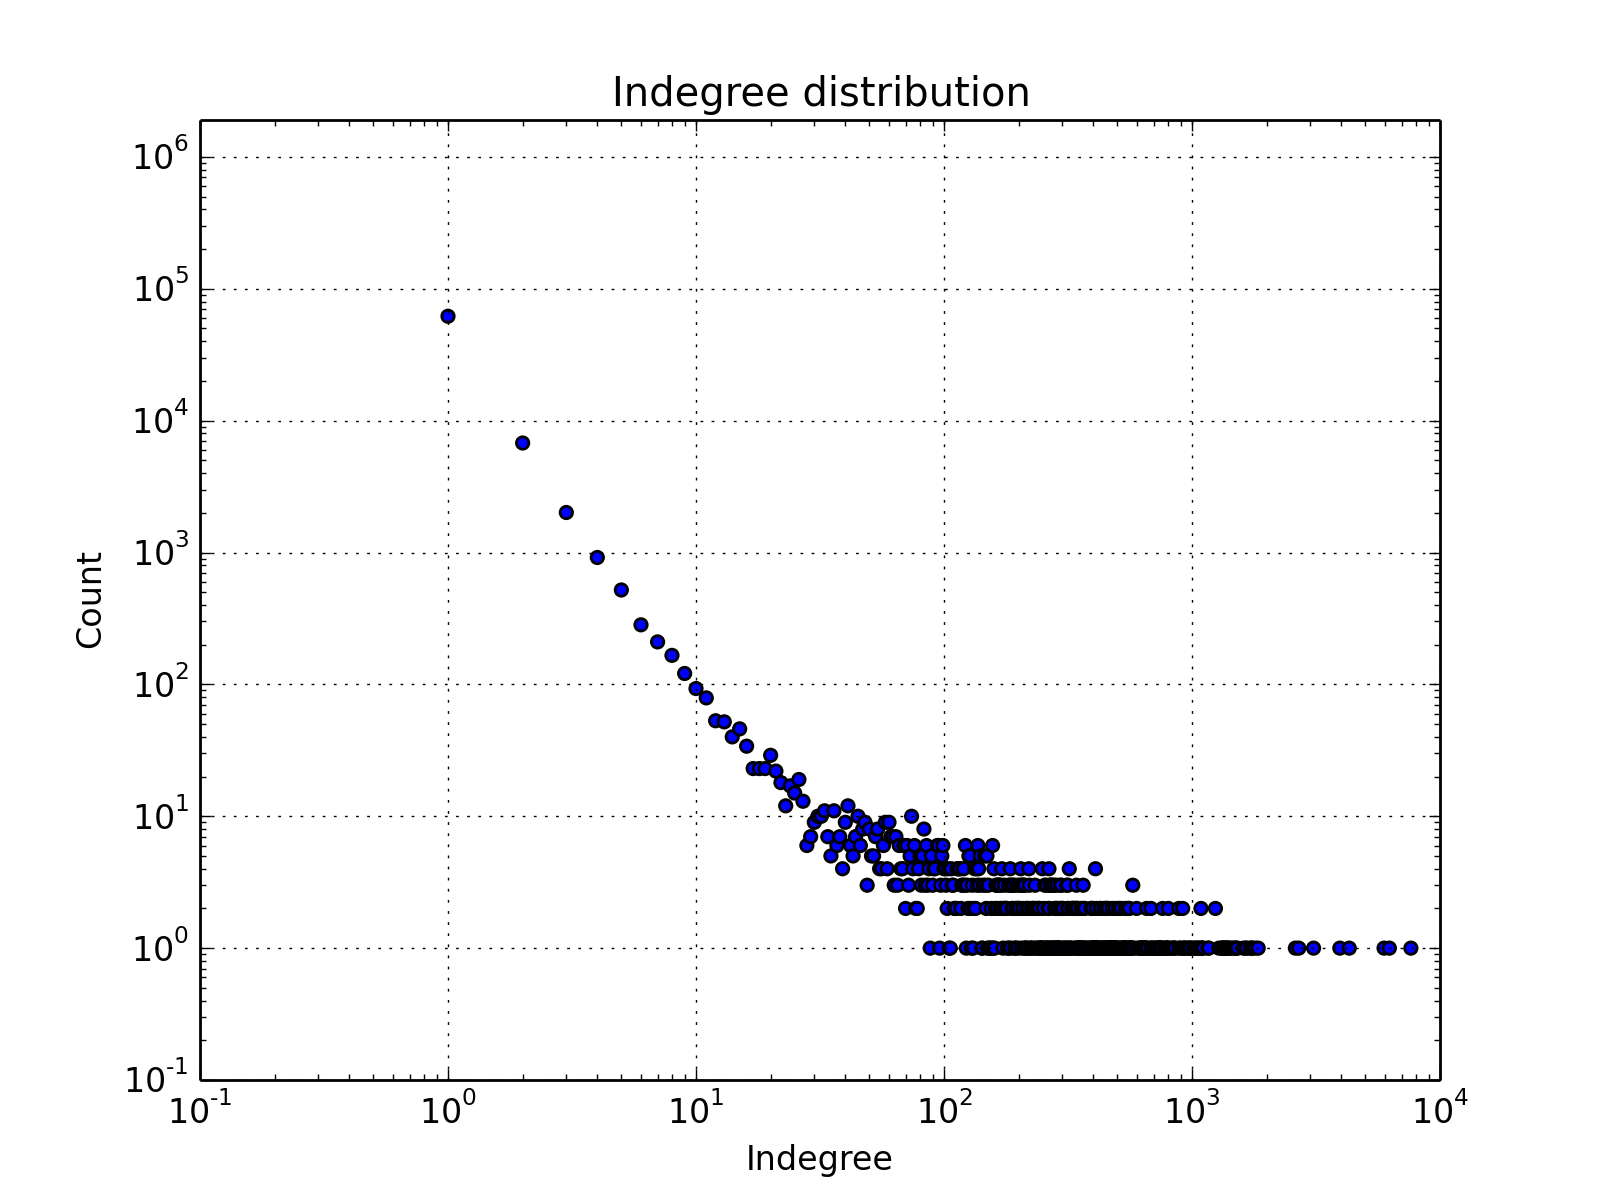
\includegraphics[width=0.35\textwidth]{FIG/IndegreeDistoutput_email-EuAll.png} 
     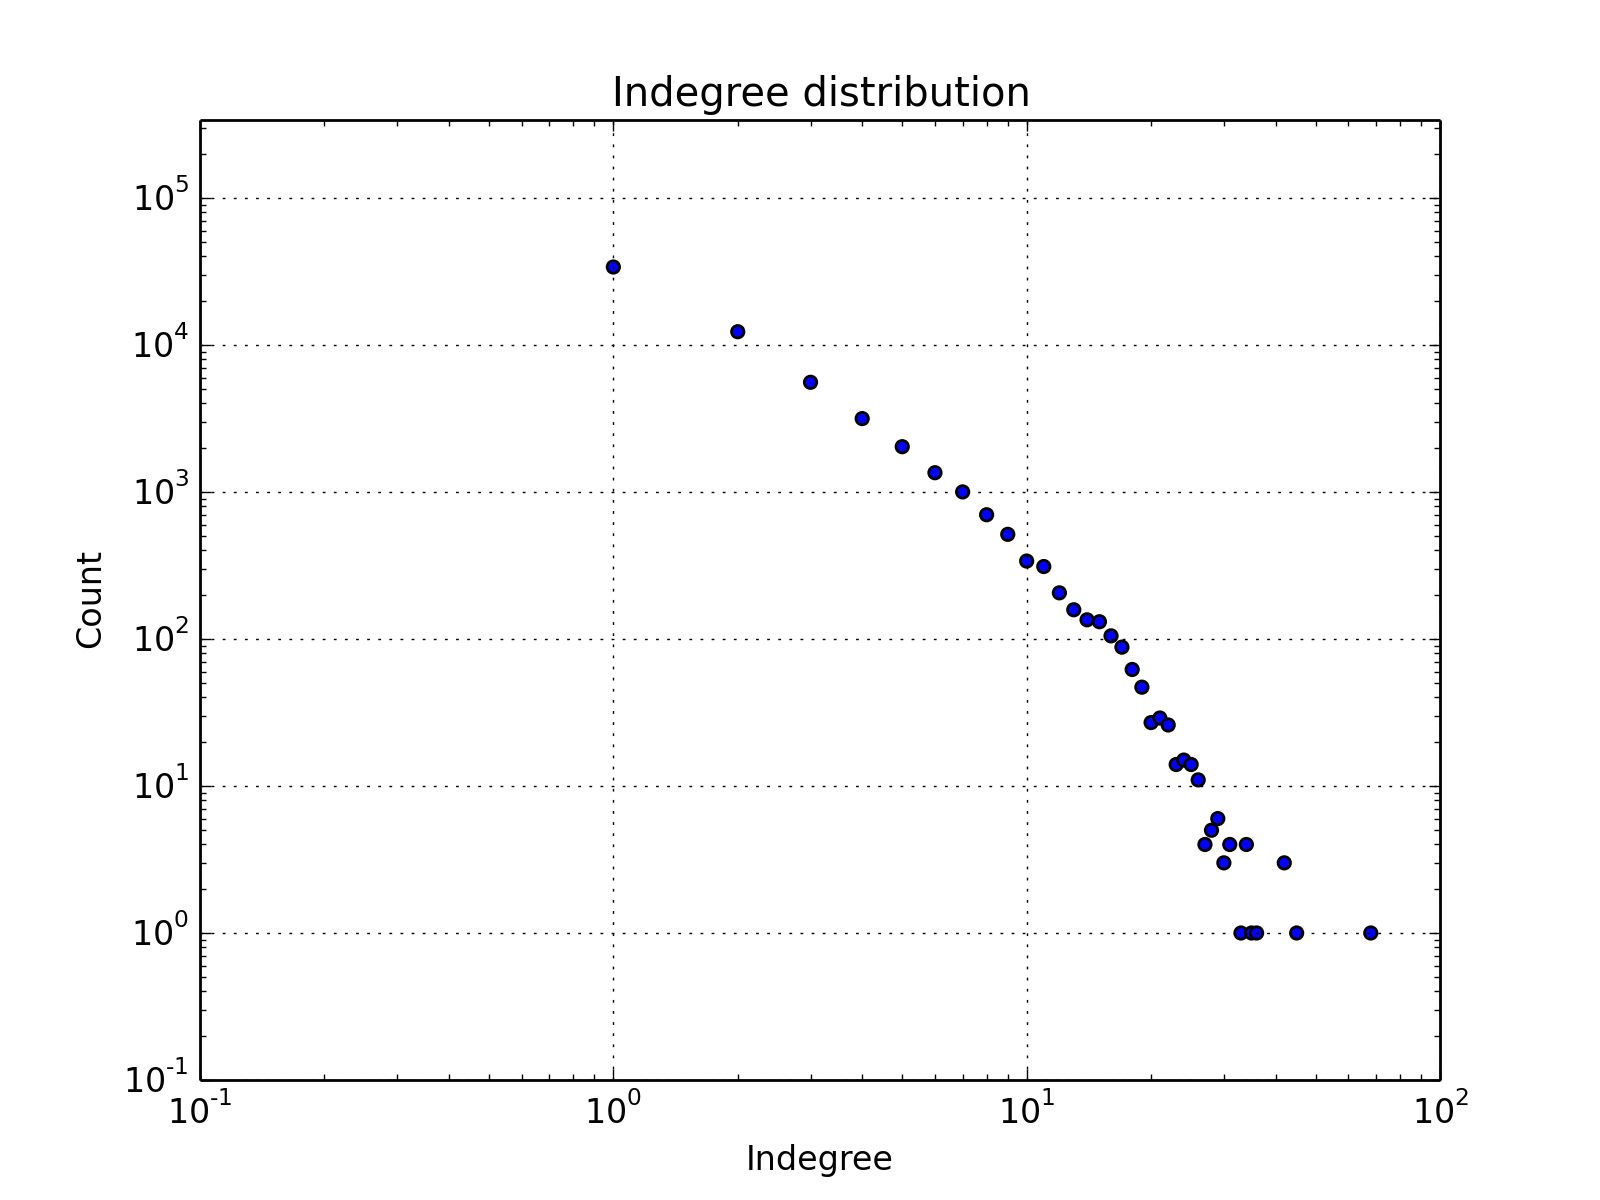
\includegraphics[width=0.35\textwidth]{FIG/IndegreeDistoutput_p2p-Gnutella31.png} 
     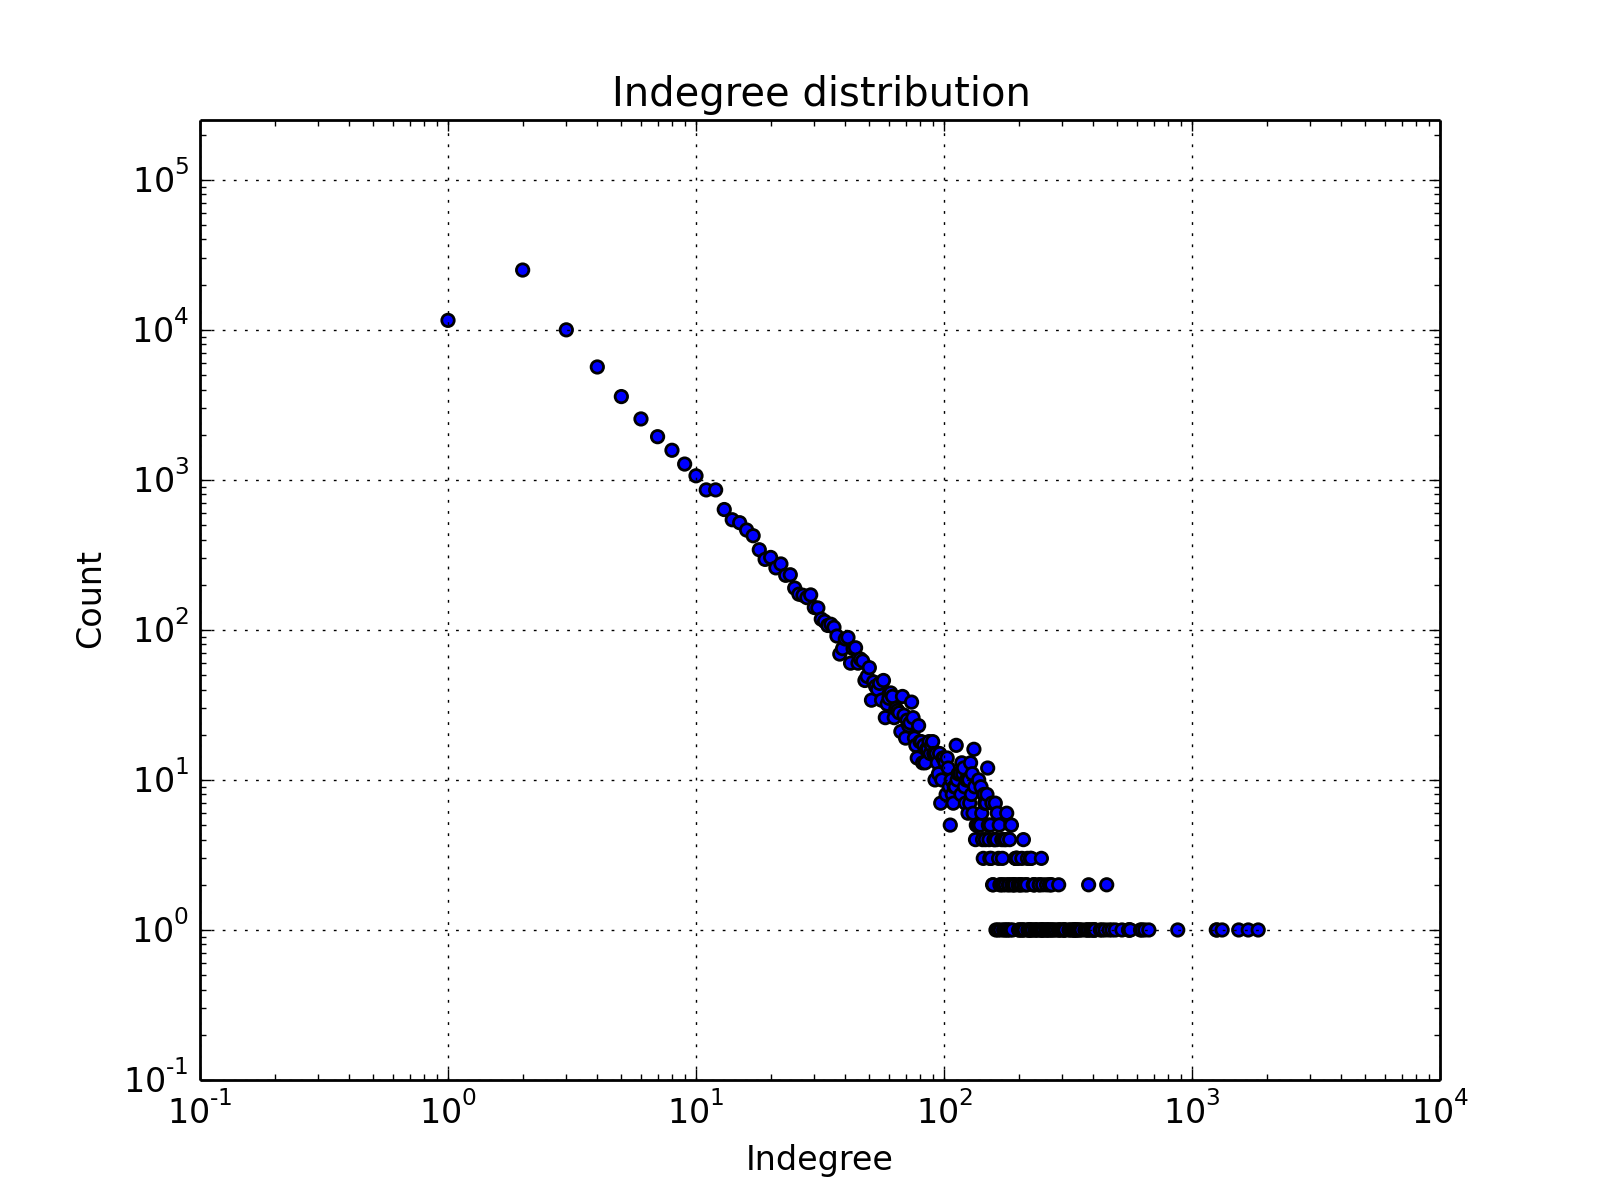
\includegraphics[width=0.35\textwidth]{FIG/IndegreeDistoutput_soc-Slashdot0811-75000.png} 
\end{tabular}
\caption{Indegree distribution plots of 6 directed graphs}
\label{fig:results}
\end{center}
\end{figure}

\begin{figure}[H]
\begin{center}
\begin{tabular}{ccc}
     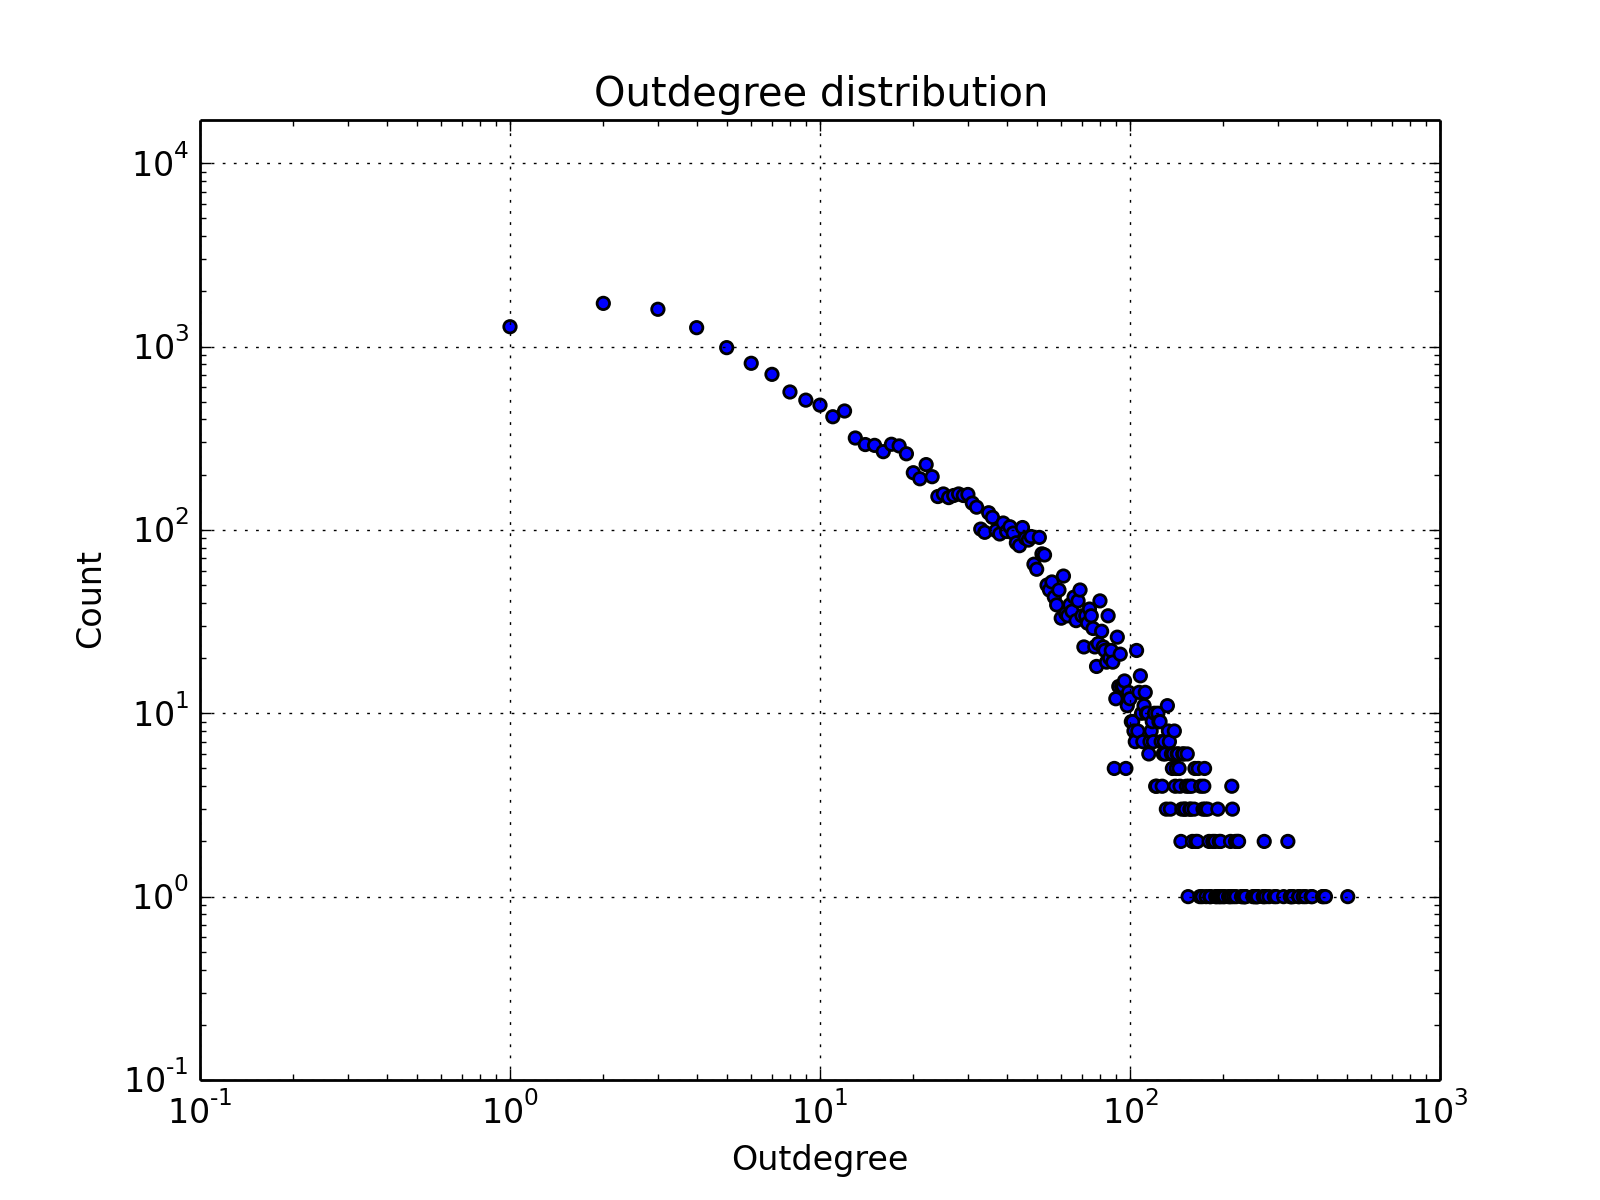
\includegraphics[width=0.35\textwidth]{FIG/OutdegreeDistoutput_ca-AstroPh.png}
     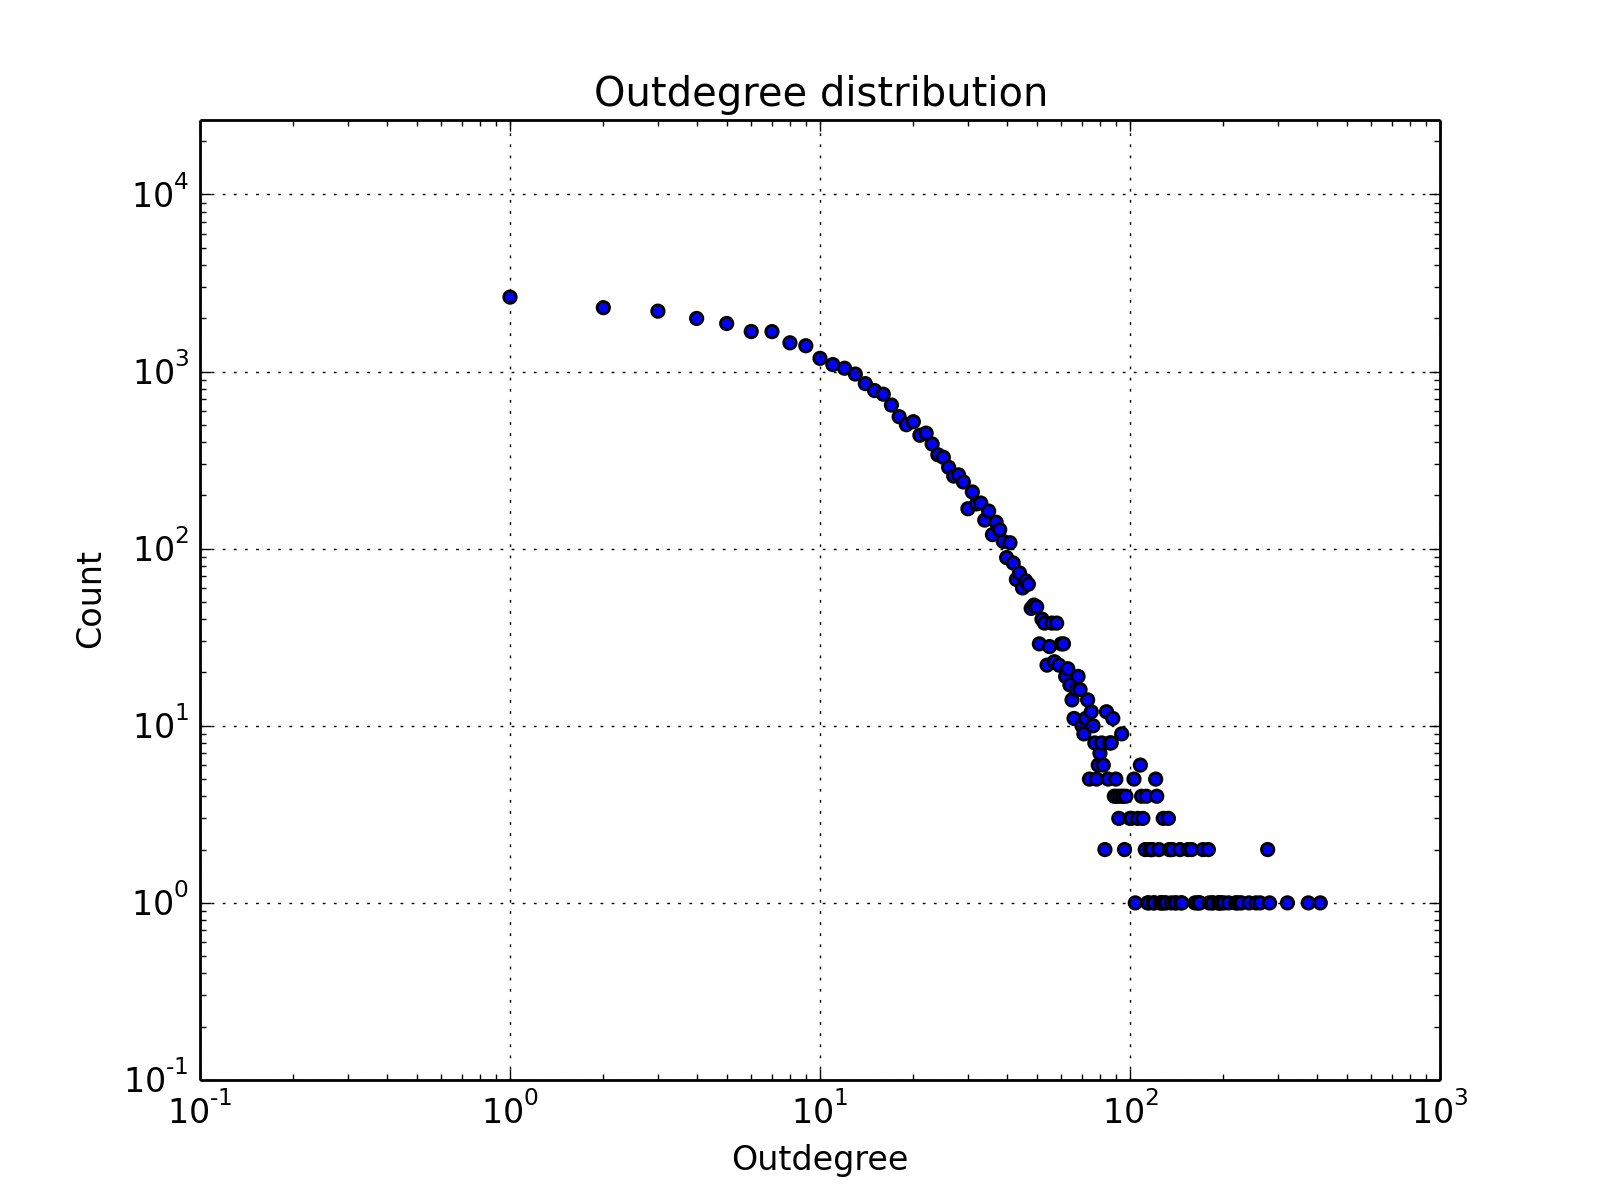
\includegraphics[width=0.35\textwidth]{FIG/OutdegreeDistoutput_cit-HepPh.png} 
     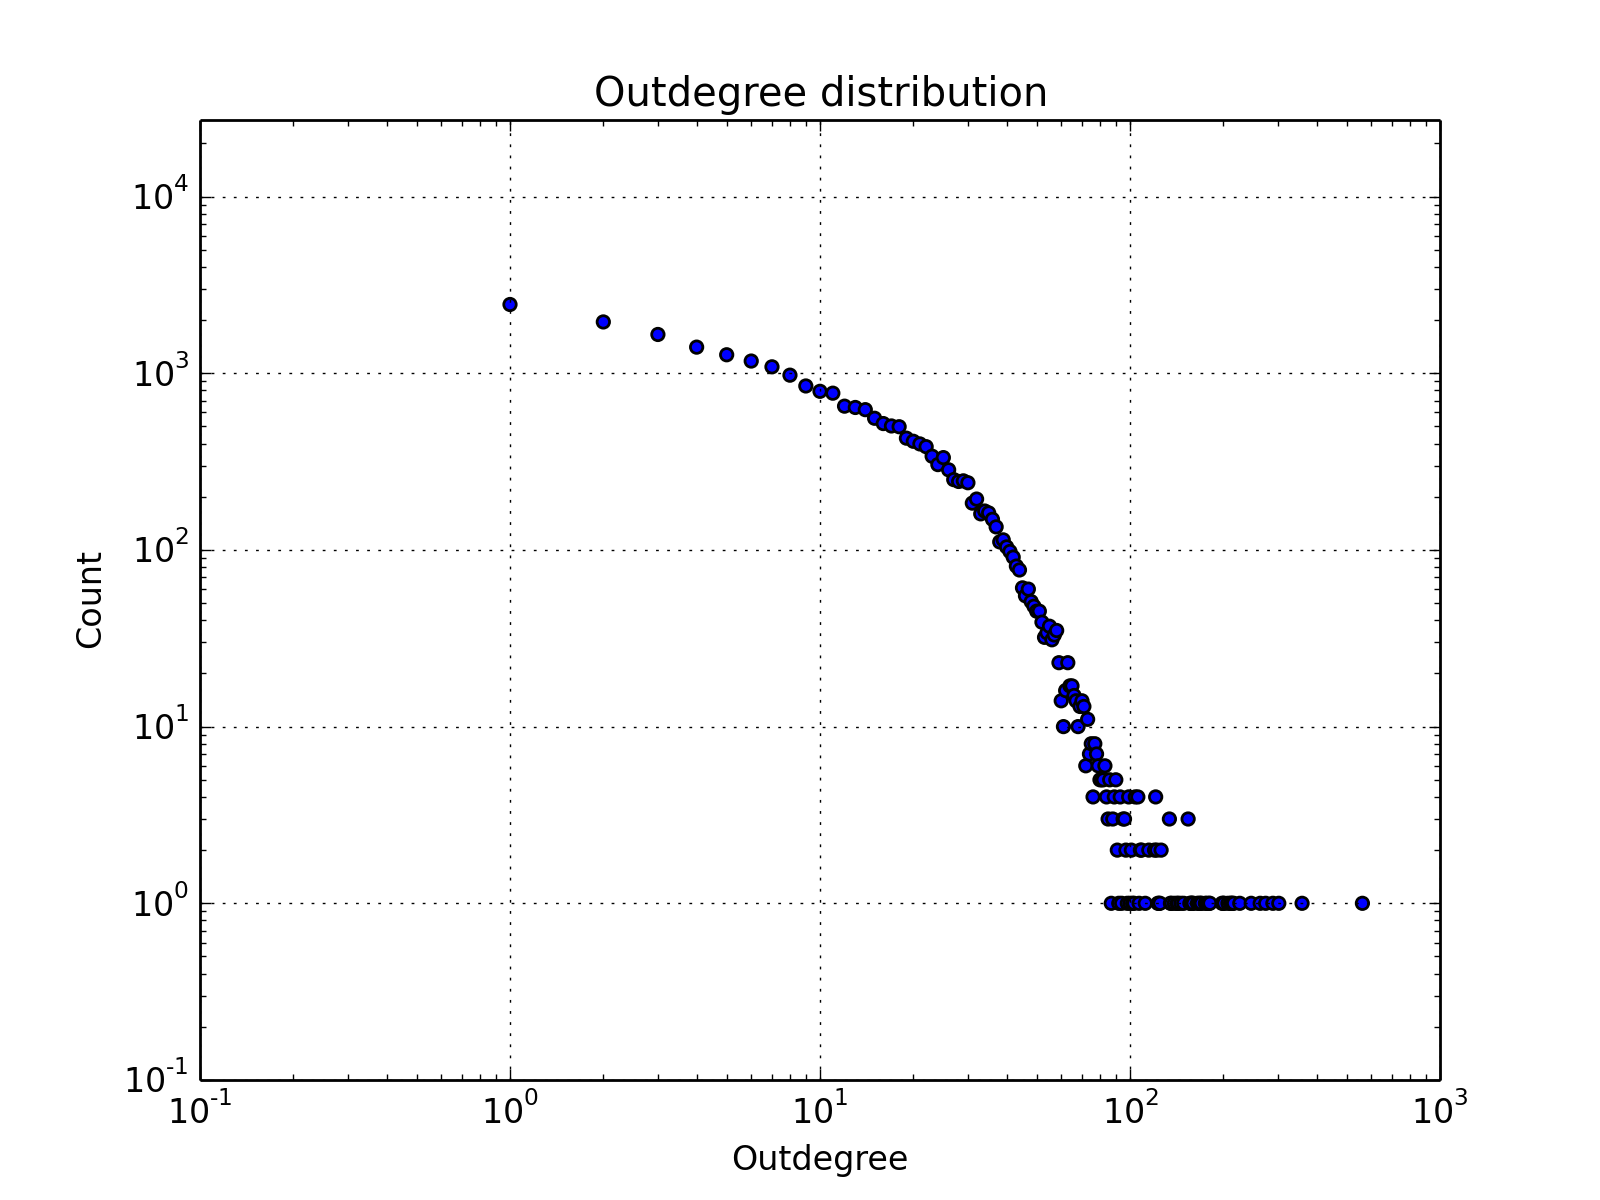
\includegraphics[width=0.35\textwidth]{FIG/OutdegreeDistoutput_cit-HepTh.png} \\
     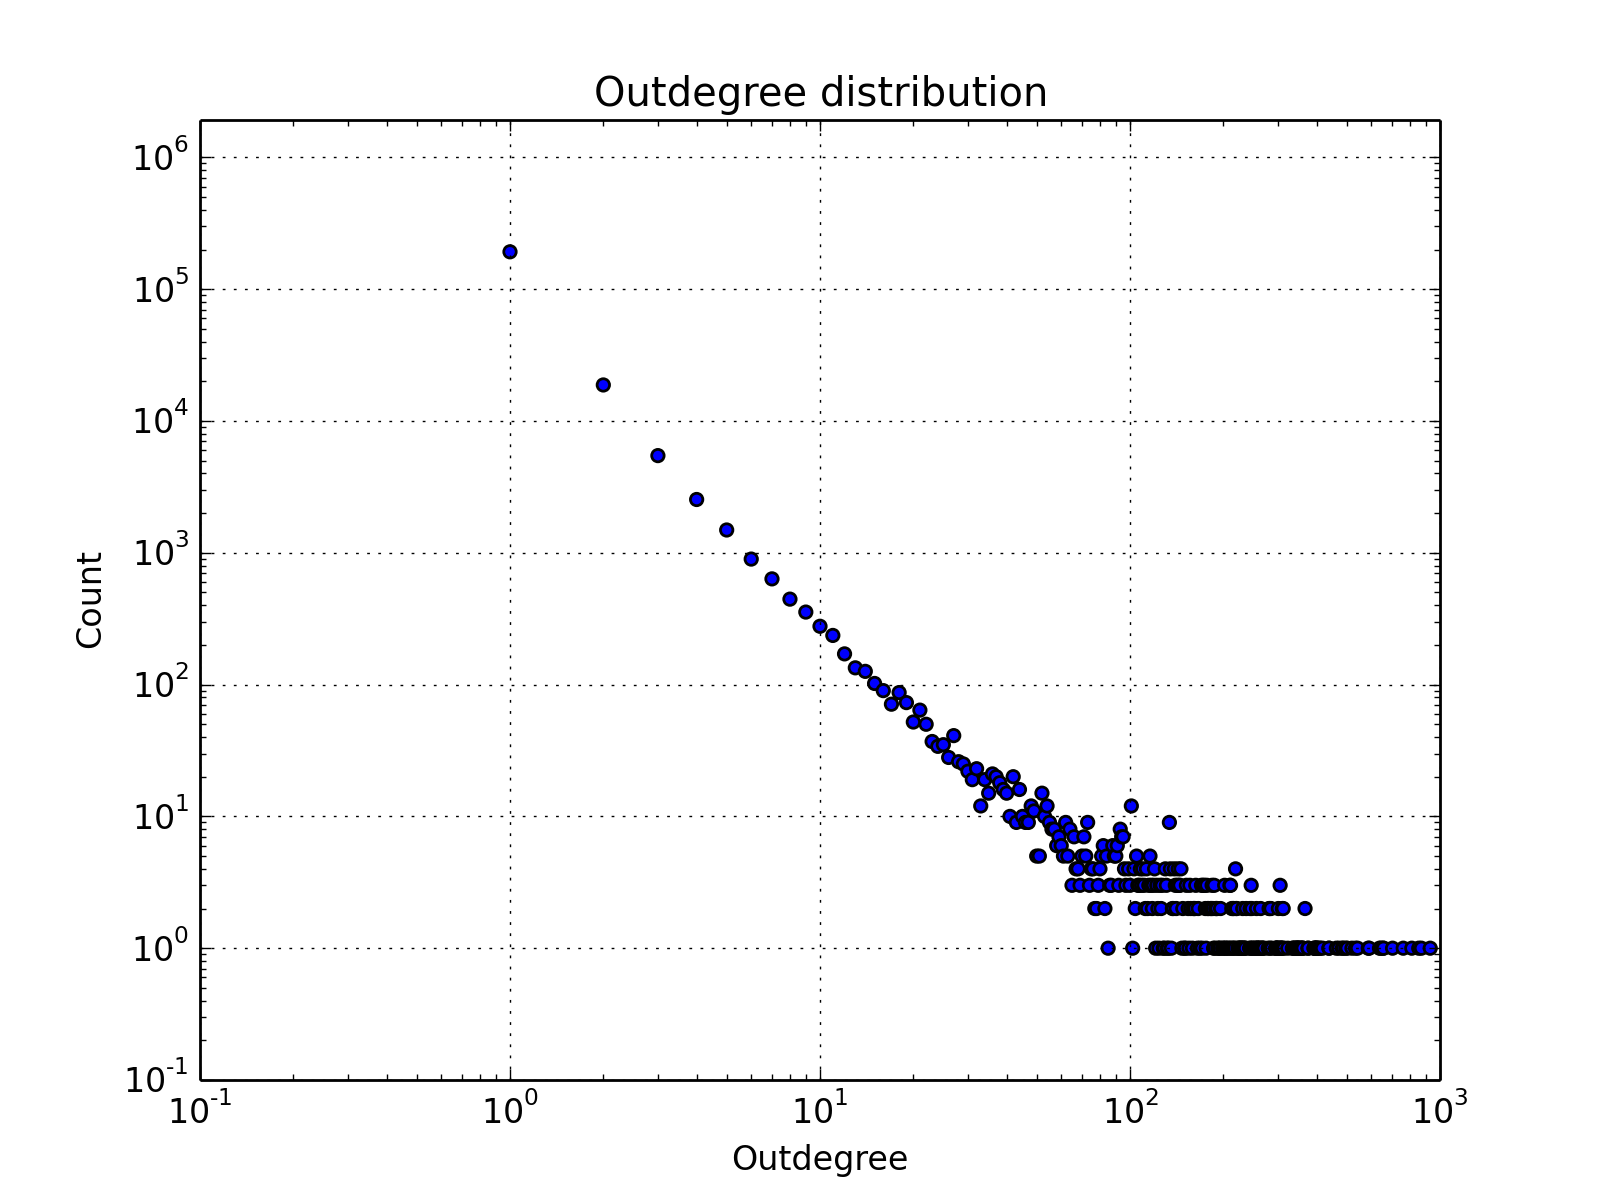
\includegraphics[width=0.35\textwidth]{FIG/OutdegreeDistoutput_email-EuAll.png} 
     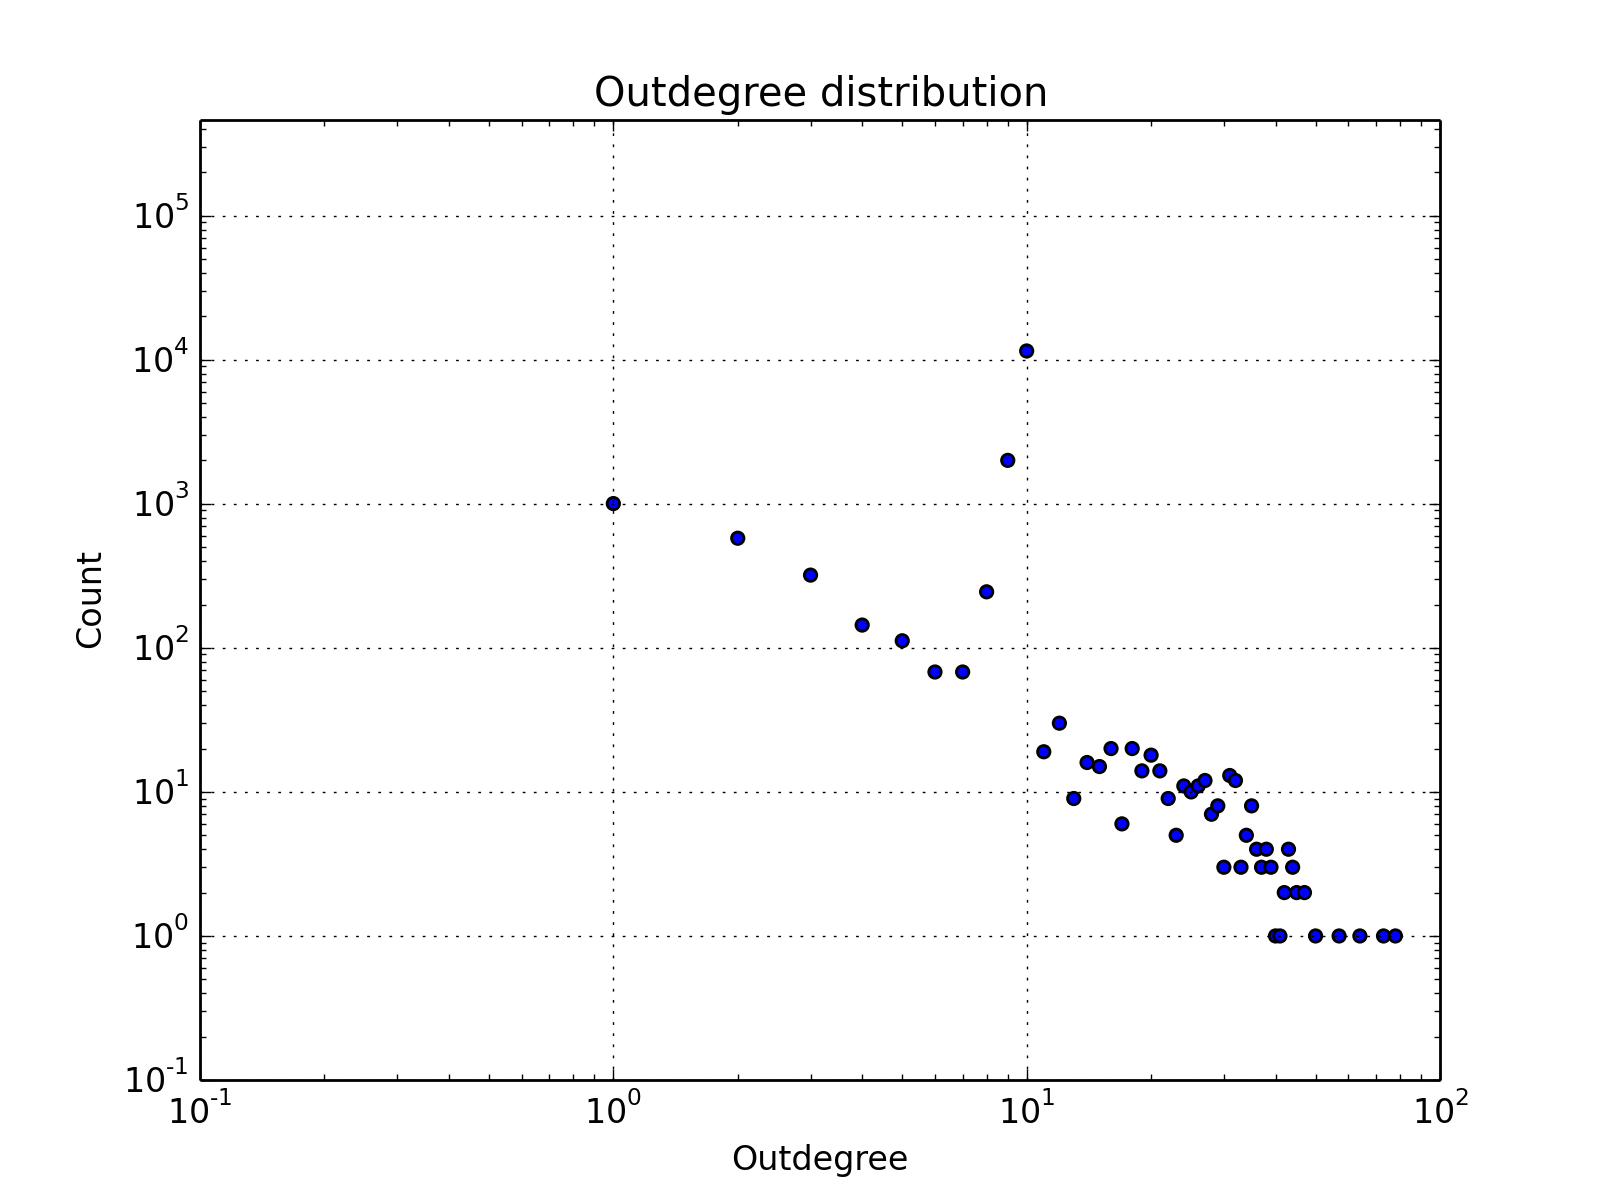
\includegraphics[width=0.35\textwidth]{FIG/OutdegreeDistoutput_p2p-Gnutella31.png} 
     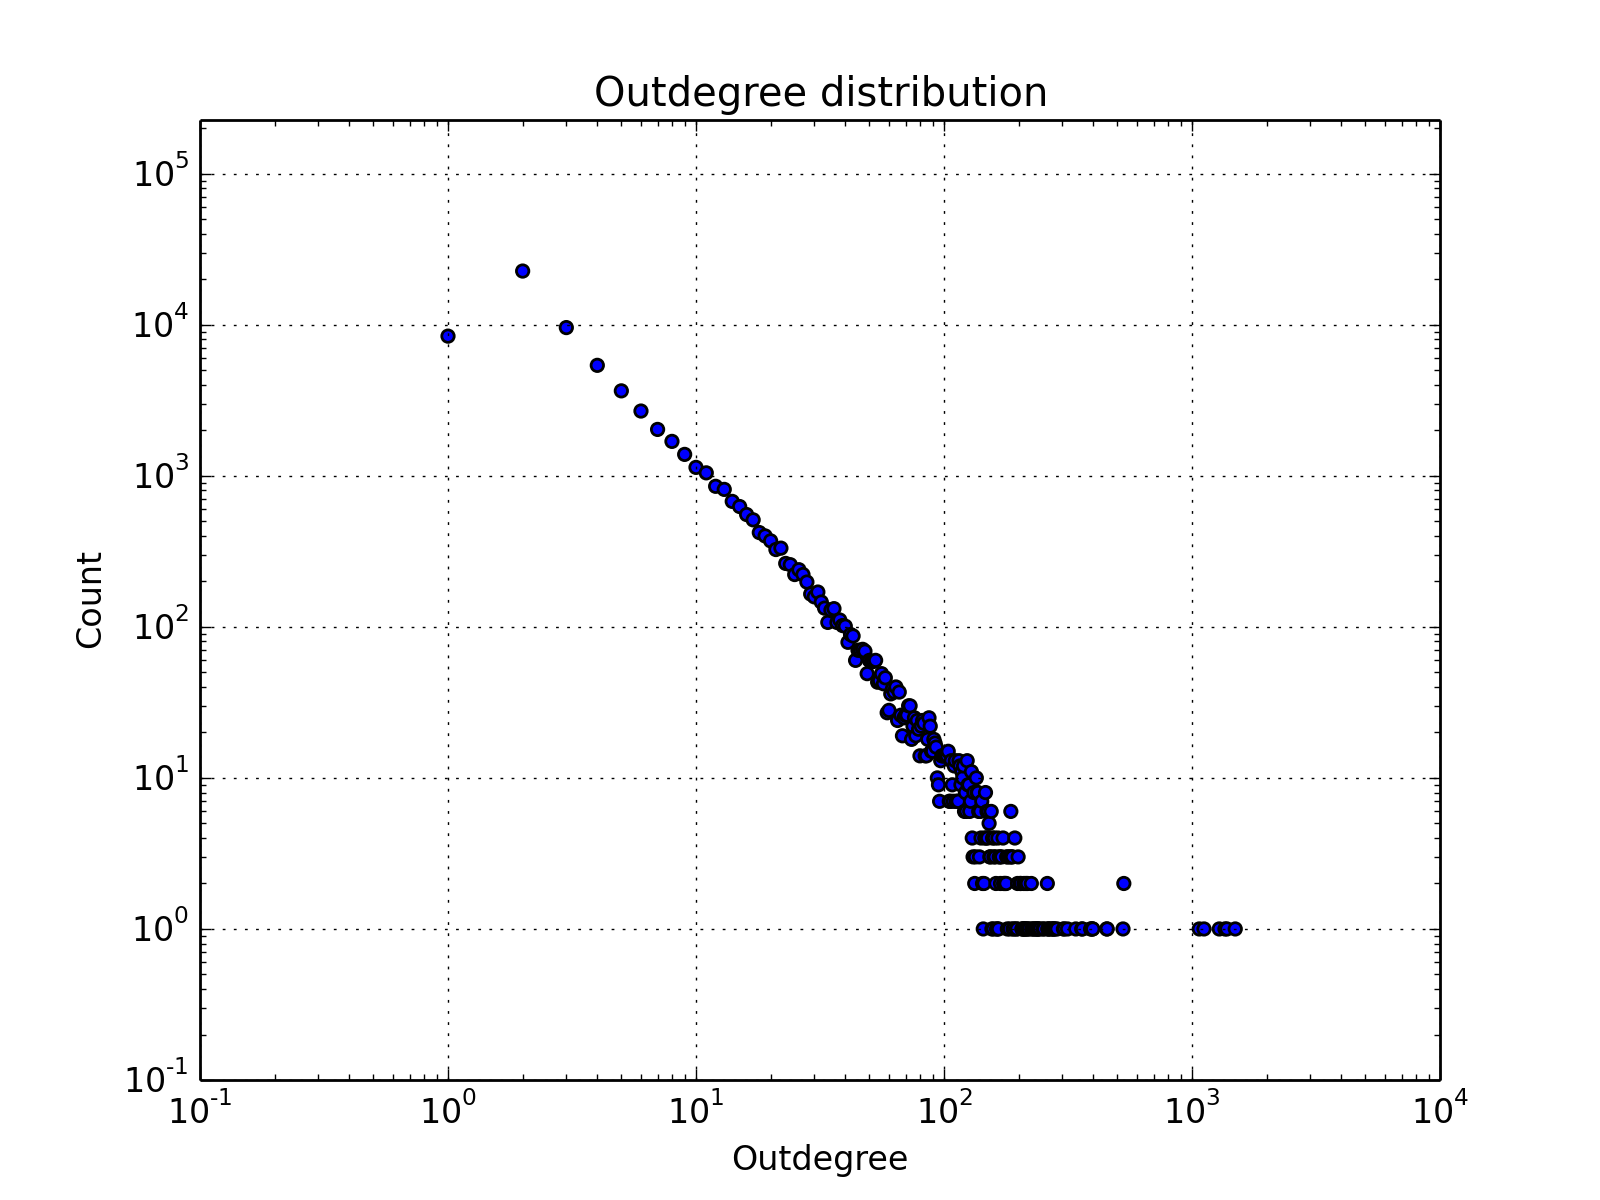
\includegraphics[width=0.35\textwidth]{FIG/OutdegreeDistoutput_soc-Slashdot0811-75000.png} 
\end{tabular}
\caption{Outdegree distribution plots of 6 directed graphs}
\label{fig:results}
\end{center}
\end{figure}

\textbf{Observation:}
\par Most graphs obey the power law, most nodes have small degree, only few nodes have high degree. In log-log space as shown above, we can draw a line to fit the scatter points.

\subsection{PageRank}
We can plot Rank vs. PageRank in log space:

\begin{figure}[H]
\begin{center}
\begin{tabular}{ccc}
     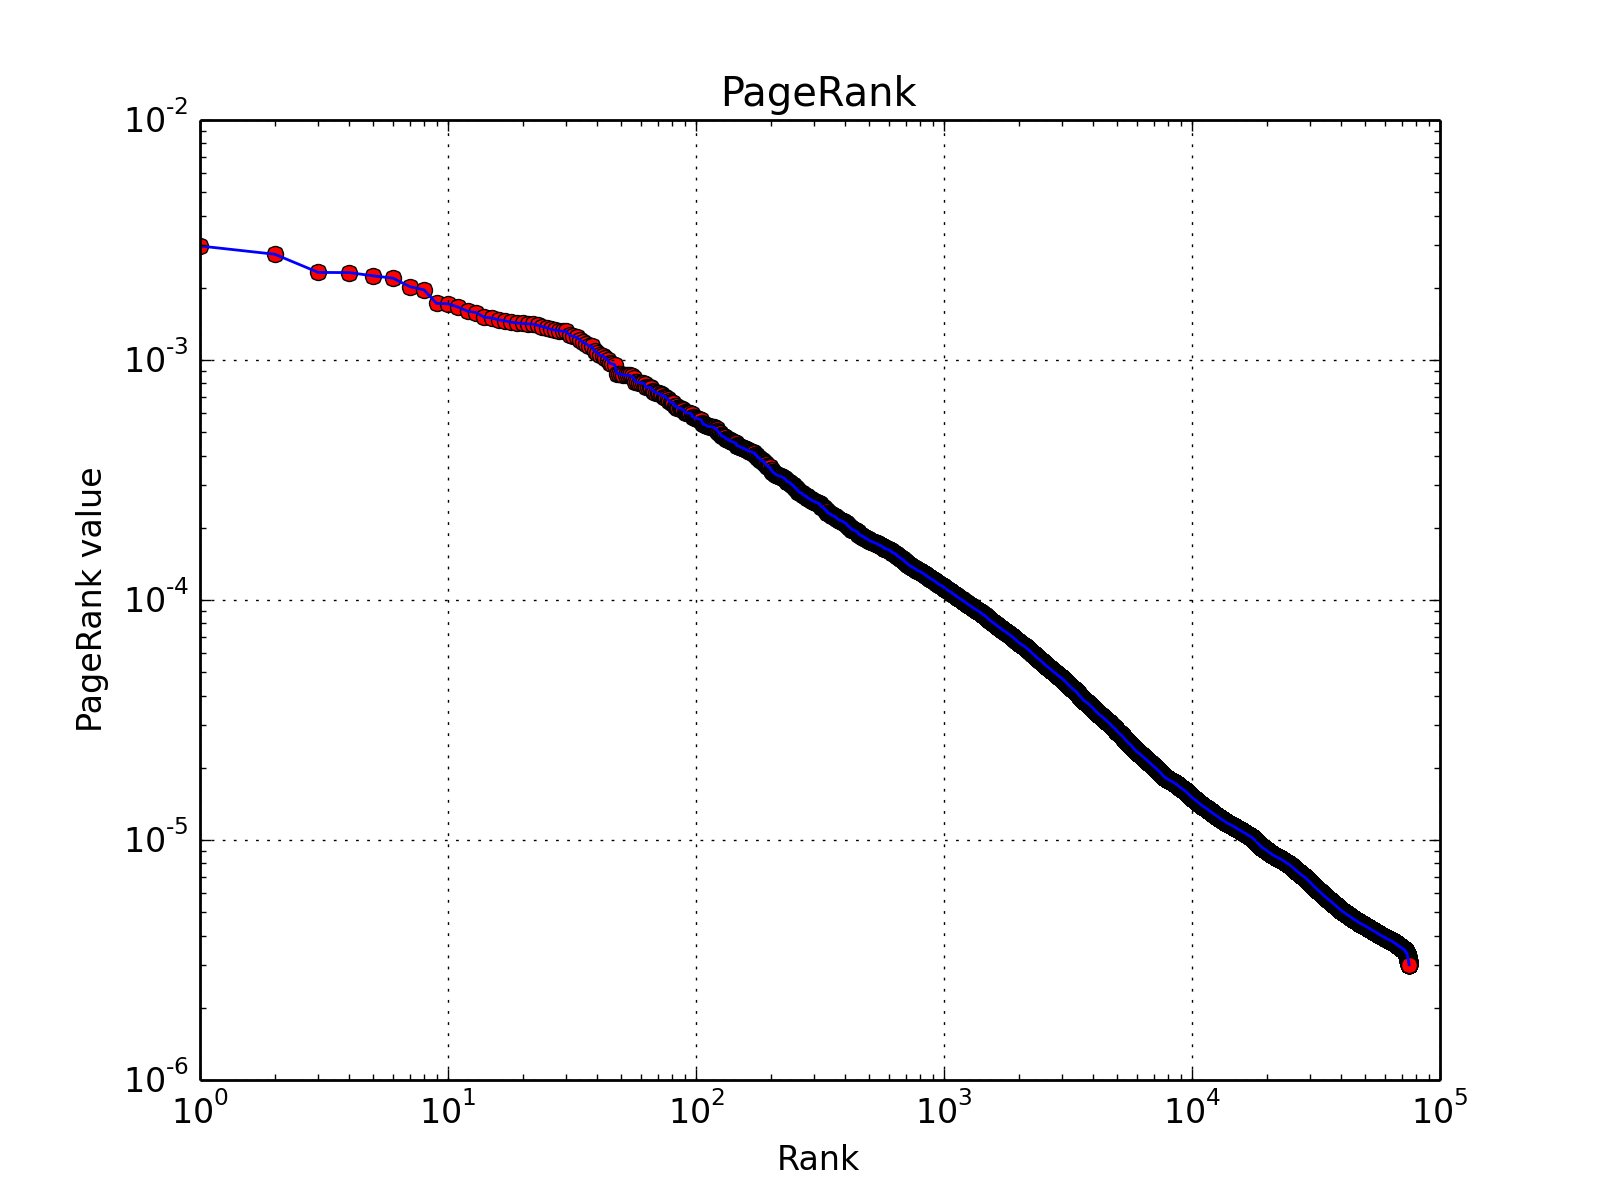
\includegraphics[width=0.35\textwidth]{FIG/pageRankoutput_as-skitter.png} 
     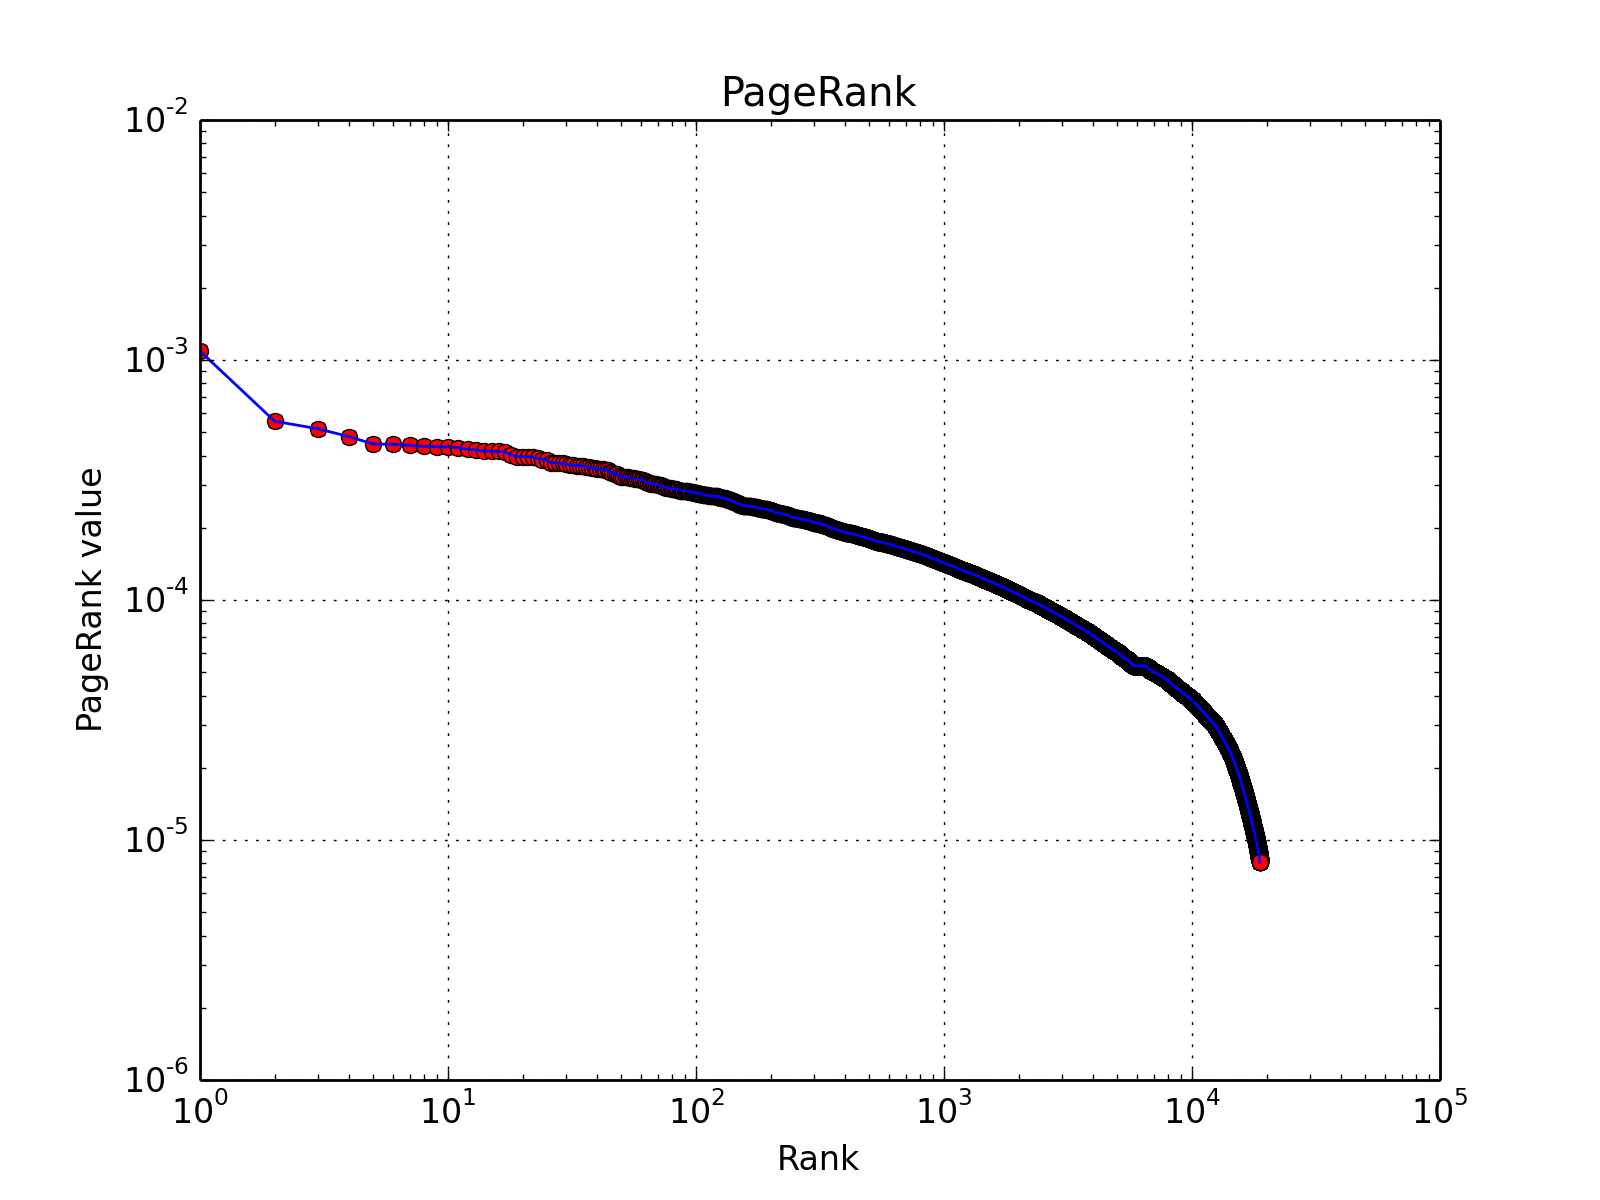
\includegraphics[width=0.35\textwidth]{FIG/pageRankoutput_ca-AstroPh.png}
     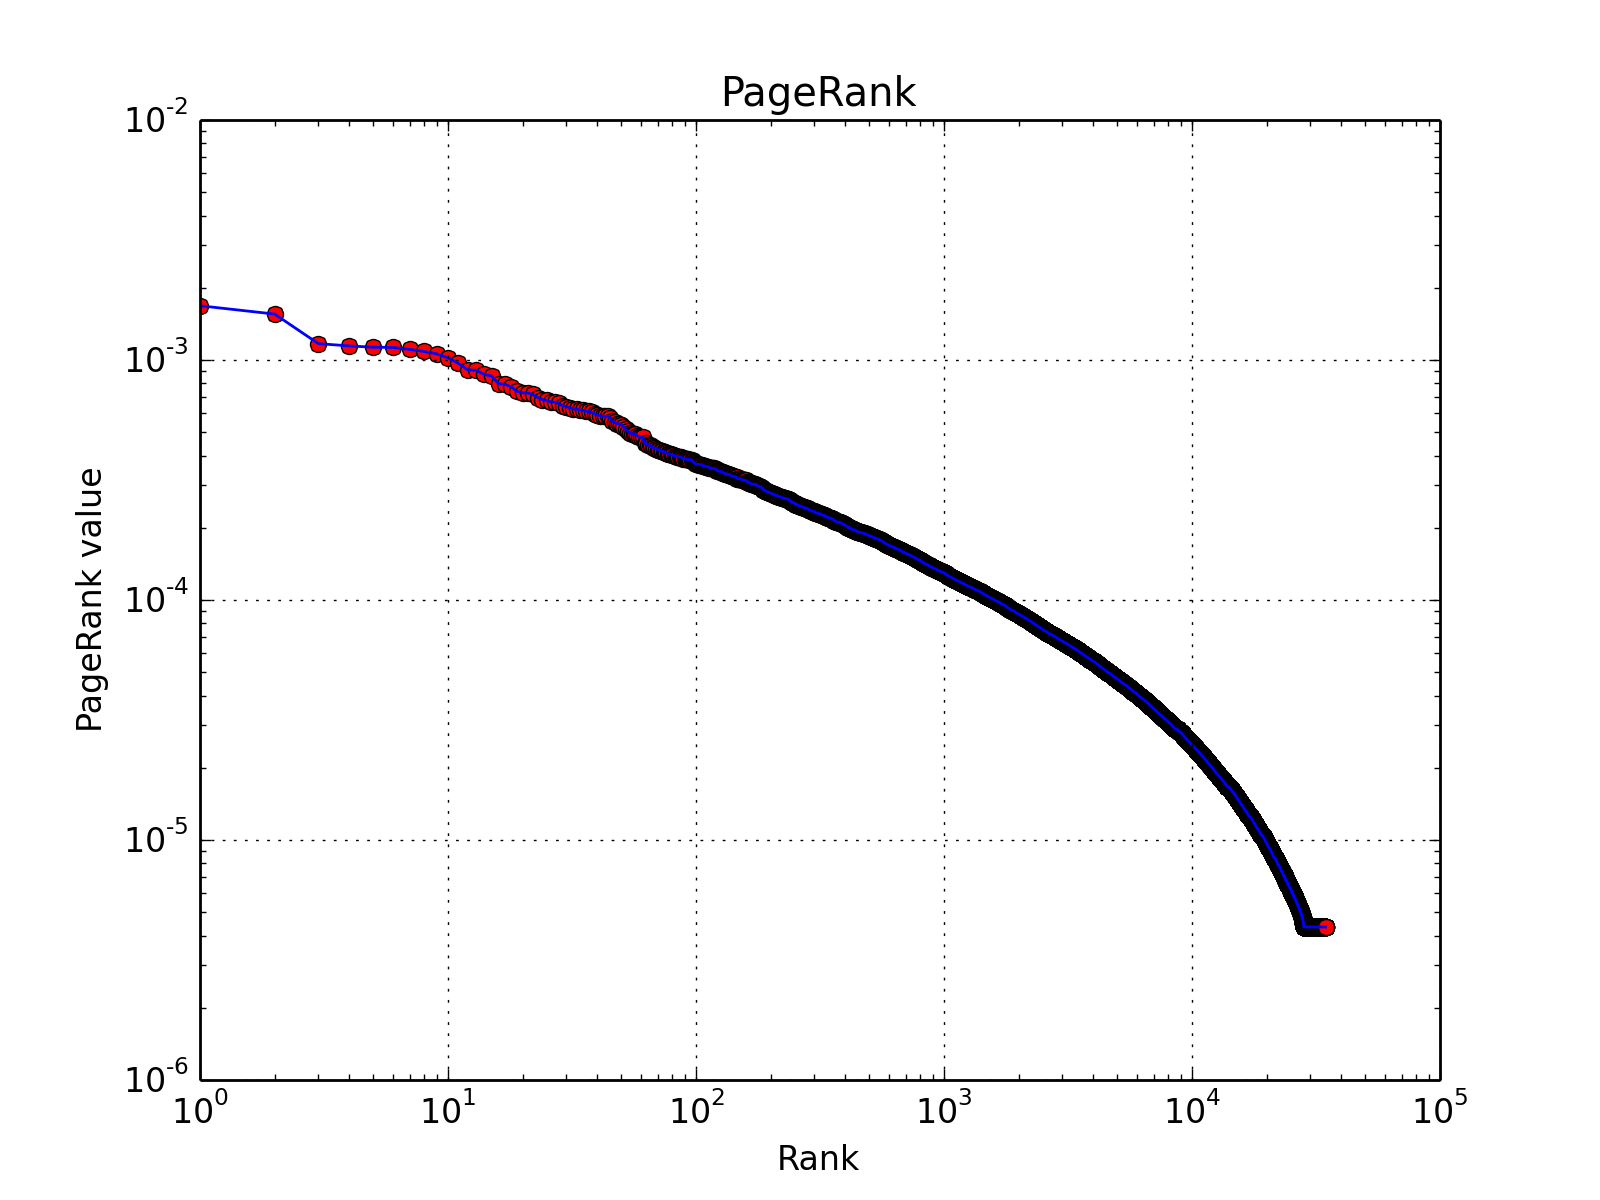
\includegraphics[width=0.35\textwidth]{FIG/pageRankoutput_cit-HepPh.png} \\
     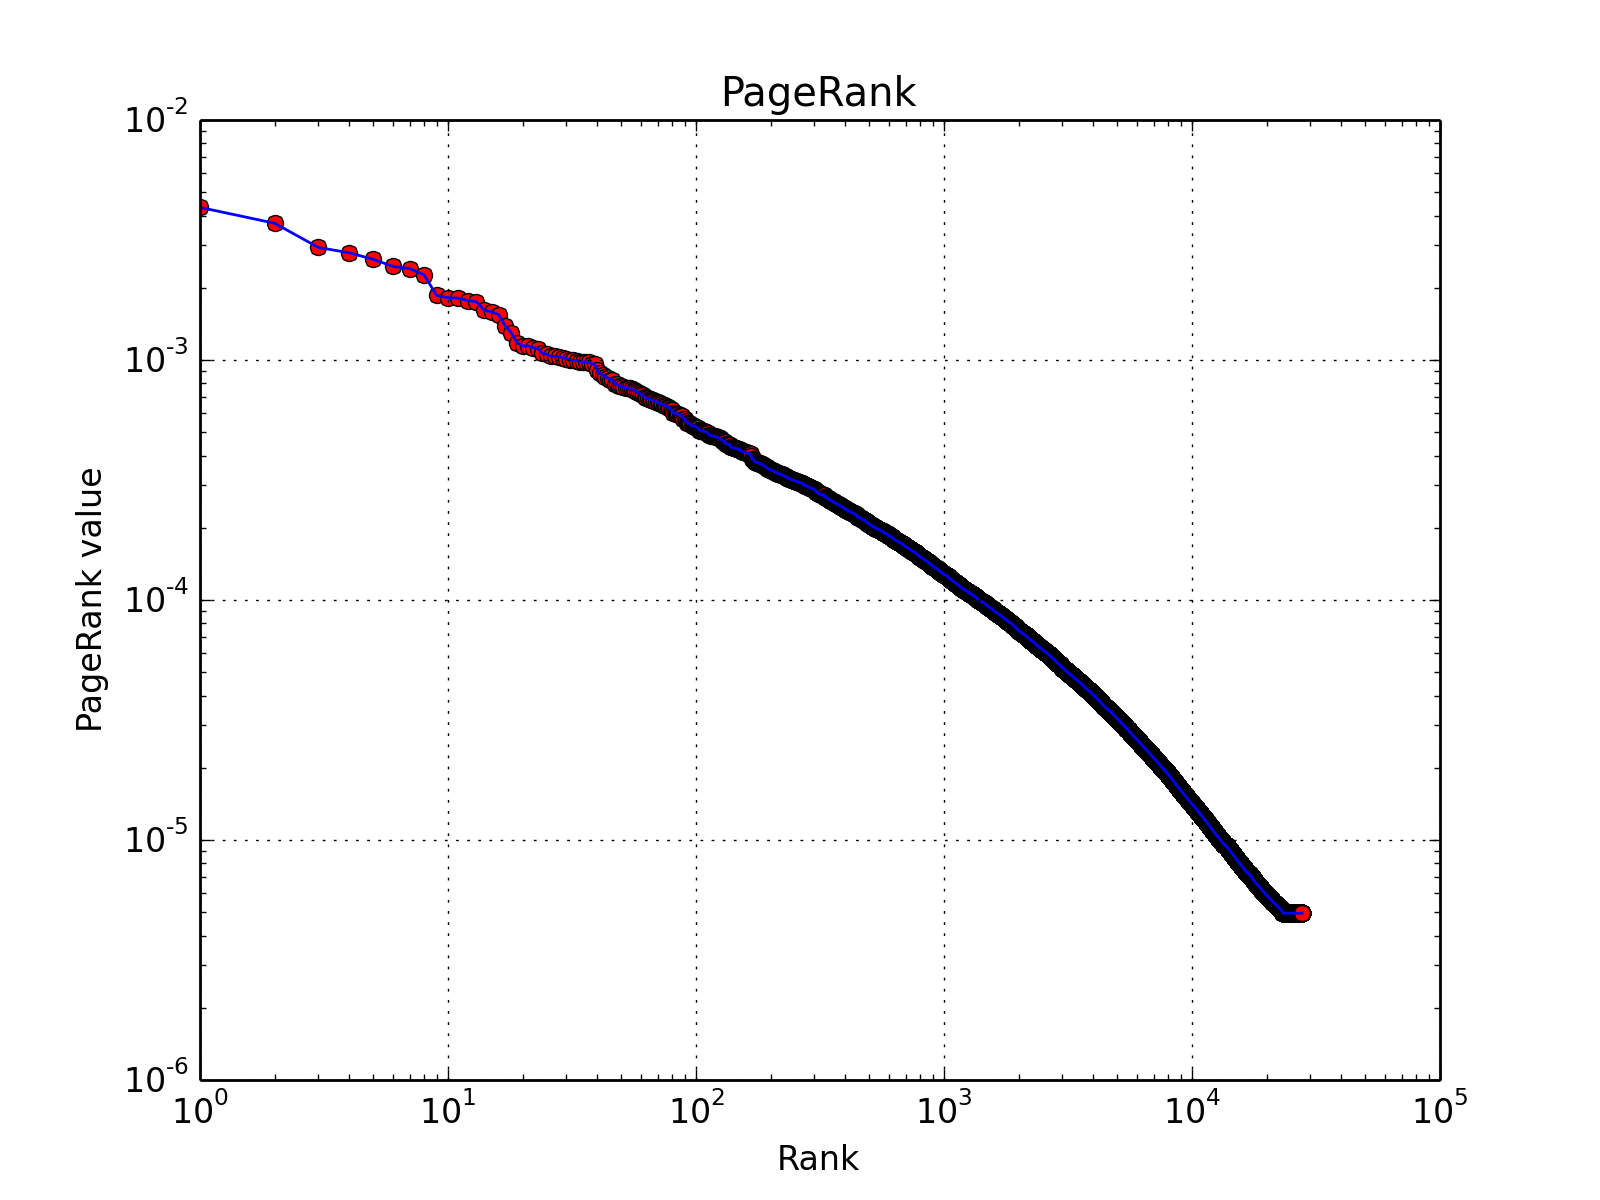
\includegraphics[width=0.35\textwidth]{FIG/pageRankoutput_cit-HepTh.png} 
     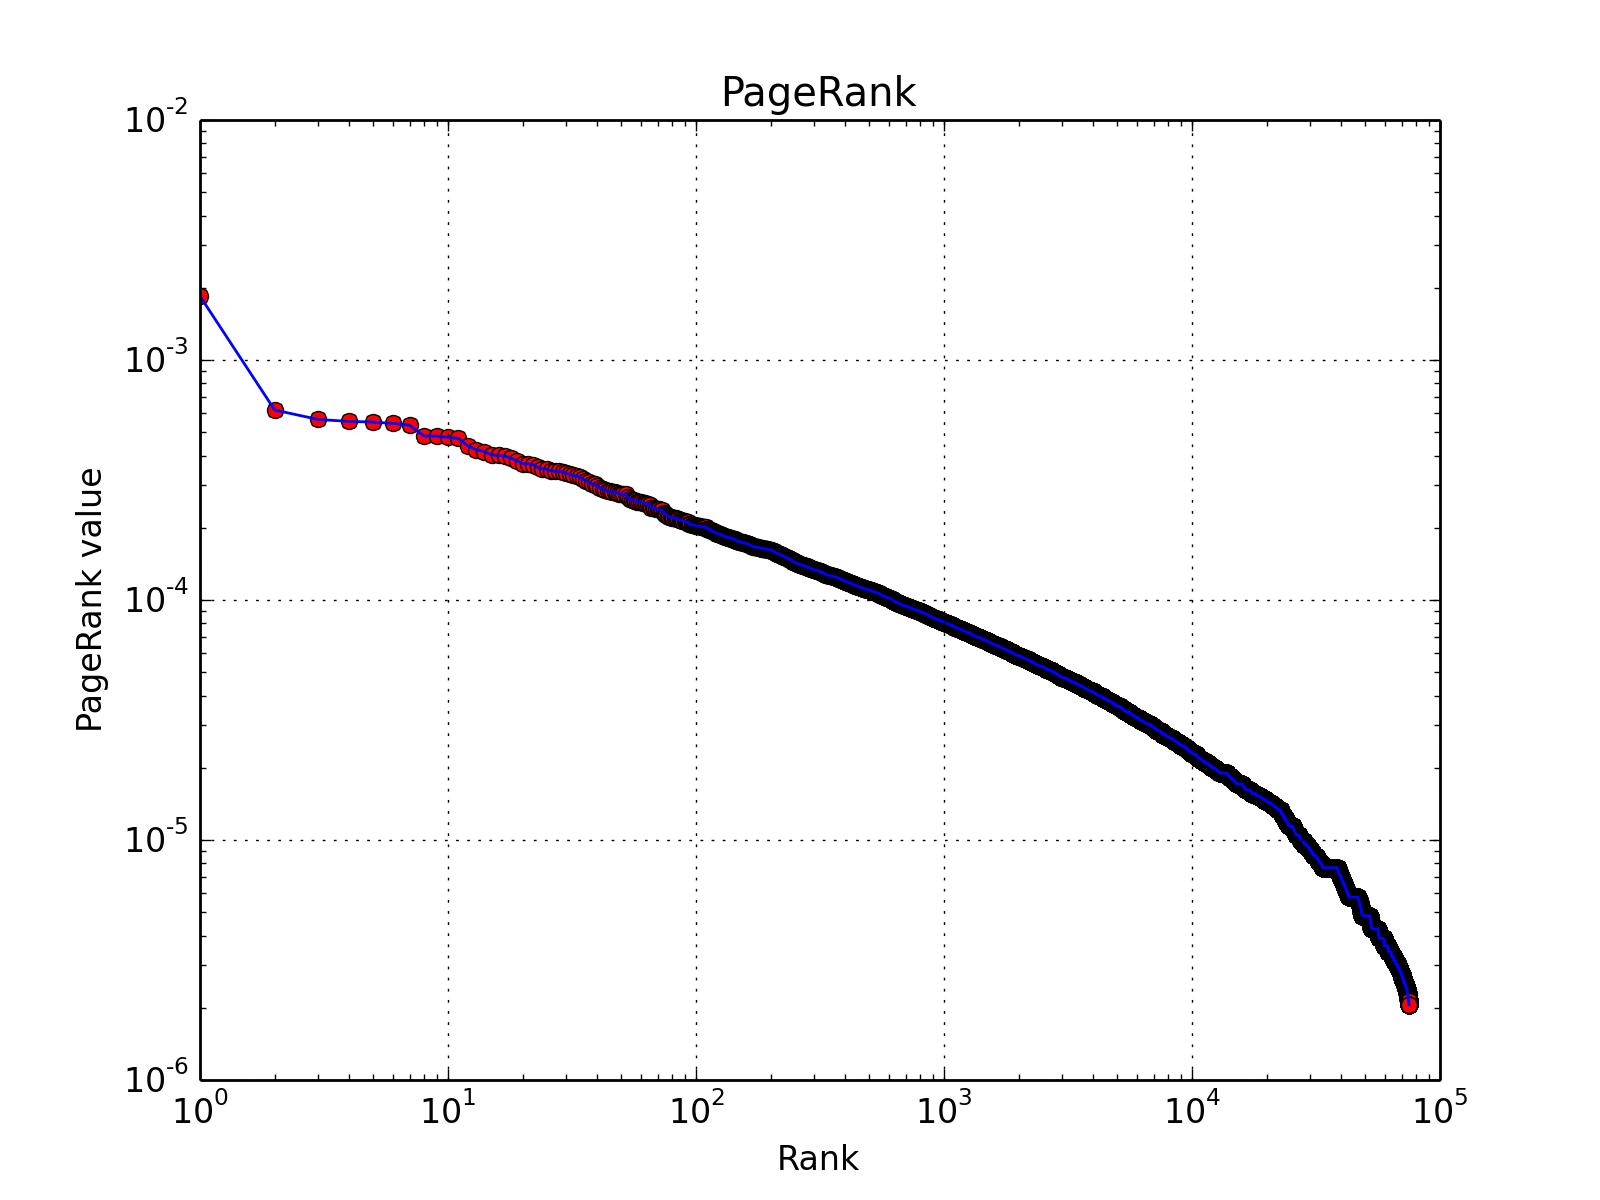
\includegraphics[width=0.35\textwidth]{FIG/pageRankoutput_com-amazon.png} 
     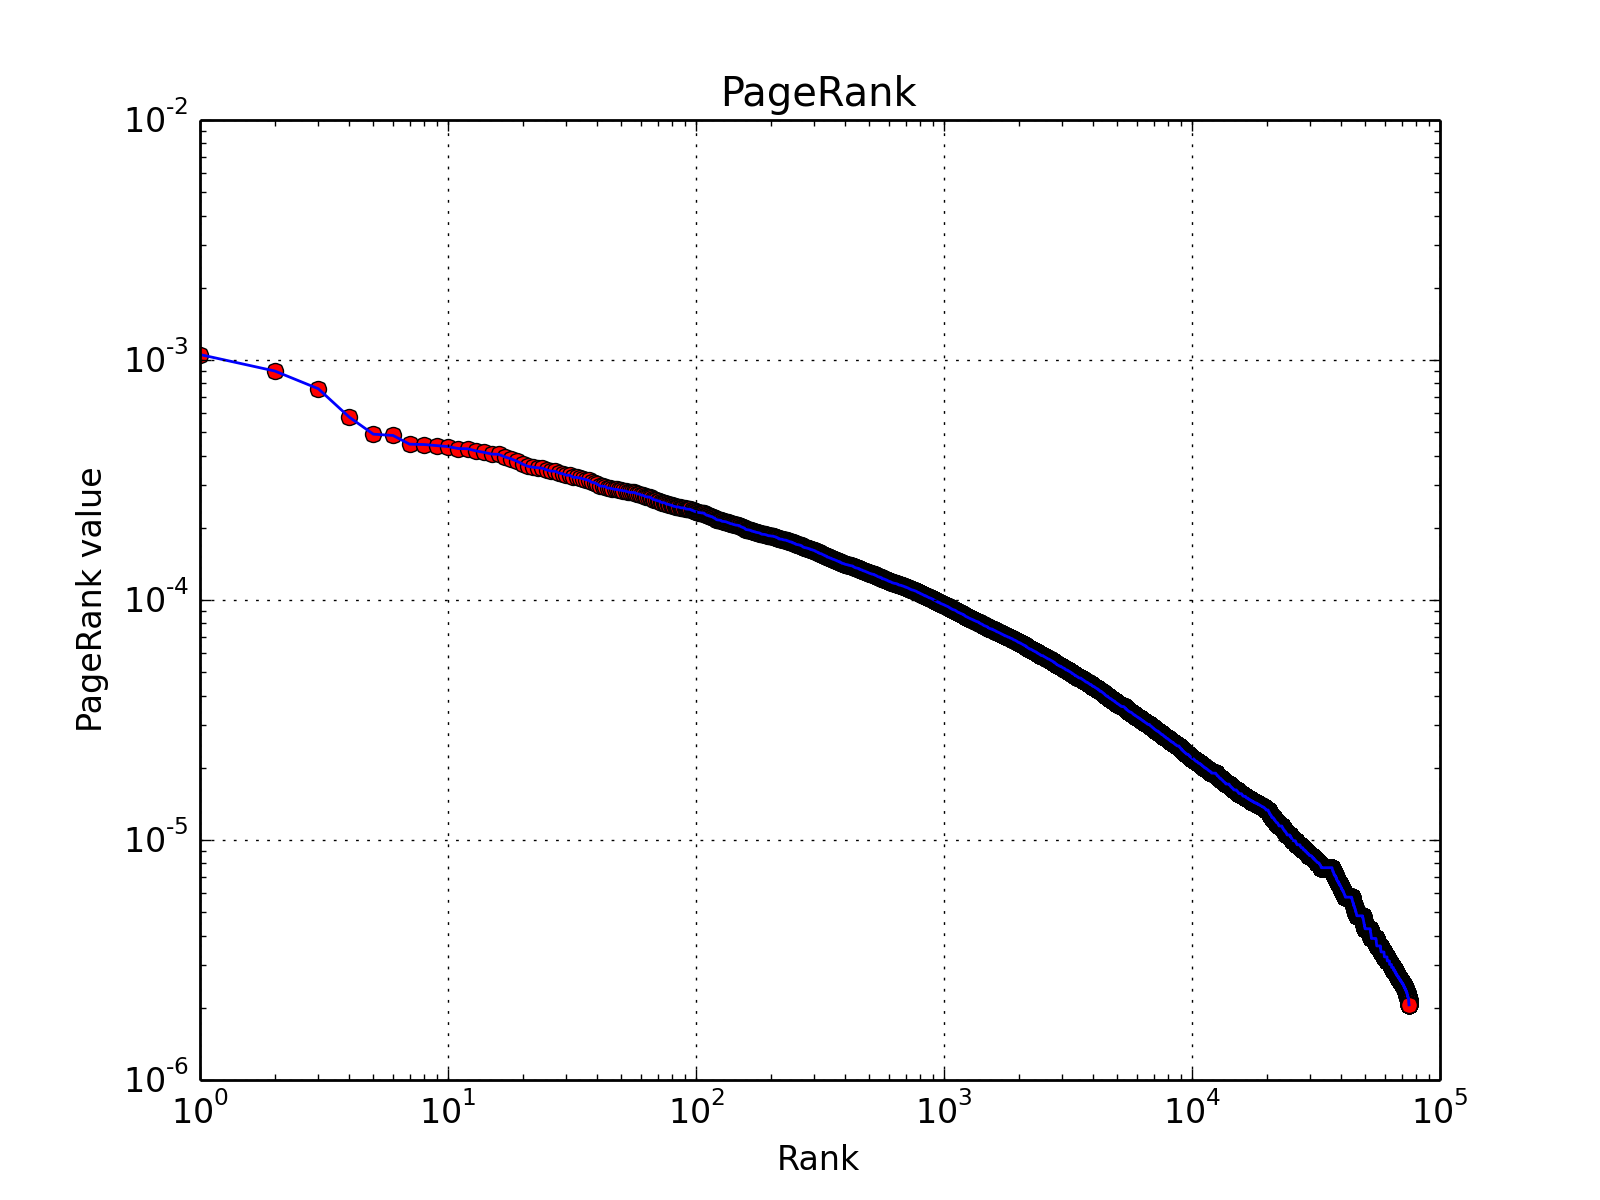
\includegraphics[width=0.35\textwidth]{FIG/pageRankoutput_com-dblp.png} \\
     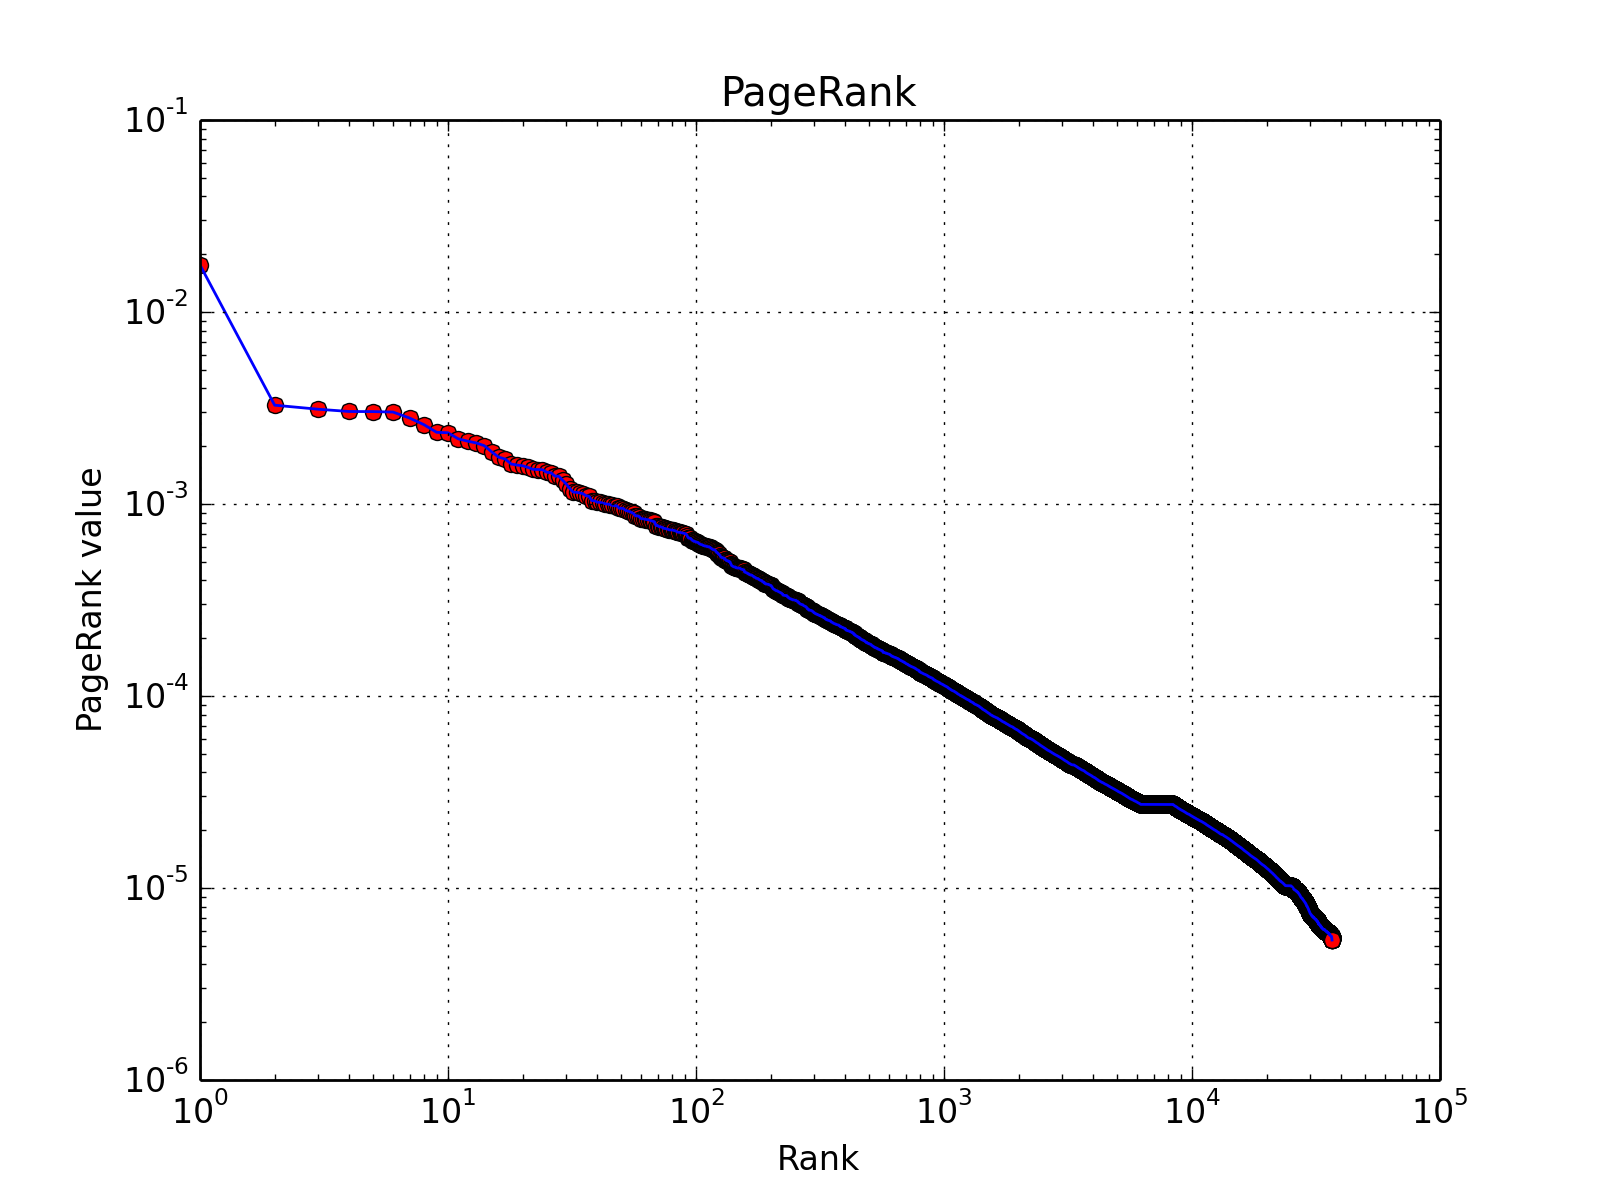
\includegraphics[width=0.35\textwidth]{FIG/pageRankoutput_email-Enron.png} 
     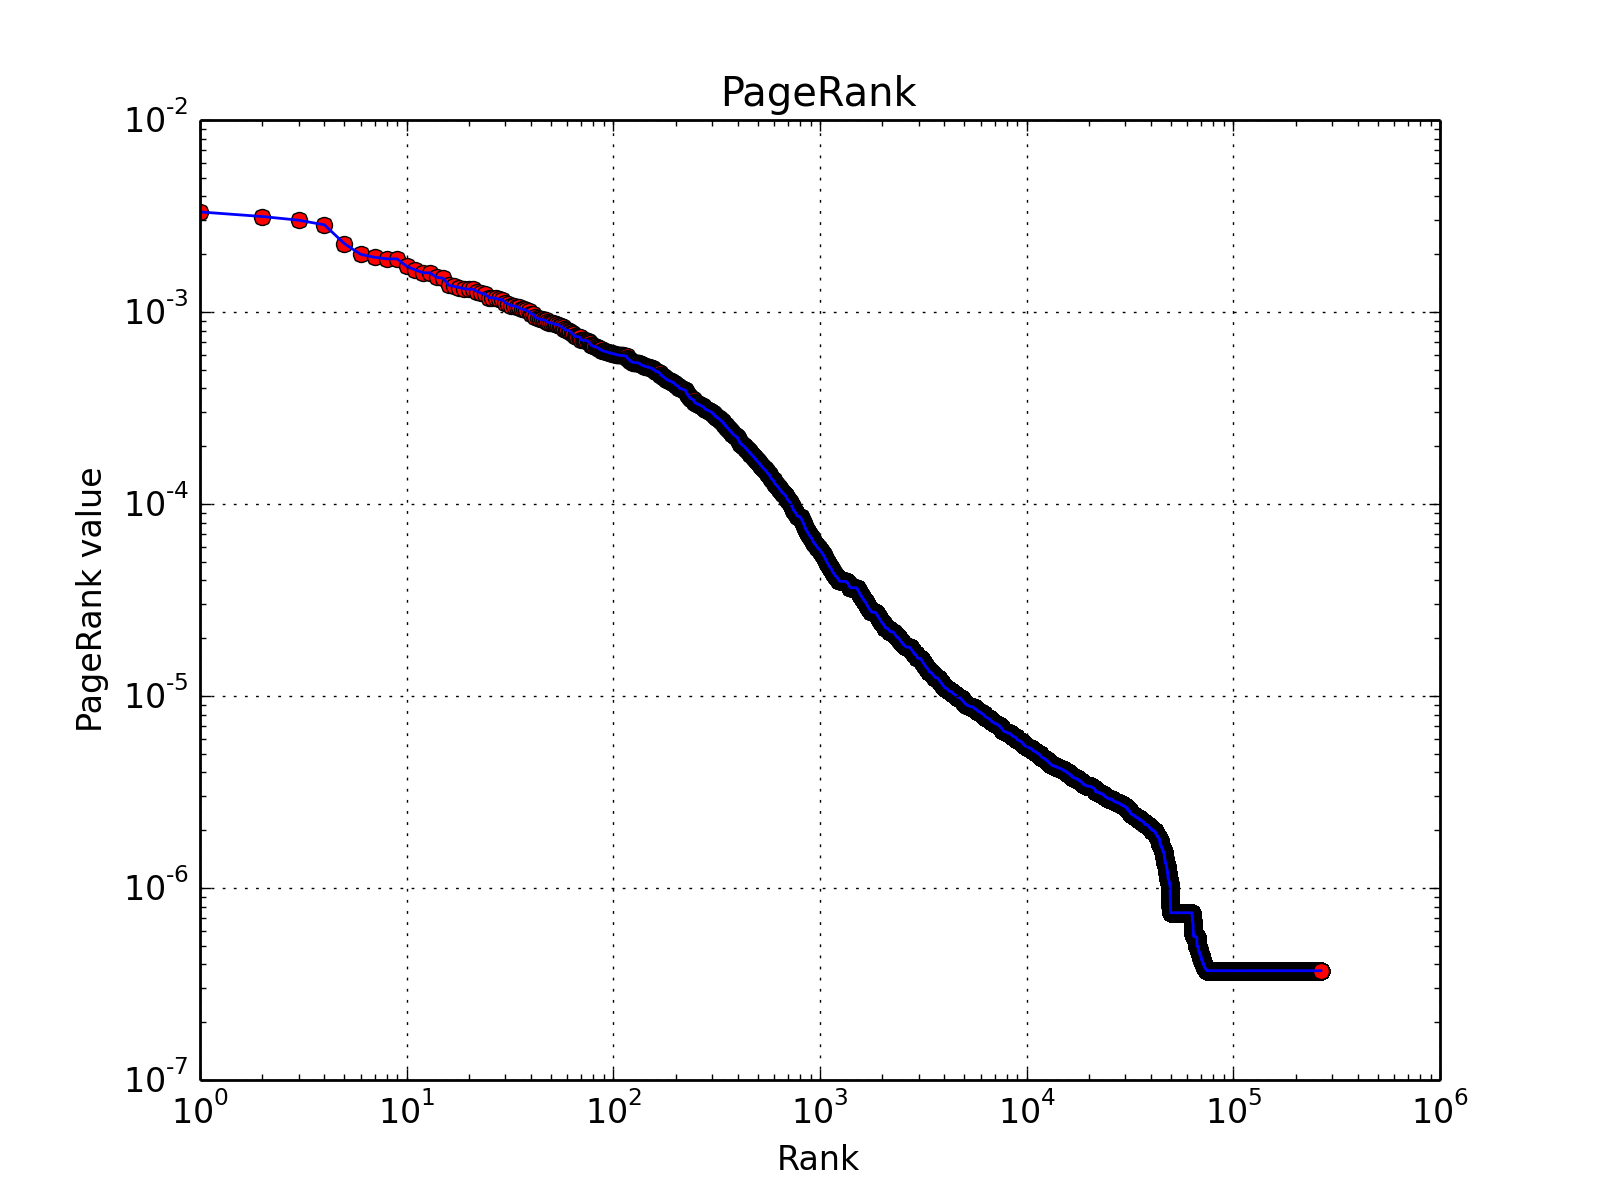
\includegraphics[width=0.35\textwidth]{FIG/pageRankoutput_email-EuAll.png} 
     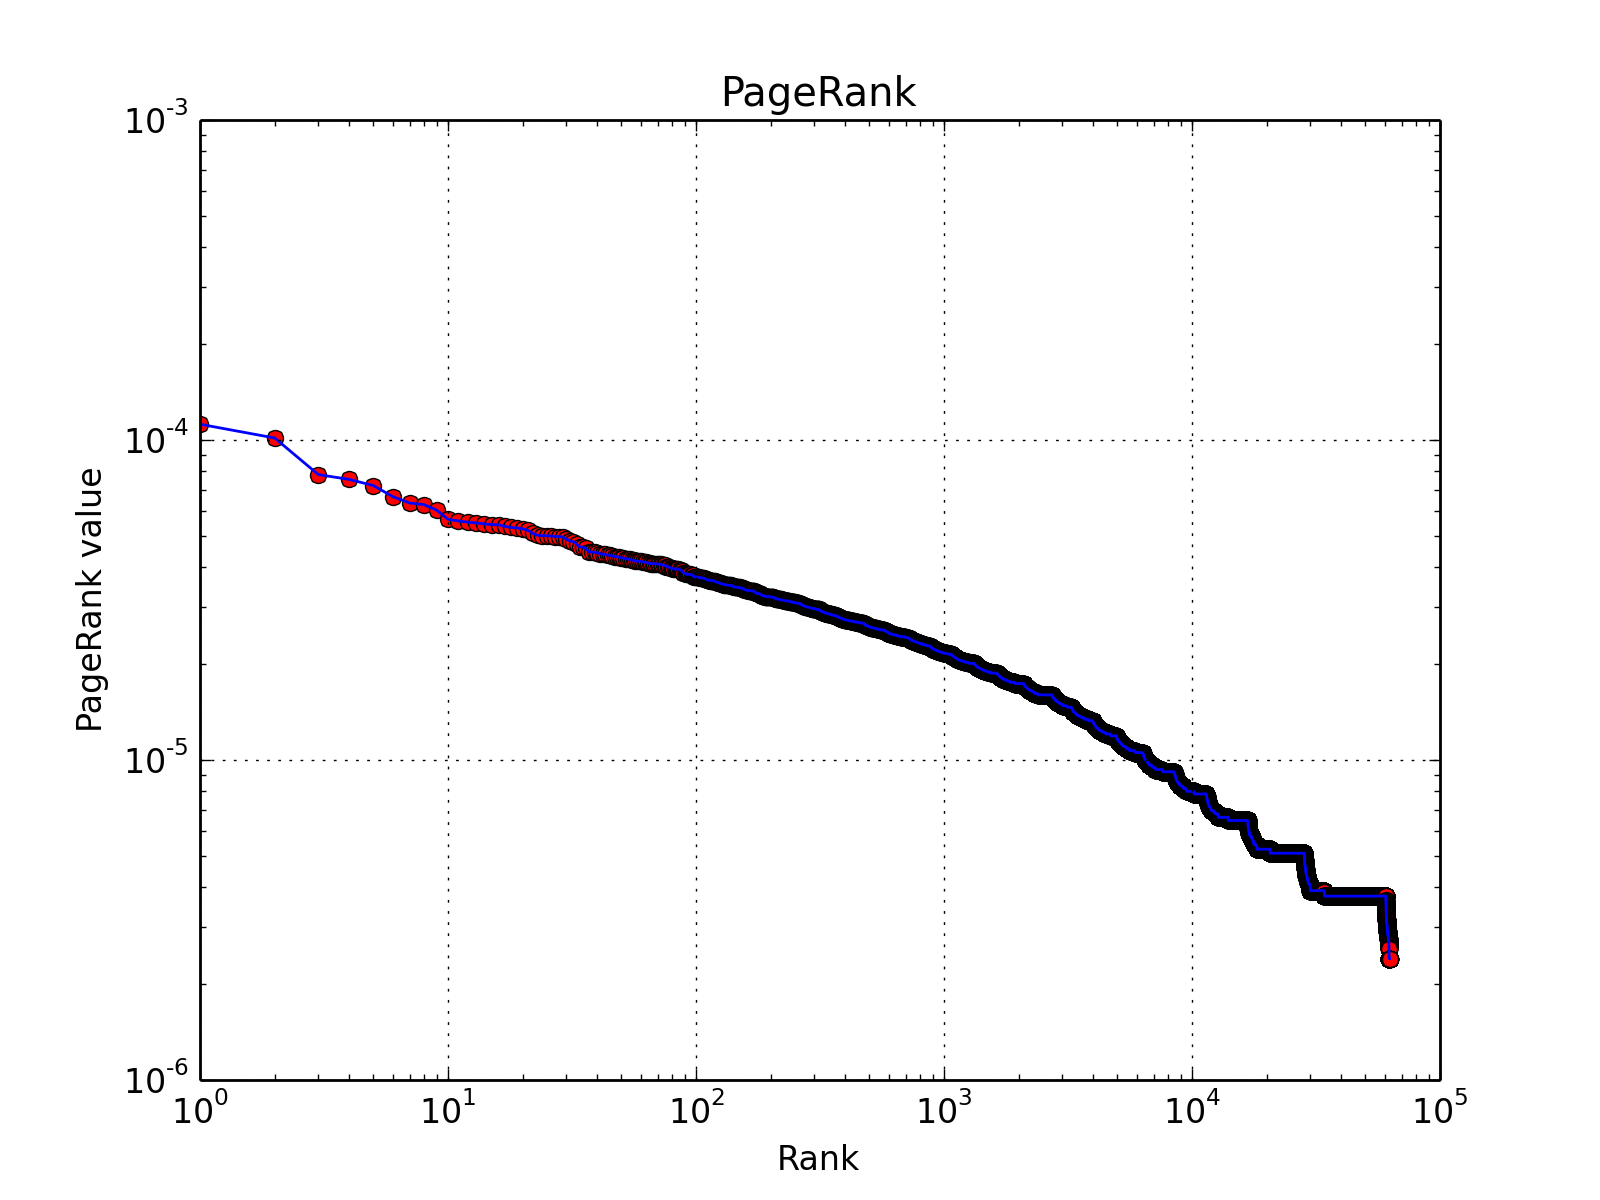
\includegraphics[width=0.35\textwidth]{FIG/pageRankoutput_p2p-Gnutella31.png} \\
     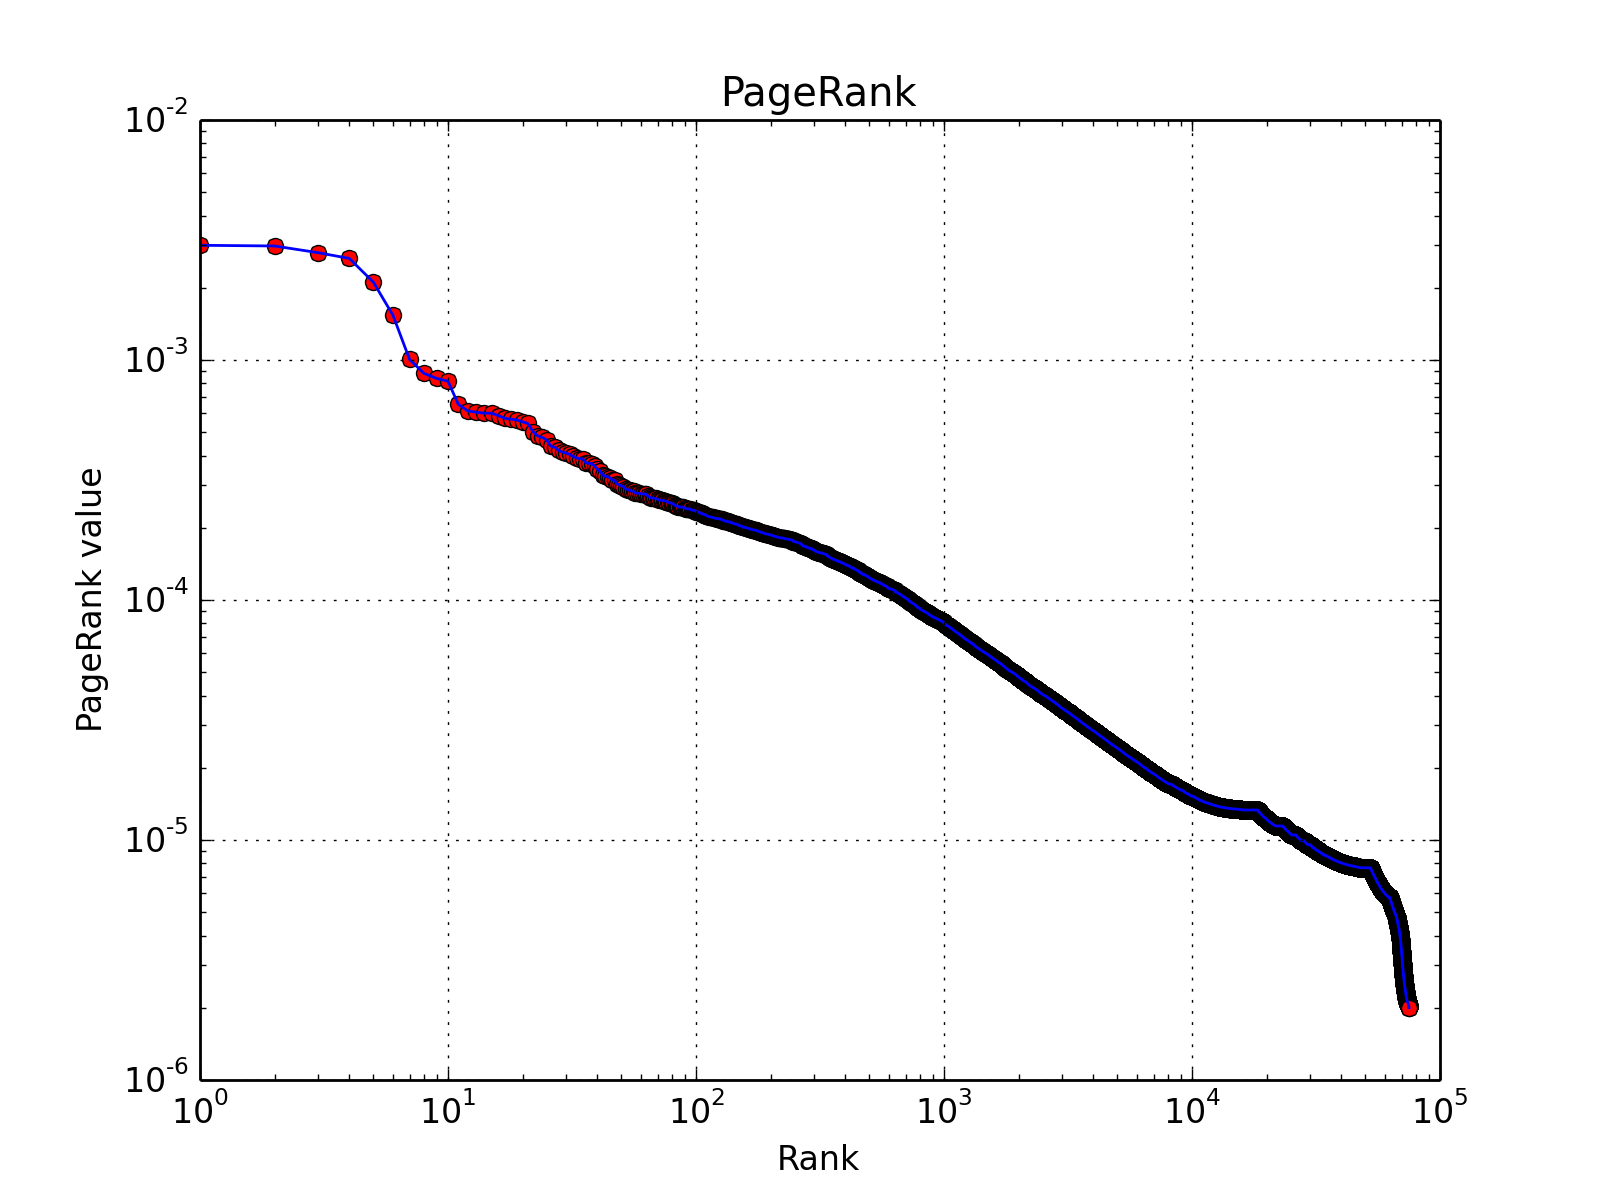
\includegraphics[width=0.35\textwidth]{FIG/pageRankoutput_soc-Slashdot0811-75000.png} 
\end{tabular}
\caption{PageRank plots of 10 graphs}
\label{fig:results}
\end{center}
\end{figure}

\textbf{Observation:}
\par Rank and PageRank of most graphs obey the power law. In log-log space as shown above, we can draw a line to fit the scatter points.

\subsection{Weakly connected components}

\begin{figure}[H]
\begin{center}
\begin{tabular}{ccc}
     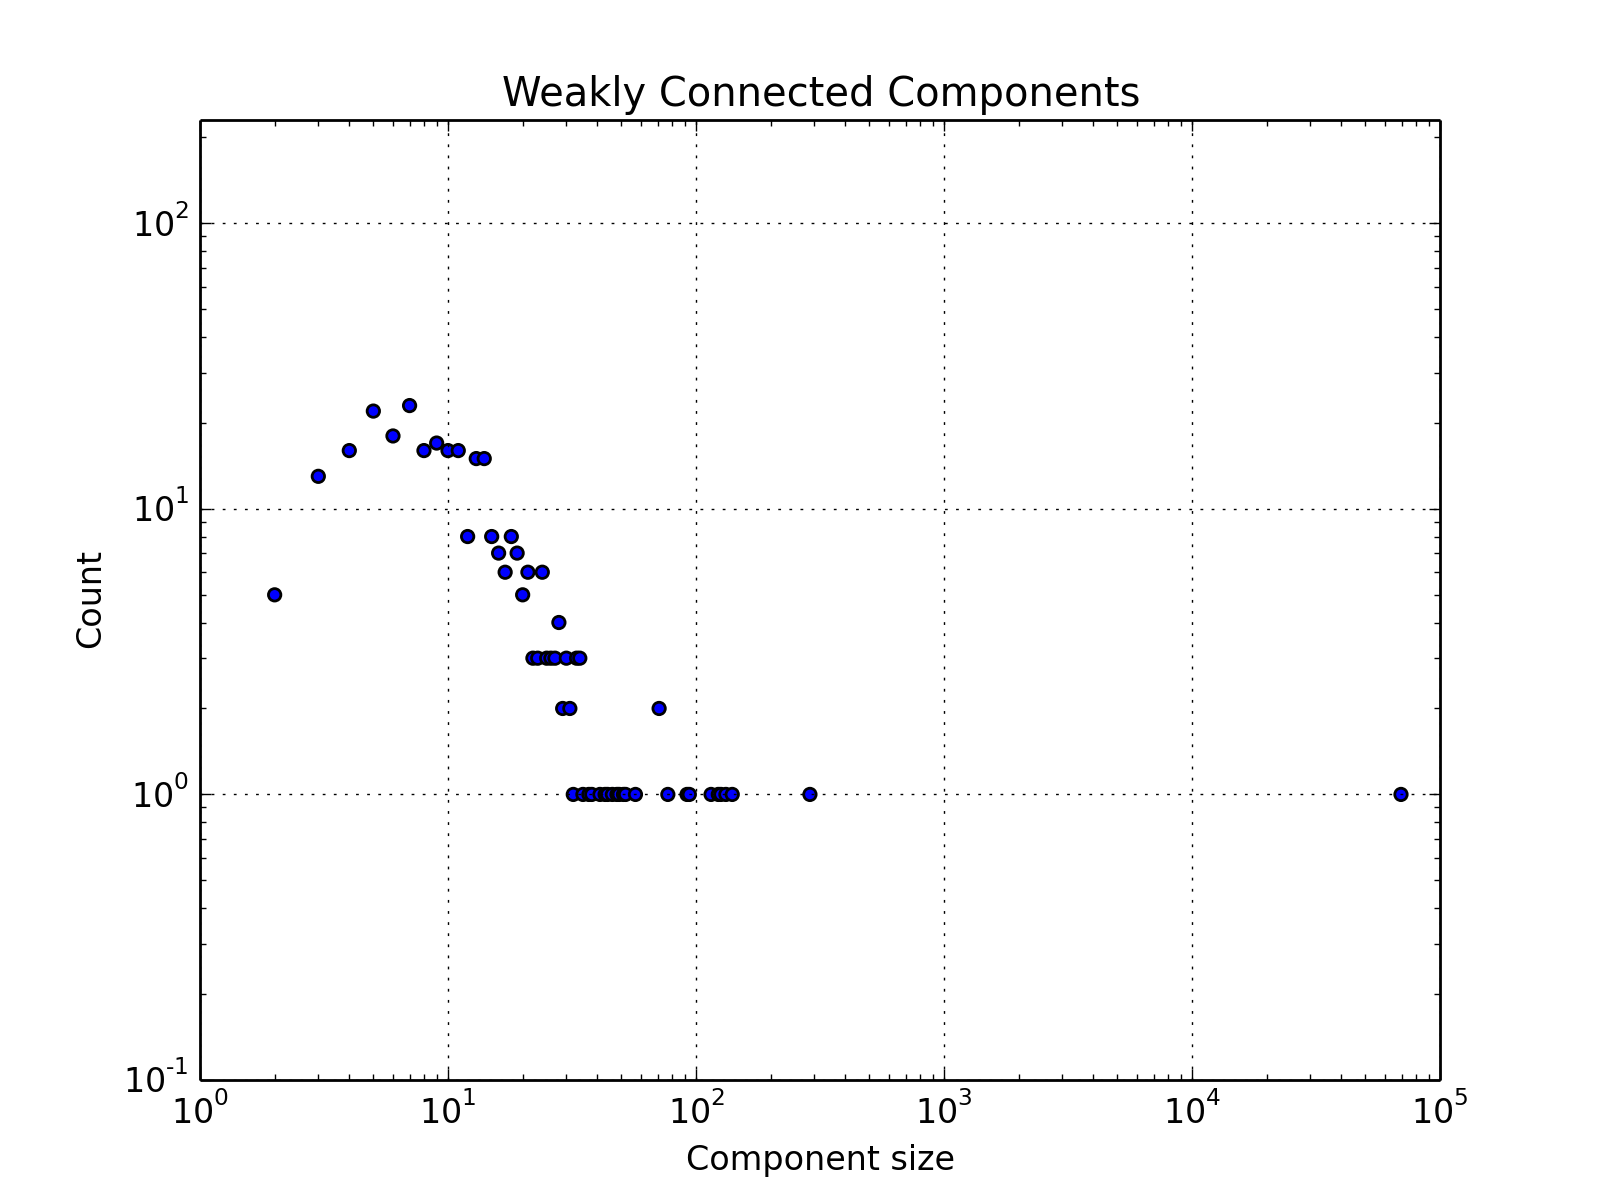
\includegraphics[width=0.35\textwidth]{FIG/plotConncompoutput_as-skitter.png} 
     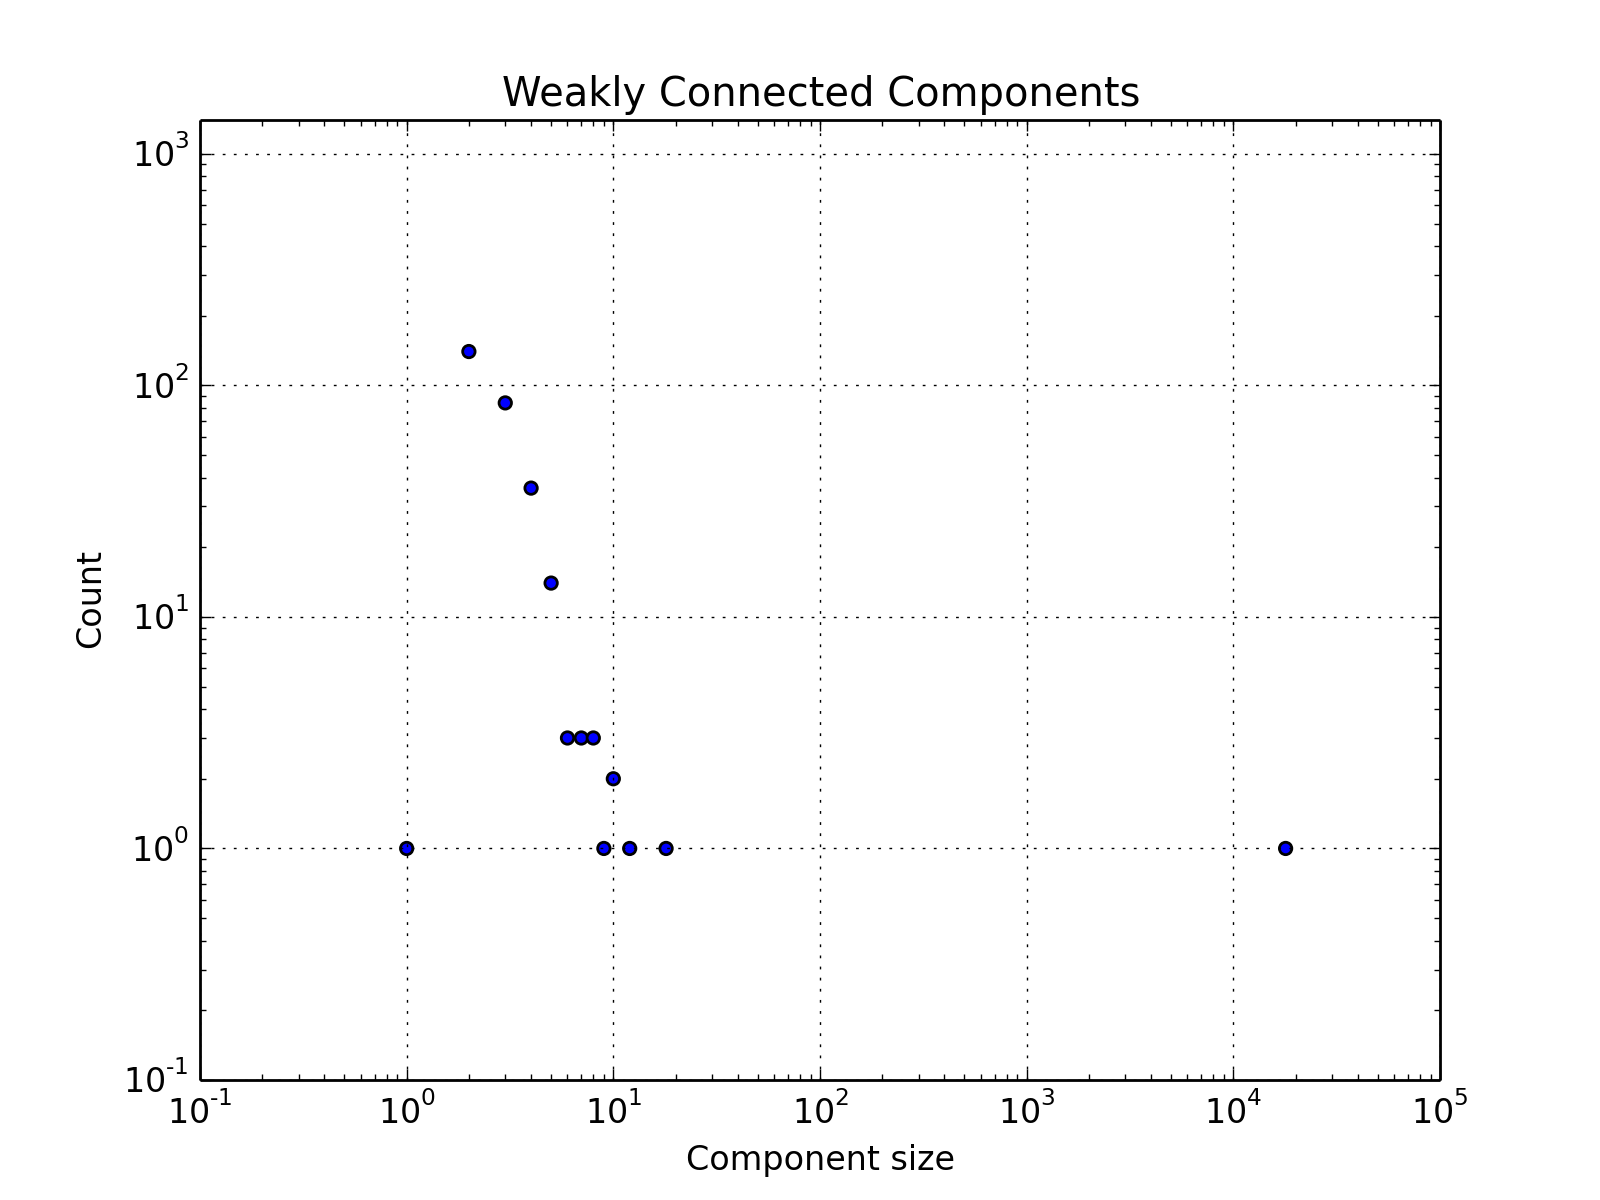
\includegraphics[width=0.35\textwidth]{FIG/plotConncompoutput_ca-AstroPh.png}
     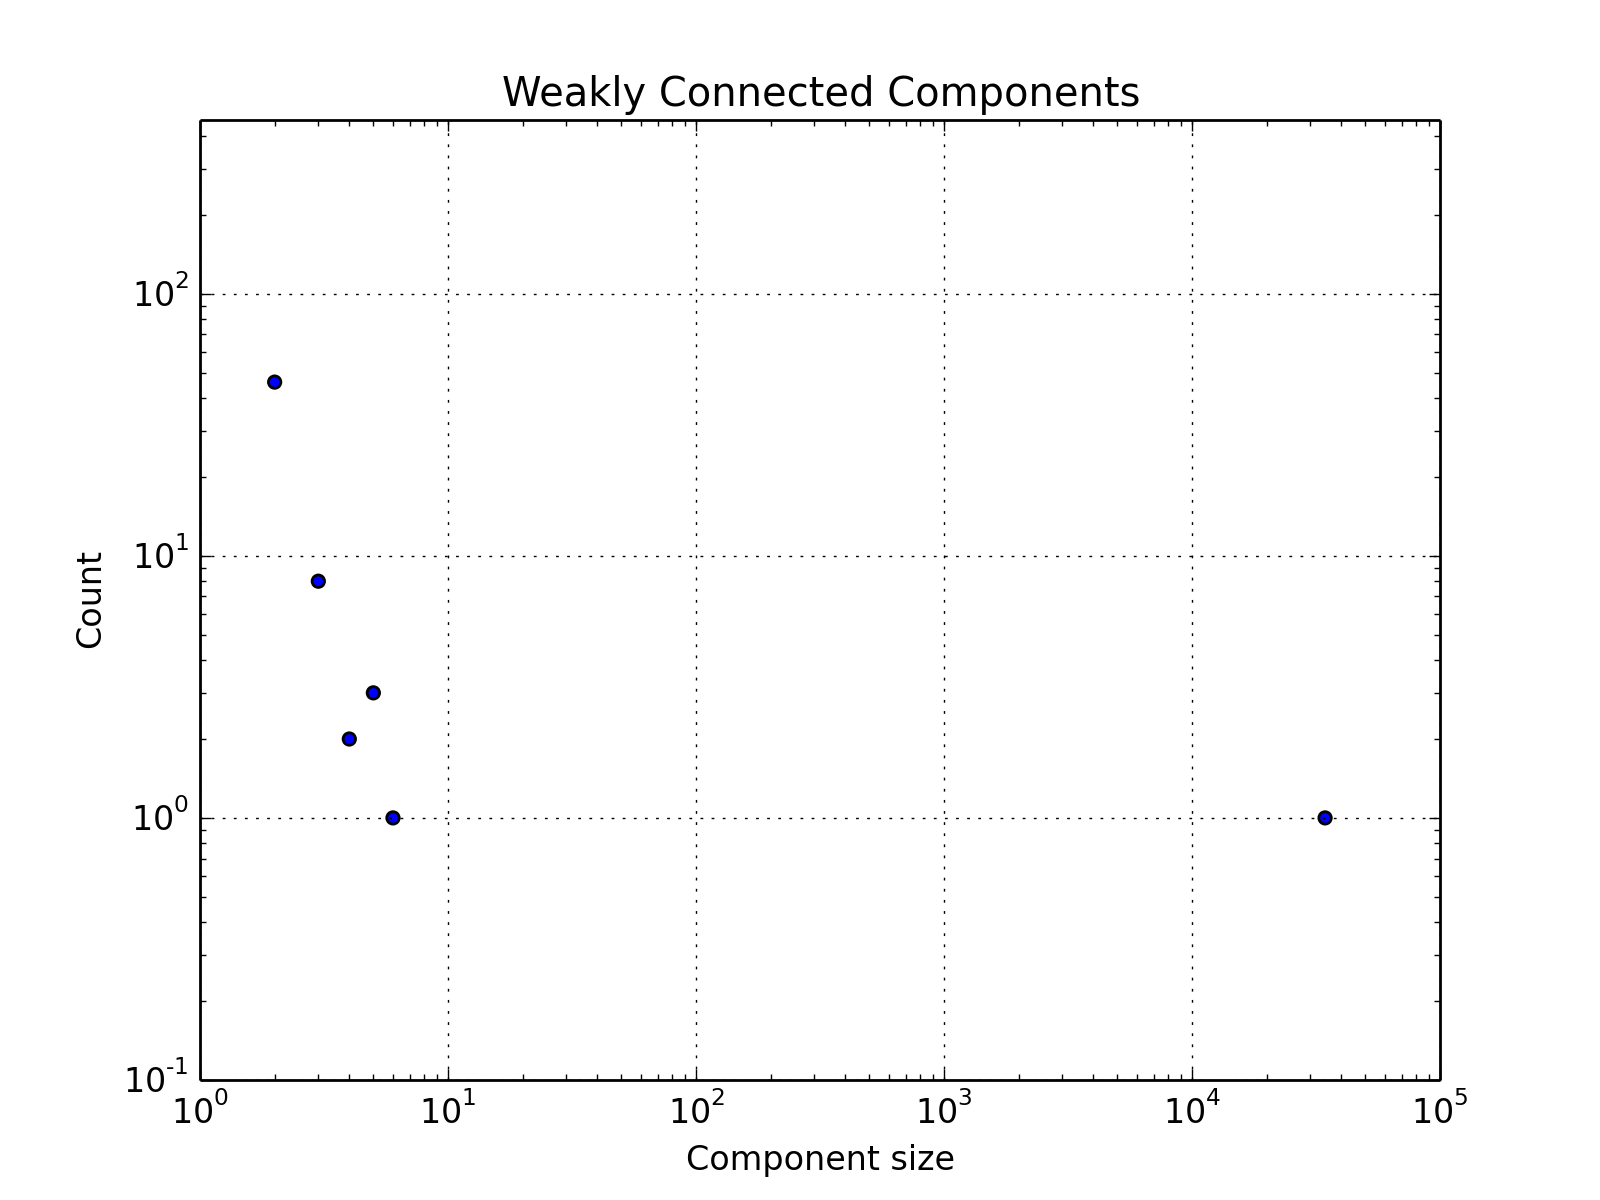
\includegraphics[width=0.35\textwidth]{FIG/plotConncompoutput_cit-HepPh.png} \\
     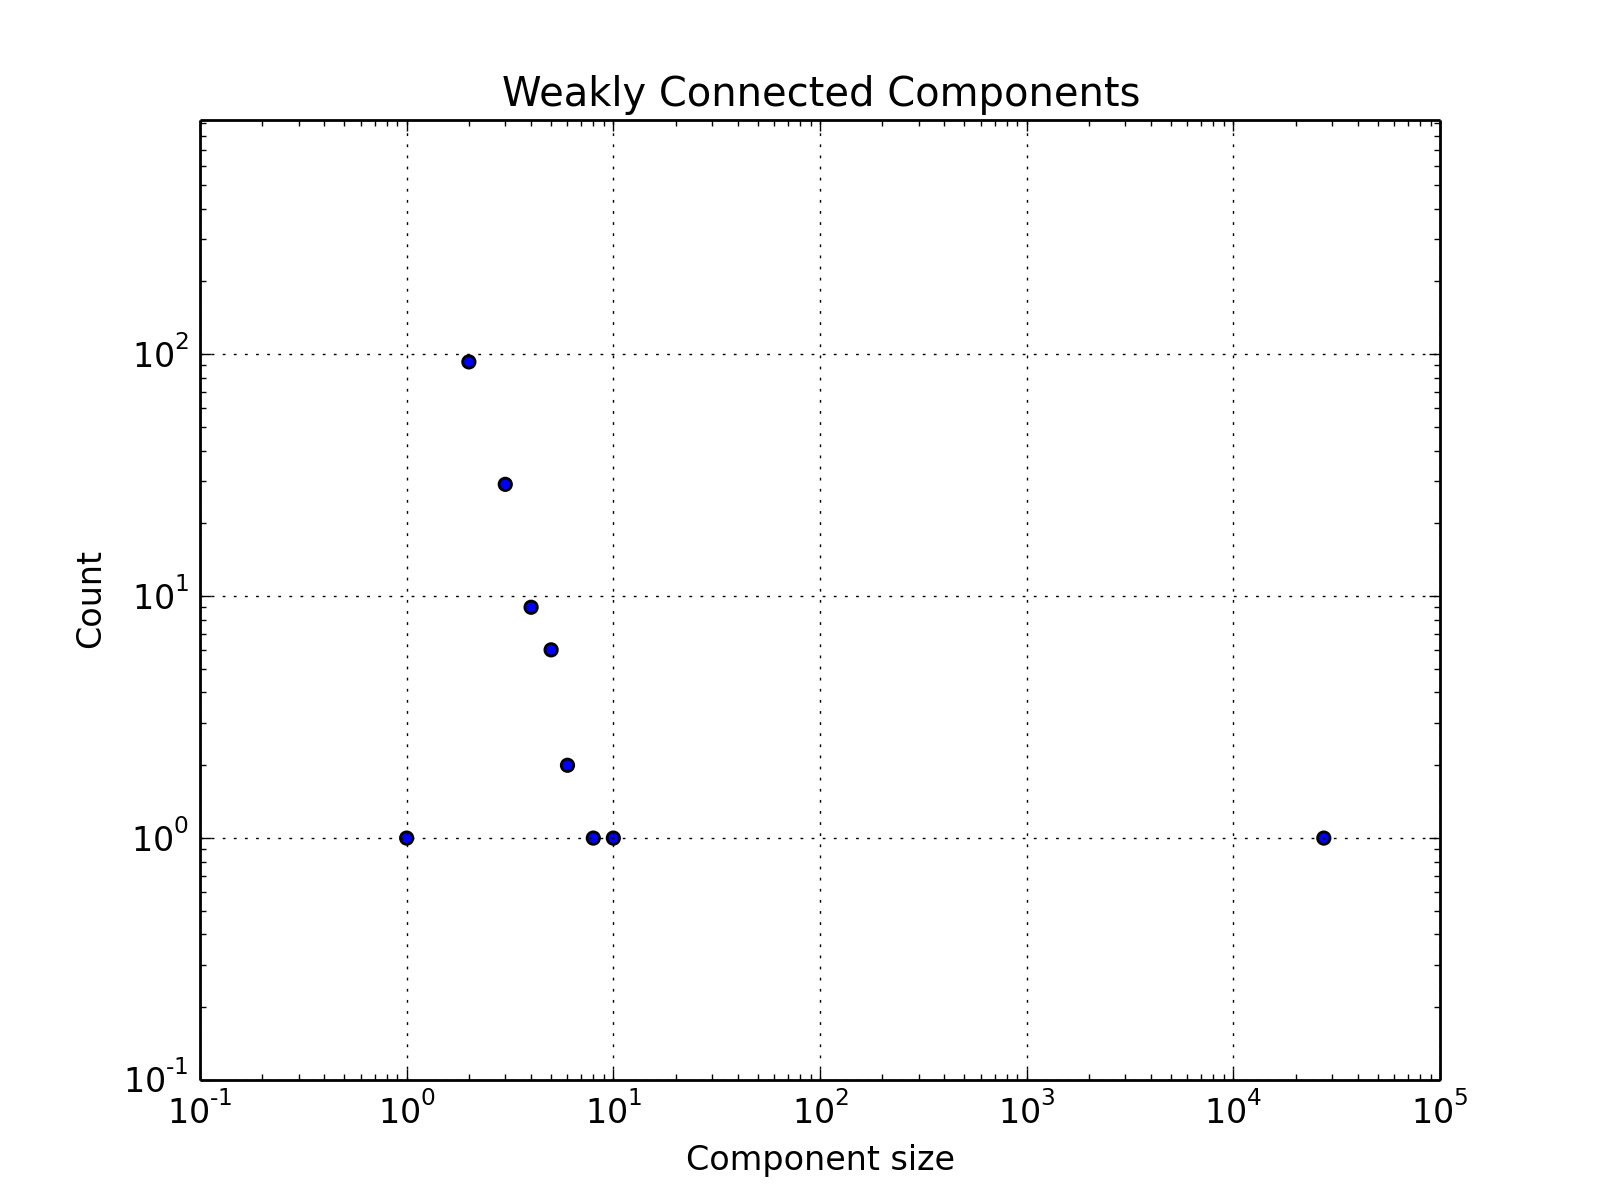
\includegraphics[width=0.35\textwidth]{FIG/plotConncompoutput_cit-HepTh.png} 
     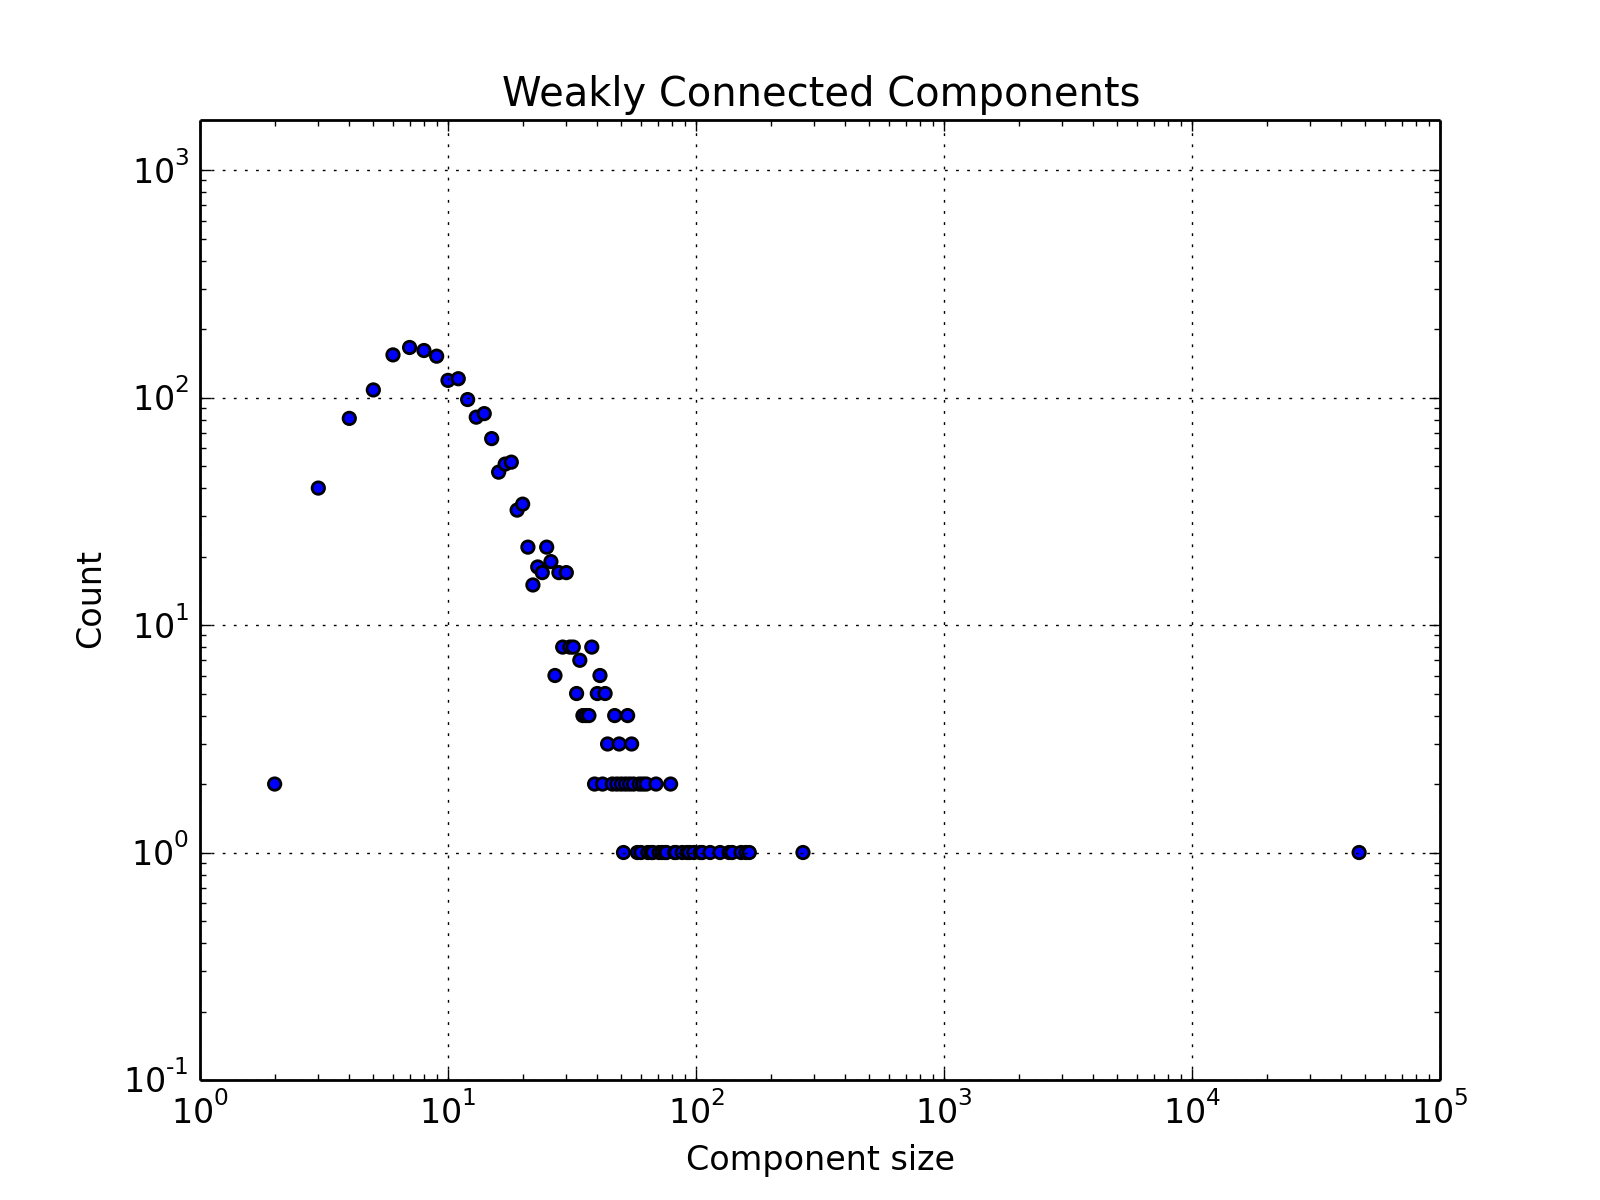
\includegraphics[width=0.35\textwidth]{FIG/plotConncompoutput_com-amazon.png} 
     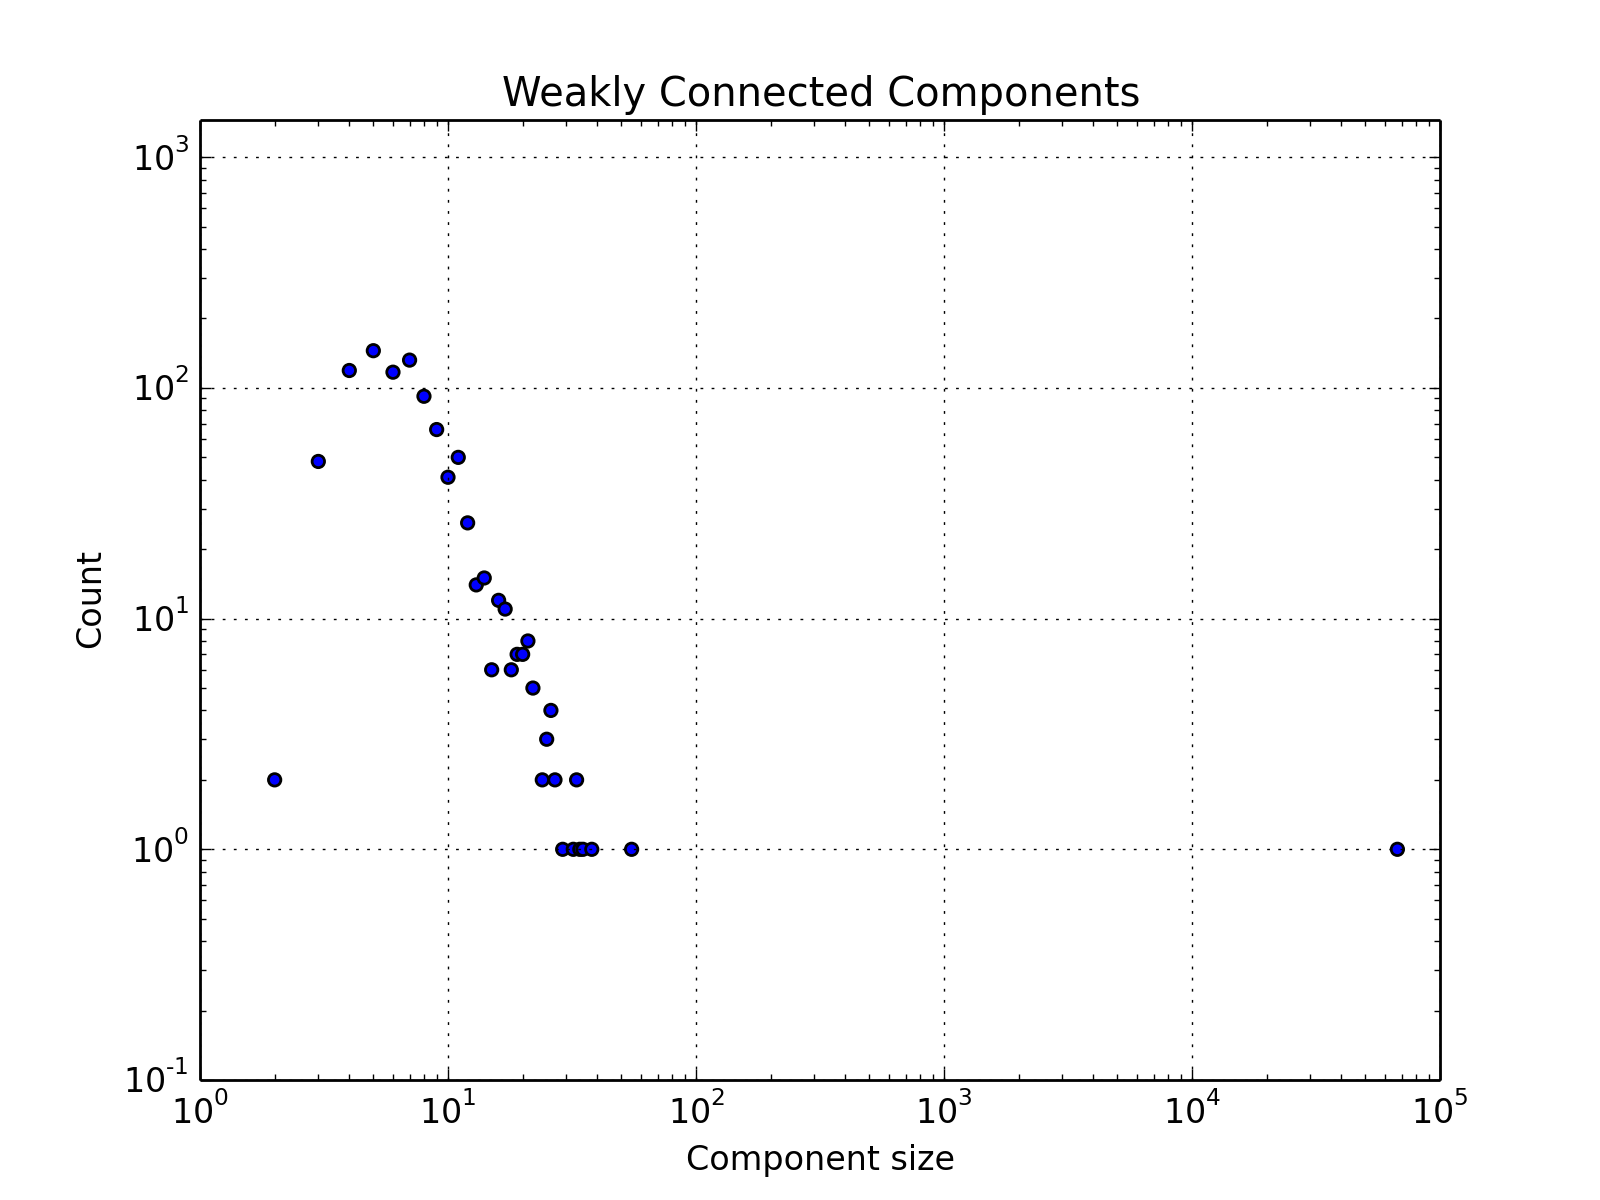
\includegraphics[width=0.35\textwidth]{FIG/plotConncompoutput_com-dblp.png} \\
     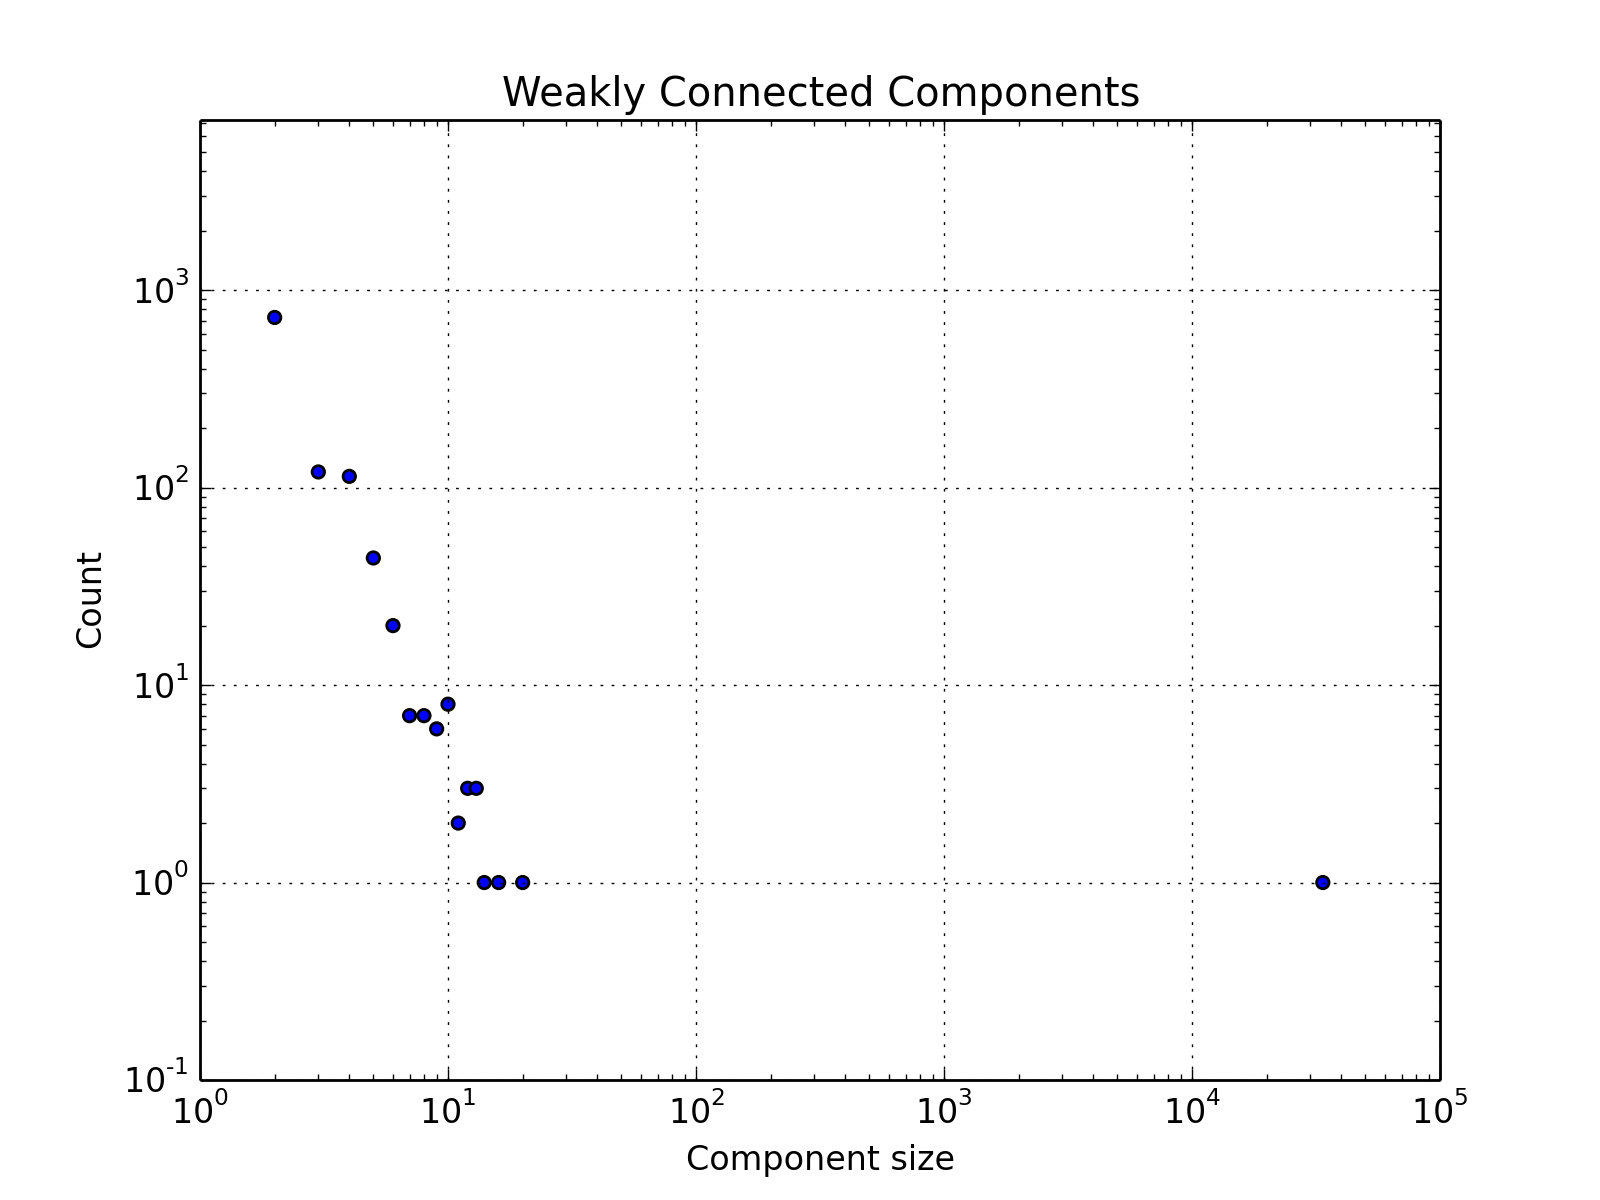
\includegraphics[width=0.35\textwidth]{FIG/plotConncompoutput_email-Enron.png} 
     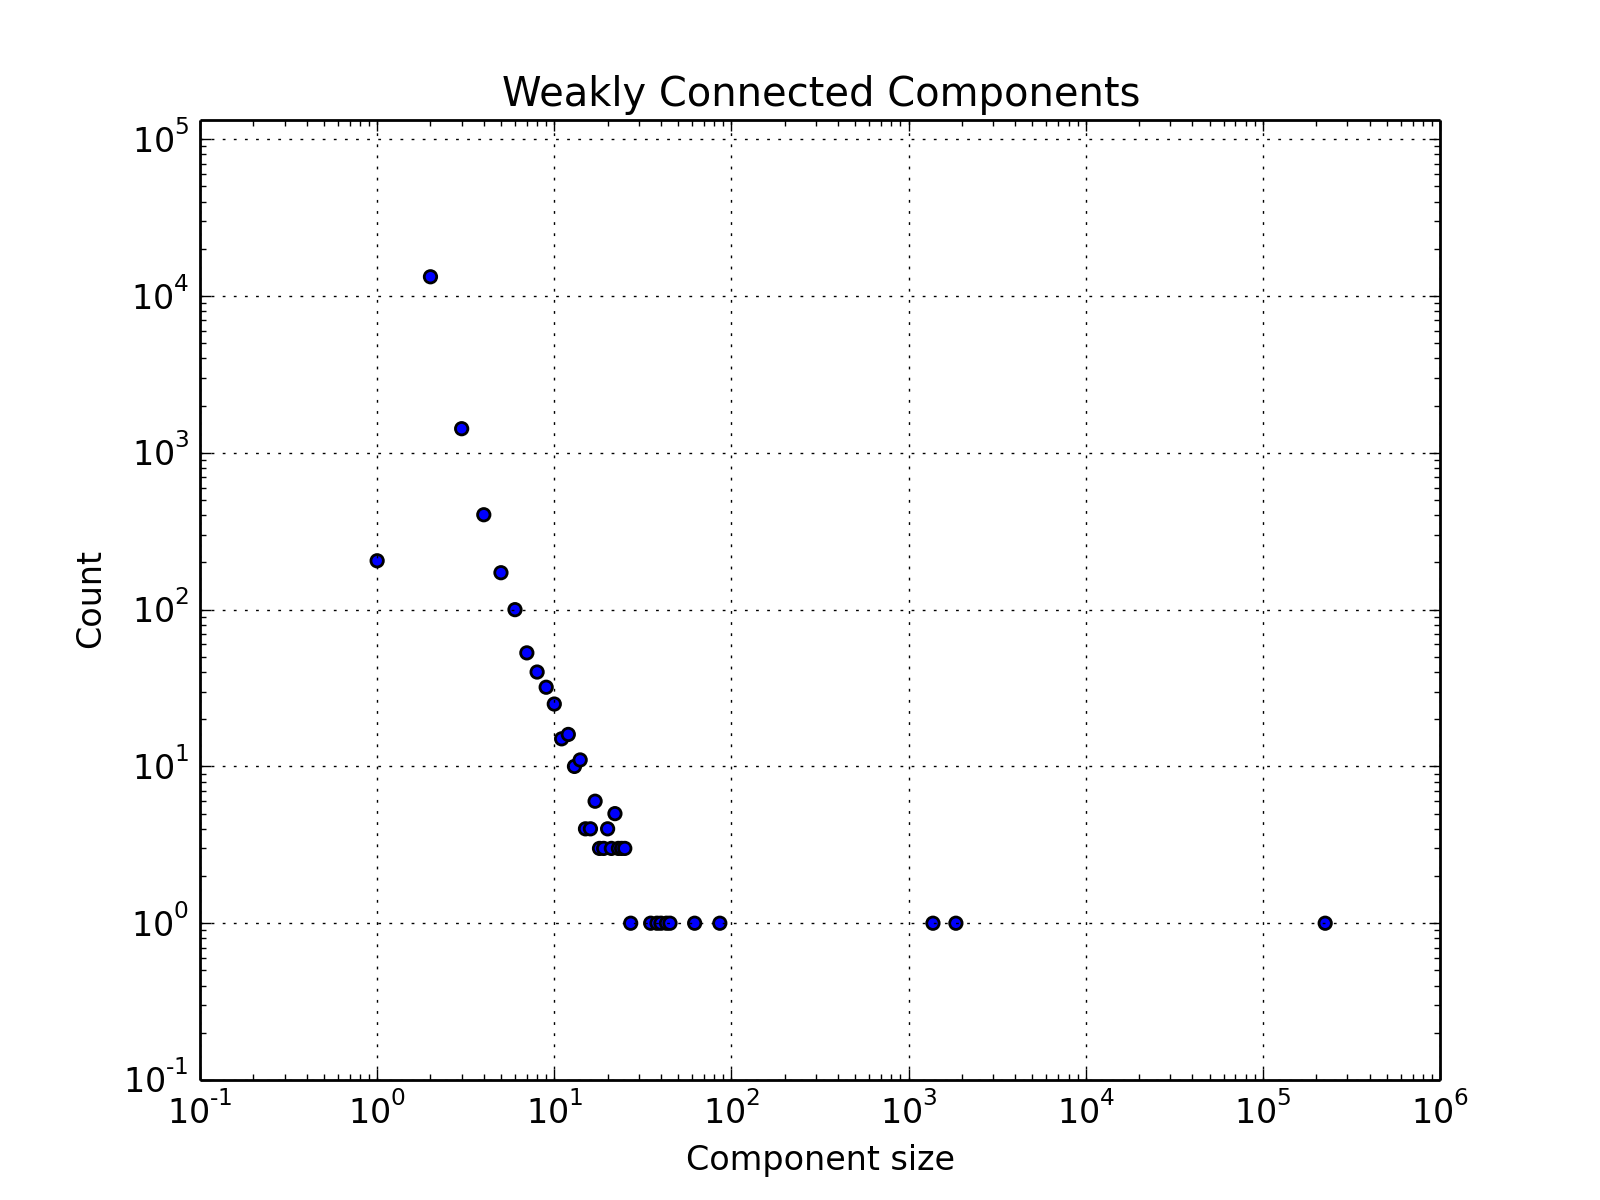
\includegraphics[width=0.35\textwidth]{FIG/plotConncompoutput_email-EuAll.png} 
     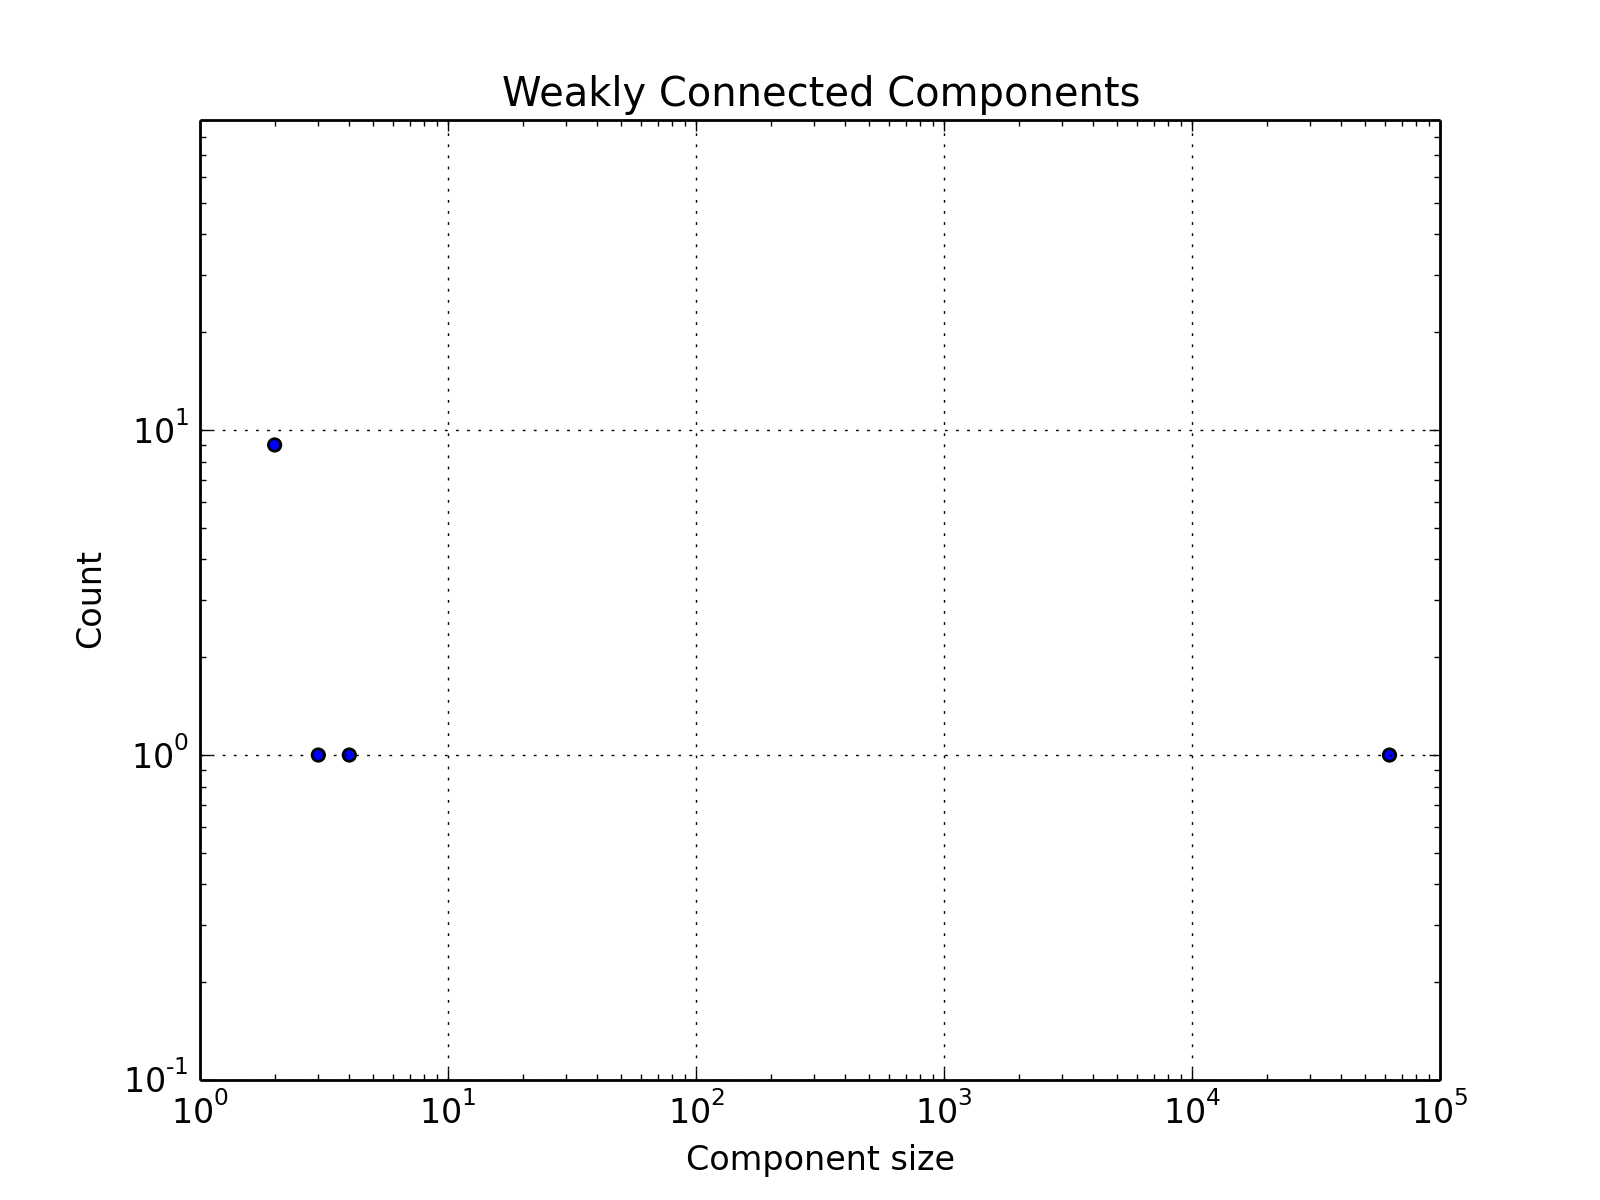
\includegraphics[width=0.35\textwidth]{FIG/plotConncompoutput_p2p-Gnutella31.png} \\
     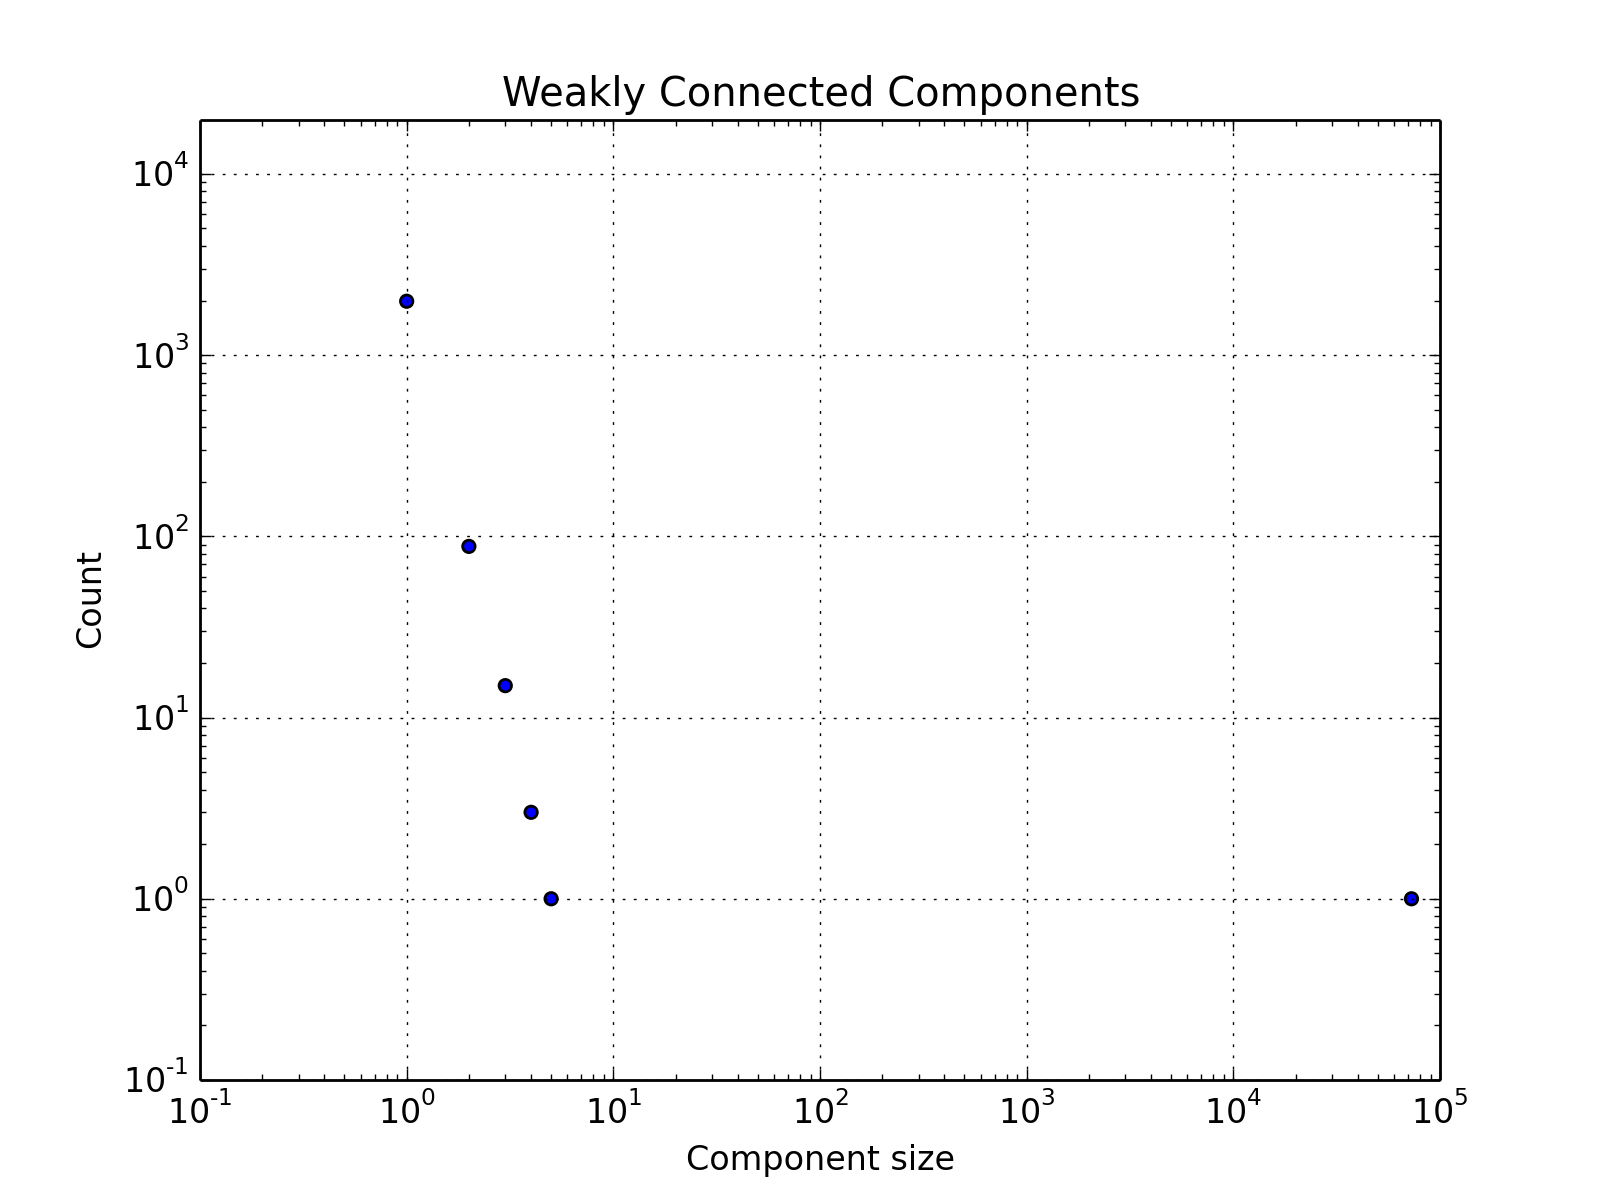
\includegraphics[width=0.35\textwidth]{FIG/plotConncompoutput_soc-Slashdot0811-75000.png} 
\end{tabular}
\caption{Weakly connected components plots of 10 graphs}
\label{fig:results}
\end{center}
\end{figure}

\textbf{Observation:}
\par Connected components of size 1 are essentially isolated points on the edge of the graph, the number of such components is generally small, as shown in the plots. Starting from size 2, the component size and corresponding count generally obeys the power law.

\subsection{Radius}

\begin{figure}[H]
\begin{center}
\begin{tabular}{ccc}
     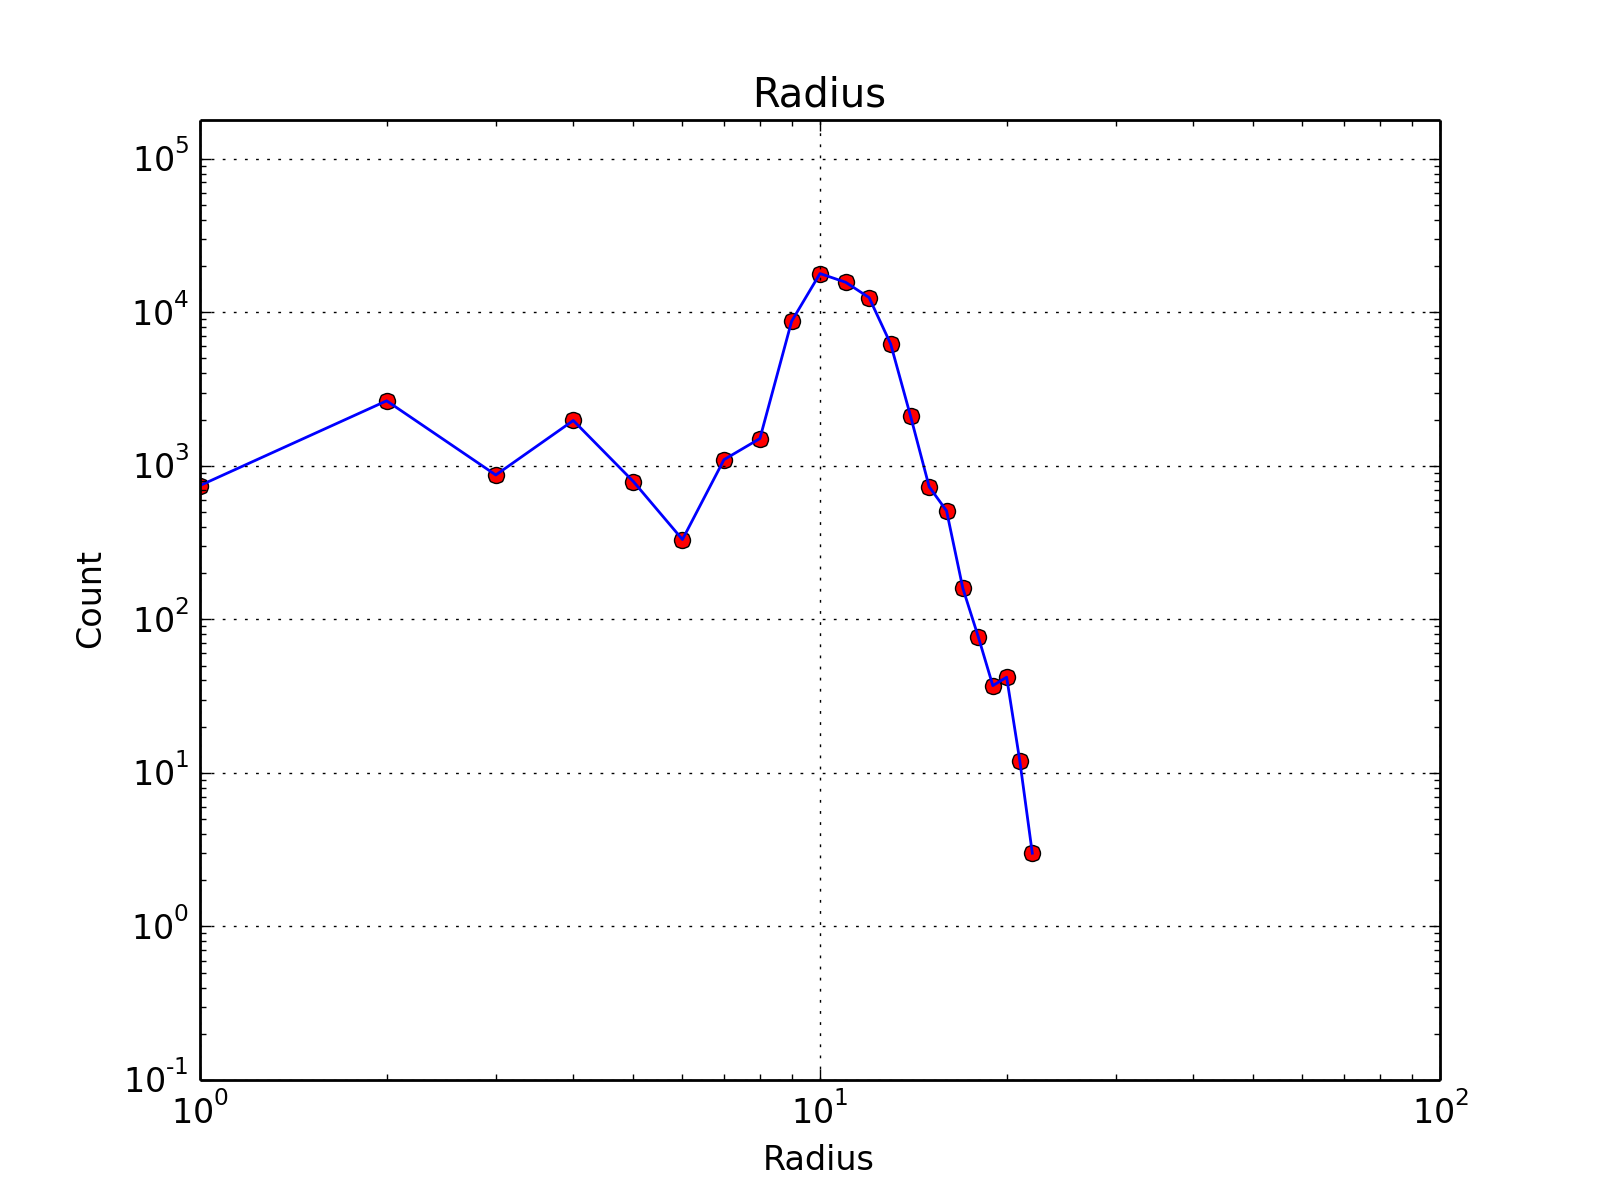
\includegraphics[width=0.35\textwidth]{FIG/Radiusoutput_as-skitter.png} 
     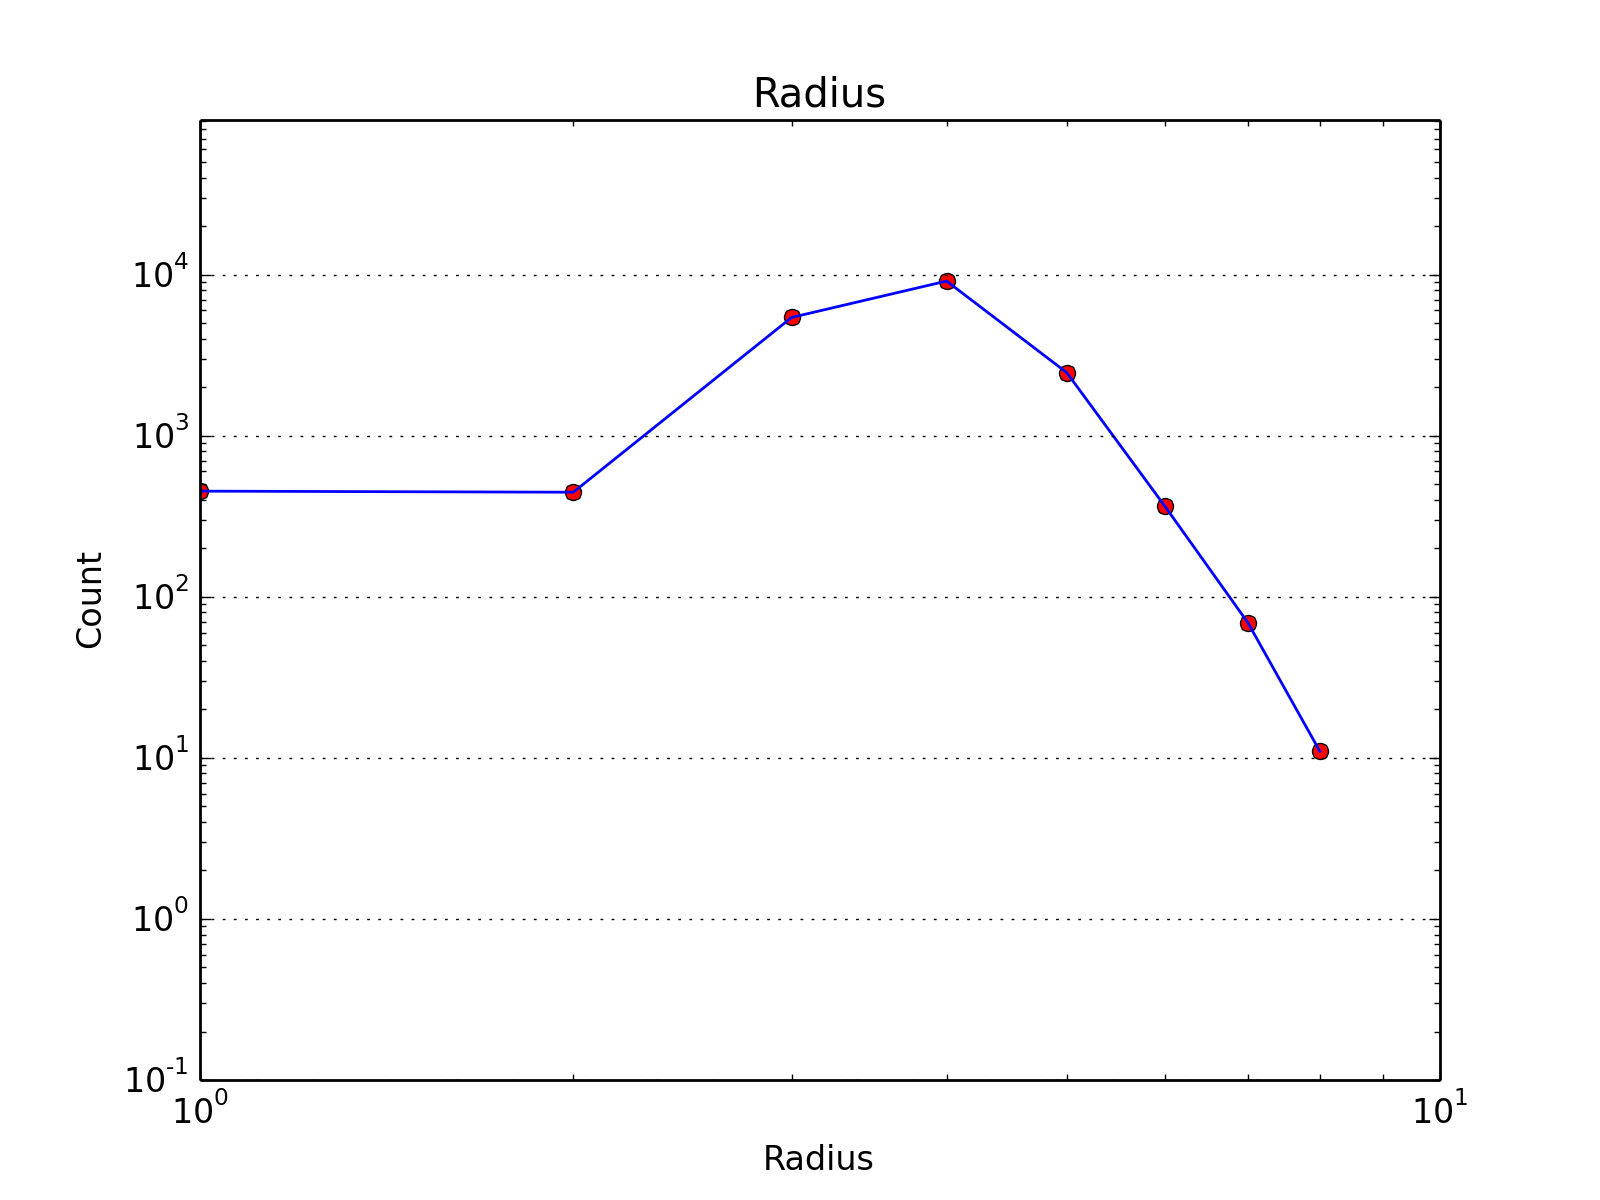
\includegraphics[width=0.35\textwidth]{FIG/Radiusoutput_ca-AstroPh.png}
     \includegraphics[width=0.35\textwidth]{FIG/Radiusoutput_cit-HepPh.png} \\
     \includegraphics[width=0.35\textwidth]{FIG/Radiusoutput_cit-HepTh.png} 
     \includegraphics[width=0.35\textwidth]{FIG/Radiusoutput_com-amazon.png} 
     \includegraphics[width=0.35\textwidth]{FIG/Radiusoutput_com-dblp.png} \\
     \includegraphics[width=0.35\textwidth]{FIG/Radiusoutput_email-Enron.png} 
     \includegraphics[width=0.35\textwidth]{FIG/Radiusoutput_email-EuAll.png} 
     \includegraphics[width=0.35\textwidth]{FIG/Radiusoutput_p2p-Gnutella31.png} \\
     \includegraphics[width=0.35\textwidth]{FIG/Radiusoutput_soc-Slashdot0811-75000.png} 
\end{tabular}
\caption{Radius plots of 10 graphs}
\label{fig:results}
\end{center}
\end{figure}

\textbf{Observation:}
\par Most Radius vs. Count plot has one distinct peak.

\subsection{KCore}

\begin{figure}[H]
\begin{center}
\begin{tabular}{ccc}
     \includegraphics[width=0.35\textwidth]{FIG/plotKcoreoutput_as-skitter.png} 
     \includegraphics[width=0.35\textwidth]{FIG/plotKcoreoutput_ca-AstroPh.png}
     \includegraphics[width=0.35\textwidth]{FIG/plotKcoreoutput_cit-HepPh.png} \\
     \includegraphics[width=0.35\textwidth]{FIG/plotKcoreoutput_cit-HepTh.png} 
     \includegraphics[width=0.35\textwidth]{FIG/plotKcoreoutput_com-amazon.png} 
     \includegraphics[width=0.35\textwidth]{FIG/plotKcoreoutput_com-dblp.png} \\
     \includegraphics[width=0.35\textwidth]{FIG/plotKcoreoutput_email-Enron.png} 
     \includegraphics[width=0.35\textwidth]{FIG/plotKcoreoutput_email-EuAll.png} 
     \includegraphics[width=0.35\textwidth]{FIG/plotKcoreoutput_p2p-Gnutella31.png} \\
     \includegraphics[width=0.35\textwidth]{FIG/plotKcoreoutput_soc-Slashdot0811-75000.png} 
\end{tabular}
\caption{KCore plots of 10 graphs}
\label{fig:results}
\end{center}
\end{figure}

\textbf{Observation:}
\par Some graphs show power law on the component size vs. count, e.g, graph No.4 and No.5. 

\section{K-Core Documentation}
   \label{sec:kcoredoc}
   \title{AlgorithmTemplate}
\documentclass[10pt]{article}
\usepackage{fullpage}
\usepackage{times}
\usepackage{fancyhdr,graphicx,amsmath,amssymb}
\usepackage[ruled,vlined]{algorithm2e}
\include{pythonlisting}

\begin{document}

\begin{algorithm}[h]
\KwIn{table, integer}
The core size k
The node connection graph,``GM\_TABLE\_UNDIRECT", that consists of: src\_id , target\_id \\
\KwOut{table}
A k-core graph that consists of: node id \\
%\nl \bf Pass\;
{\bf procedure:} \\
Create at tmp table that store the node-id and indegree count\\
{\bf While} the size tmp table still changes: \\
	~~~ find the node that the indegree is less than k \\
	~~~ remove the nodes from the ``GM\_TABLE\_UNDIRECT" \\
	~~~ calculate the tmp table again \\
output unique src\_id  \\
compute the weak component again  
\caption{{\bf Compute K-core Algorithm} \label{Algorithm}}

\end{algorithm}

\end{document}

\section{Graph summary and anomaly detection}
   \label{sec:graphsummary}
   \subsection{Datasets}
\par We studied 20 datasets, including 8 undirected graphs and 12 directed graphs. The details of the graphs are shown below.

\begin{table}[h]
\fontsize{8}{10}\selectfont
\begin{tabular}{lllll}
Dataset        & File                         & Category      & Directed & Description                            \\ \hline
Skitter        & as-skitter.ungraph-75000.txt & Physical      & N        & autonomous systems on web              \\
Caida          & as-Caida.undir.txt           & Physical      & N        & autonomous systems on web              \\
Enron          & email-Enron.ungraph.txt      & Communication & N        & email records between employees        \\
EU institution & email-EuAll.txt              & Communication & Y        & email records between employees        \\
Amazon         & com-amazon.ungraph-75000.txt & Co-occurence  & N        & bought X also bought Y                 \\
DBLP           & com-dblp.ungraph-75000.txt   & Coauthorship  & N        & coauthorship relationship              \\
Astro-Ph       & ca-AstroPh.txt               & Coauthorship  & Y        & coauthorship relationship              \\
Protein        & bio-protein-undir.txt        & Metabolic     & N        & metabolic interaction between proteins \\
JDK            & soft-jdkdependency.txt       & Software      & Y        & dependency between Java classes        \\
Spanish book   & text-spanishbook.txt         & Lexical       & Y        & word following relationship            \\
Gnutella       & p2p-Gnutella31.txt           & Computer      & Y        & connection between hosts               \\
Hep-Ph         & cit-HepPh.txt                & Citation      & Y        & citation relationship                  \\
Hep-Th         & cit-HepTh.txt                & Citation      & Y        & citation relationship                  \\
Cora           & cit-Cora.txt                 & Citation      & Y        & citation relationship                  \\
Hamsterster    & soc-hamsterster.undir.txt    & Social        & N        & social network friendship              \\
Youtube        & soc-Youtube-75000.undir.txt  & Social        & N        & social network friendship              \\
Slashdot       & soc-Slashdot0811-75000.txt   & Social        & Y        & directed friend/foe relationship       \\
Digg           & soc-digg.txt                 & Social        & Y        & reply from one user to another         \\
Flickr         & soc-flickr-75000.txt         & Social        & Y        & directed friendship                    \\
Pokec          & soc-pokec-75000.txt          & Social        & Y        & directed friendship                                       \\ \hline
\end{tabular}
\end{table}

In the following sections, we present our analysis on common features and distinctive patterns among these 20 dataset for various graph algorithms. Specifically, these algorithms include degree distributions, PageRank, weakly connected components, K-Core connected components with k=5, eigendecomposition and triangle count approximated from eigenvalues.

\subsection{Degree distributions}
\begin{figure}[H]
\begin{center}
\includegraphics[width=\textwidth]{FIG/degreedist.png}
\caption{Degree distribution of 20 graphs}
\end{center}
\end{figure}

\par Degree distributions of most of the graphs follow the power law(see Figure 4 above). However, for some of the graphs, counts of the smallest 10 degrees exhibit different patterns from power law. These graphs are discussed below.

\begin{itemize}
\item \textbf{Hep-Ph} The degree which has most corresponding nodes is 4 instead of 1, implying that most publications in this section have more than one citation relationship with others. Counts of nodes with degree more than 4 follow the power law.
\item \textbf{Astro-Ph} The degree which has most corresponding nodes is 4 instead of 1, implying that most publications in this section have more than one citation relationship with others. Counts of nodes with degree more than 4 follow the power law.
\item \textbf{Gnutella} There is a radical increasing of degree count at degree around 10, implying that there may be a popular application that requires about 10 hosts to connect to each other in order to work.
\item \textbf{Slashdot} The degree which has most corresponding nodes is 4 instead of 1, implying that most users have 4 friend/foe relationship with others, which means the friend/foe marking functionality is popular among users. Count of nodes with degree more than 4 follows the power law.
\item \textbf{JDK} The degree which has most corresponding nodes is 4 instead of 1, implying that most classes have 4 dependency relationship with others. Also, the counts for nodes with degree 50 to 90 does not show a obvious decreasing trend but rather stable, indicating that complex dependency relationship between JDK classes is common. Another discovery is that there is one node with much higher degree than others.
\item \textbf{Spanish book} The degree which has most corresponding nodes is 3 instead of 1, implying that most words have 3 adjacency relationship with other words(including itself).
\end{itemize}

\par Also, we spot that Caida, Protein, Youtube, Hamsterster datasets all have nodes with zero degree, which is possibly because these datasets are produced by random walk sampling of original datasets, making some nodes isolated.

\begin{figure}[H]
\begin{center}
\includegraphics[width=\textwidth]{FIG/indegreedist.png}
\caption{Indegree distribution of 12 directed graphs}
\end{center}
\end{figure}

\par Indegree distributions of most of the directed graphs follow the power law(see Figure 5 above). But for 2 of the 12 directed graphs, not the whole indegree distribution obeys the power law. These graphs are discussed below.

\begin{itemize}
\item \textbf{Astro-Ph} The indegree which has most corresponding nodes is 2 instead of 1, indicating that most publications are cited by 2 publications.
\item \textbf{Slashdot} The indegree which has most corresponding nodes is 2 instead of 1, indicating that most users have received two friend/foe marking.
\end{itemize}

There are also some other interesting facts observed from the indegree distributions:
\begin{enumerate}
\item There are only two nodes with zero indegree in the \textbf{Slashdot} dataset, implying that almost all users have been marked as friend/foe by at least one user.
\item In \textbf{JDK} dataset, there is one node with much higher indegree than other nodes. This nodes most probably represents $java.lang.Object$ class. Also, most classes has zero indegree, indicating most classes are leaves in the class hierarchy, depended by no other classes.
\item In three citation graphs \textbf{Cora}, \textbf{Hep-Ph}, \textbf{Hep-Th}, most publications have zero indegree, indicating that most publications are not cited by others.
\end{enumerate}

\begin{figure}[H]
\begin{center}
\includegraphics[width=\textwidth]{FIG/outdegreedist.png}
\caption{Outdegree distribution of 12 directed graphs}
\end{center}
\end{figure}

\par Outdegree distributions of most of the directed graphs follow the power law(see Figure 6 above). But for 5 of the 12 directed graphs, not the whole outdegree distribution obeys the power law. These graphs are discussed below.

\begin{itemize}
\item \textbf{Astro-Ph} The outdegree which has most corresponding nodes is 2 instead of 1, indicating that most publications cite 2 publications.
\item \textbf{Slashdot} The outdegree which has most corresponding nodes is 2 instead of 1, indicating that most users have made two friend/foe marking, again showing the popularity of this functionality.
\item \textbf{JDK} The outdegree which has most corresponding nodes is 4 instead of 1, indicating that most classes depend on 4 other classes. Also, only the middle part of the distribution, namely counts of nodes with outdegree 10 to 20, obey the power law.
\item \textbf{Gnutella} We spot a radical increasing of count starting from degree 7 to 10, and a radical decreasing from degree 10 to 11. This most probably indicates that the most common collaboration pattern in Gnutella network is for one host to connect to 8 to 10 hosts. Counts of nodes with degree more than 10 follow the power law.
\item \textbf{Spanish book} The outdegree which has most corresponding nodes is 2, indicating that most words in this book precedes two words(possibly itself). From the power law observed in the indegree and outdegree distribution of word adjacency in this book, it is clear that most words are used with only a few words together and few words are used very frequently with other words. This conforms to the nature of many languages.
\end{itemize}

Other interesting discoveries include:
\begin{enumerate}
\item In two of the social network datasets, \textbf{Flickr} and \textbf{Pokec}, nodes with zero outdegree is overwhelming, indicating that a substantial portion of users didn't actively make friends with other users, which means inactive users are quite common in social networks. In contrast, we spot in \textbf{Flickr} that one user has made about 2000 friends, more than twice of the second most, indicating that there is one extremely heavy user. Actually, there is a similar user in \textbf{Pokec} as well, but not so heavy. From these observations, we see that the activeness distribution caused by the nature of social network is the underlying reason of power law observed in both indegree and outdegree distribution.
\item Among three citation graphs, \textbf{Cora}, \textbf{Hep-Ph} and \textbf{Hep-Th}, most nodes in\textbf{Cora} has an outdegree of 1, much more than the nodes with zero outdegree, whereas in other two datasets the number of nodes with outdegree of 1 is close to the number of nodes with zero degree. This indicates that the research in Cora section is relatively more focused on established topics, while there are relatively more new topics in other two sections.
\end{enumerate}

\subsection{PageRank}
\begin{figure}[H]
\begin{center}
\includegraphics[width=\textwidth]{FIG/pagerank.png}
\caption{PageRank distribution of 20 graphs}
\end{center}
\end{figure}



\subsection{Weakly connected components}
\begin{figure}[H]
\begin{center}
\includegraphics[width=\textwidth]{FIG/conncomp.png}
\caption{Weakly connected components distribution of 20 graphs}
\end{center}
\end{figure}

We plot the size of connected component and count of components with that size in Figure 8. From the figure we can see 5 datasets are fully connected. For the remaining datasets, all of them have a very large component relative to the sizes of the other components. Among these datasets, most of them exhibits a power relation in the count and component size for connected components with small sizes. But some graphs exhibit a different relationship, as discussed below.

\begin{itemize}
\item random walk
\item Eu Institution
\item Hep-Th
\end{itemize}

\subsection{K-Core connected components with k=5}
\begin{figure}[H]
\begin{center}
\includegraphics[width=\textwidth]{FIG/conncomp-kcore.png}
\caption{5-Core connected components distribution of 20 graphs}
\end{center}
\end{figure}

\subsection{Eigendecomposition}
\subsection{Triangle count}
\begin{figure}[H]
\begin{center}
\includegraphics[width=\textwidth]{FIG/triangle.png}
\caption{Count of triangle of 20 graphs, approximated from eigenvalues}
\end{center}
\end{figure}

\section{Conclusion}
   \label{sec:conclusion}
   \par In this project, we learned that SQL can be effectively used to implement various graph algorithm. By implementing K-Core algorithm based on the framework provided by Graphminer, we got hands-on experience with SQL programming and deeper understanding of several graph algorithms, including the concept and implementation of degree distribution, PageRank, weakly connected components, radius and eigenvector. By experimenting with various index settings, we got a quantitive understanding of the benefits of index in complex SQL-based algorithms. By analyzing the results and plots of these graph algorithms, we identified the prevalence of power law and learned to use domain-specific knowledge to explain distinct patterns in various graph attributes.

\bibliography{BIB/christosref,BIB/other}
\bibliographystyle{plain}

\newpage
\pagenumbering{roman}
\tableofcontents


\end{document}
